\documentclass[9pt]{article}
\usepackage[english]{babel}
\usepackage{amsmath,amsthm}
\usepackage{amsfonts}
\usepackage{graphicx}
\usepackage[margin=0.2in]{geometry}
\newcommand{\setlinespacing}[1]{\setlength{\baselineskip}{#1 \defbaselineskip}}
\newcommand{\doublespacing}{\setlength{\baselineskip}{2.0 \defbaselineskip}}
\newcommand{\singlespacing}{\setlength{\baselineskip}{\defbaselineskip}}
\newcommand{\A}{{\cal A}}
\newcommand{\h}{{\cal H}}
\newcommand{\s}{{\cal S}}
\newcommand{\W}{{\cal W}}
\newcommand{\BH}{\mathbf B(\cal H)}
\newcommand{\KH}{\cal  K(\cal H)}
\newcommand{\Real}{\mathbb R}
\newcommand{\Complex}{\mathbb C}
\newcommand{\Field}{\mathbb F}
\newcommand{\RPlus}{[0,\infty)}
\newcommand{\norm}[1]{\left\Vert#1\right\Vert}
\newcommand{\essnorm}[1]{\norm{#1}_{\text{\rm\normalshape ess}}}
\newcommand{\abs}[1]{\left\vert#1\right\vert}
\newcommand{\set}[1]{\left\{#1\right\}}
\newcommand{\seq}[1]{\left<#1\right>}
\newcommand{\eps}{\varepsilon}
\newcommand{\To}{\longrightarrow}
\newcommand{\RE}{\operatorname{Re}}
\newcommand{\IM}{\operatorname{Im}}
\newcommand{\Poly}{{\cal{P}}(E)}
\newcommand{\EssD}{{\cal{D}}}
\newcommand{\field}[1]{\mathbb{#1}}
\newcommand{\C}{\field{C}}
\newcommand{\R}{\field{R}}
\newcommand{\script}[1]{\mathcal{#1}}
\newcommand{\fall}{\; \forall \;}
\newcommand{\exts}{\; \exists \;}
\newcommand{\mbf}[1]{\mathbf{#1}}
\newcommand{\binomial}[2]{\biggl( \begin{array}{c}  #1 \\ #2  \\ \end{array} \biggr) }
\newcommand{\fderiv}[2]{ \frac{d}{ d #1} \: #2}
\newcommand{\sderiv}[2]{ \frac{d^2}{ d^2 #1} \: #2}
\newcommand{\pfderiv}[2]{ \frac{\partial}{ \partial #1} \: #2}
\newcommand{\psderiv}[2]{ \frac{\partial^2}{ \partial^2 #1} \: #2}
\newcommand{\mat}[1]{\mathbf{#1}}
\DeclareSymbolFont{AMSb}{U}{msb}{m}{n}
\DeclareMathSymbol{\dblz}{\mathalpha}{AMSb}{"5A}
\DeclareMathSymbol{\dblr}{\mathalpha}{AMSb}{"52}
\DeclareMathSymbol{\dblt}{\mathalpha}{AMSb}{"54}
\DeclareMathSymbol{\dblq}{\mathalpha}{AMSb}{"51}
\DeclareMathSymbol{\dbln}{\mathalpha}{AMSb}{"4E}
\DeclareMathSymbol{\dblf}{\mathalpha}{AMSb}{"46}
\DeclareMathSymbol{\dblc}{\mathalpha}{AMSb}{"43}
\DeclareMathSymbol{\dbld}{\mathalpha}{AMSb}{"44}
\theoremstyle{plain}
\newtheorem{thm}{Theorem}[section]
\newtheorem{cor}[thm]{Corollary}
\newtheorem{lem}[thm]{Lemma}
\newtheorem{prop}[thm]{Proposition}
\theoremstyle{definition}
\newtheorem{defn}{Definition}[section]
\theoremstyle{remark}
\newtheorem{rem}{Remark}[section]
\numberwithin{equation}{section}
\renewcommand{\theequation}{\thesection.\arabic{equation}}
\begin{document}
\title{Regression of KL Software Distribution   }
\author{KL Software Libraries}
\date{Sun May 11 18:11:14 2014
}
\maketitle
\textbf{ KL Library test output.  This LaTex file and the associated diagrams are produced by the KL software libraries.}
\subsubsection{Testing binary writer}
Binary writer Speedup 1GB Double Matrix 1.77916
Binary reader Speedup 1GB Double Matrix 441.717
Binary writer Speedup 1GB Double vector 0.368195
Binary reader Speedup 1GB Double Matrix 586.932
QueryPerformanceCounter  =  28.9483
\subsubsection{Fast Gauss Transform}
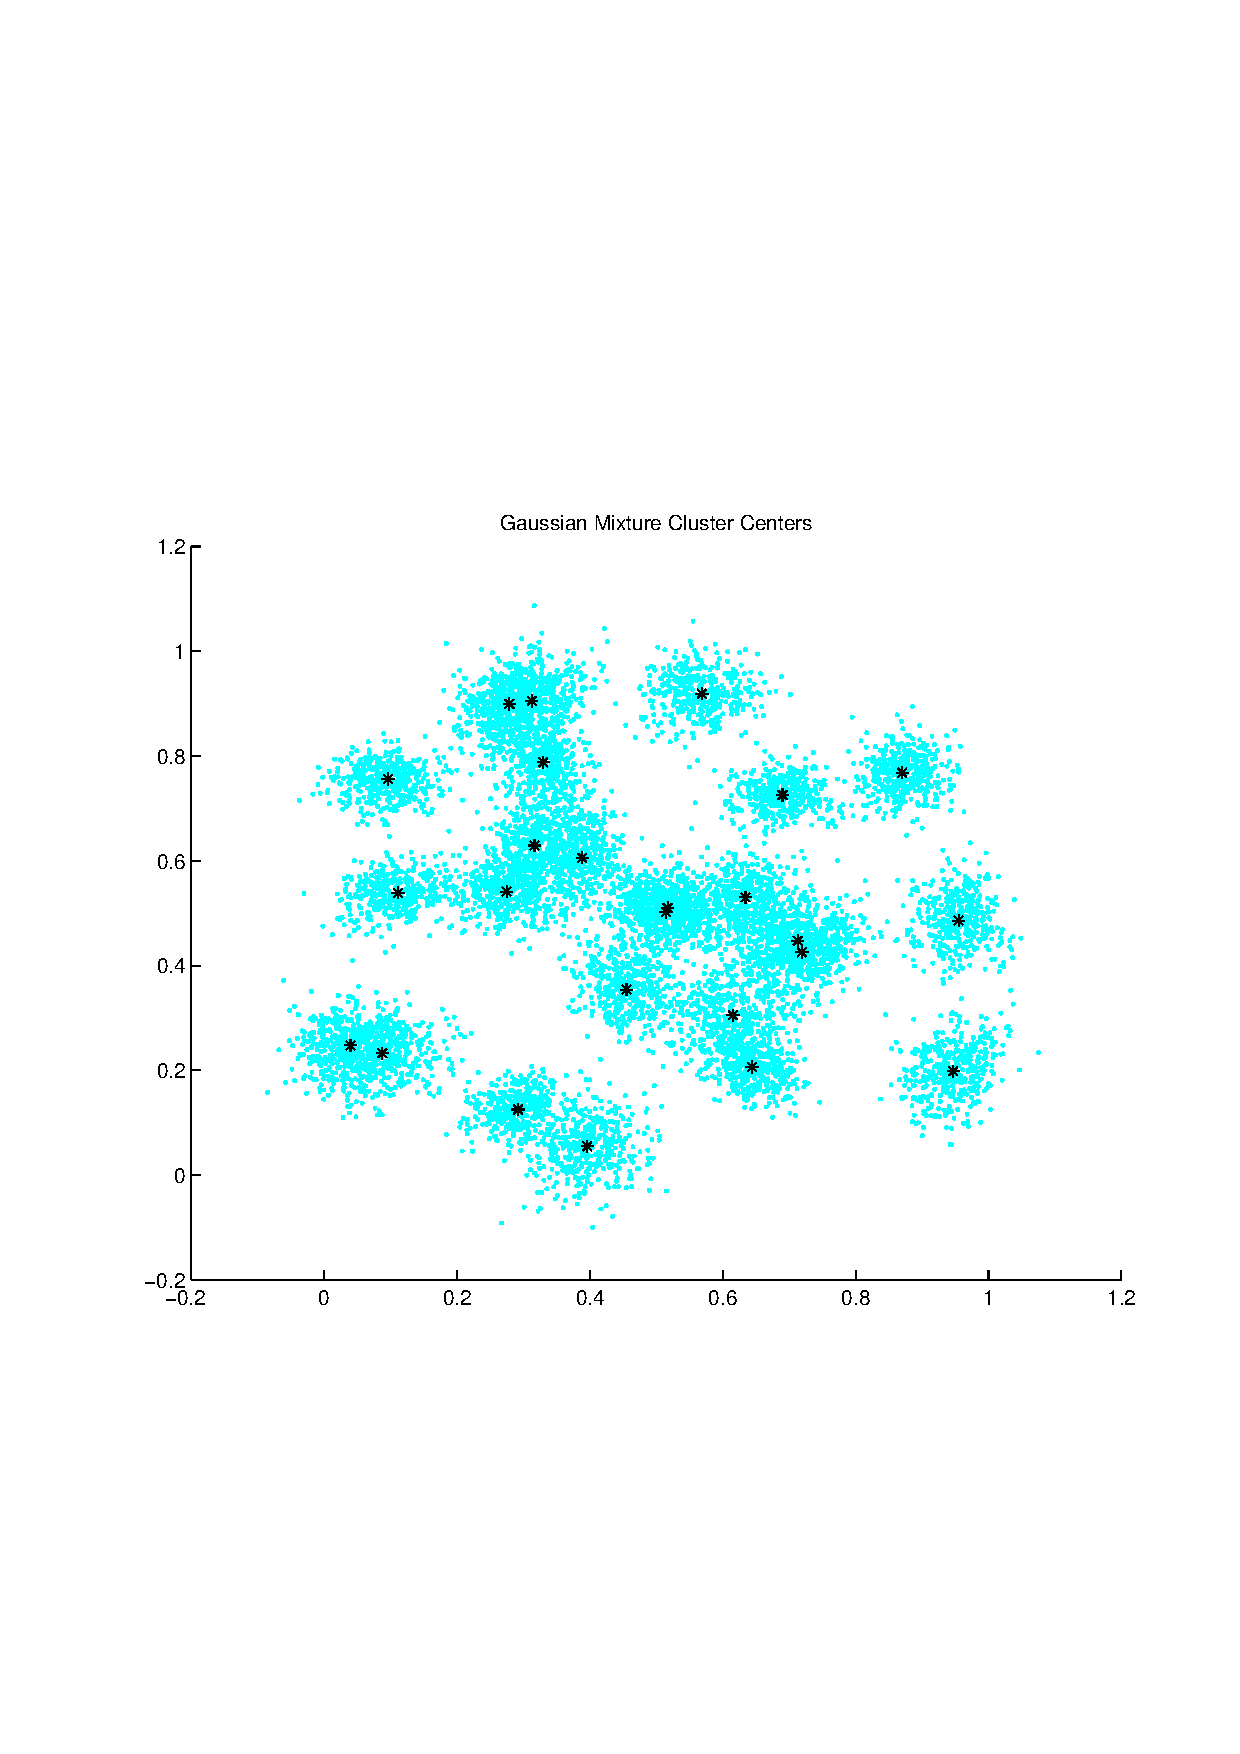
\includegraphics[width=10.0cm,height=10.0cm]{GaussianMixture_ClusterCenters25_Centers.pdf}

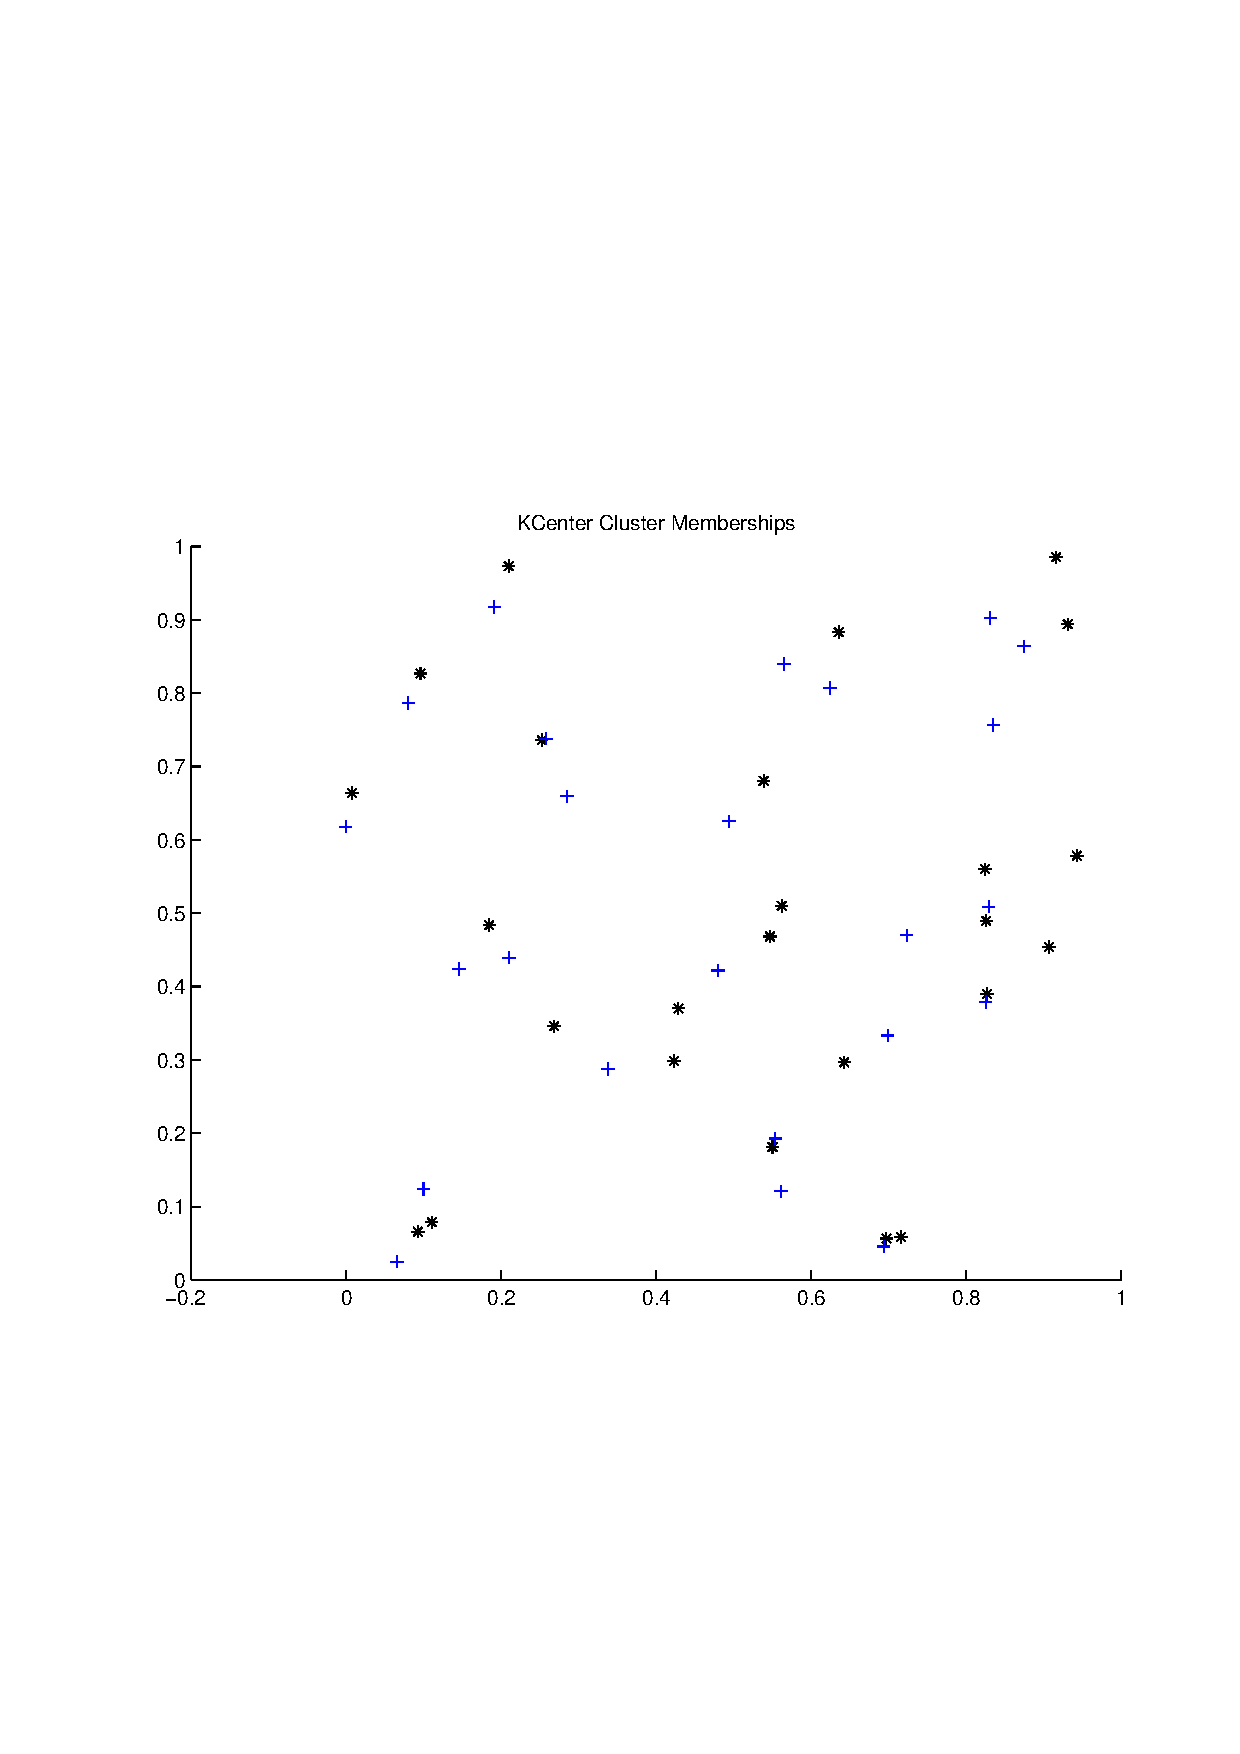
\includegraphics[width=10.0cm,height=10.0cm]{KCenterClusterMemberships_25_Centers.pdf}

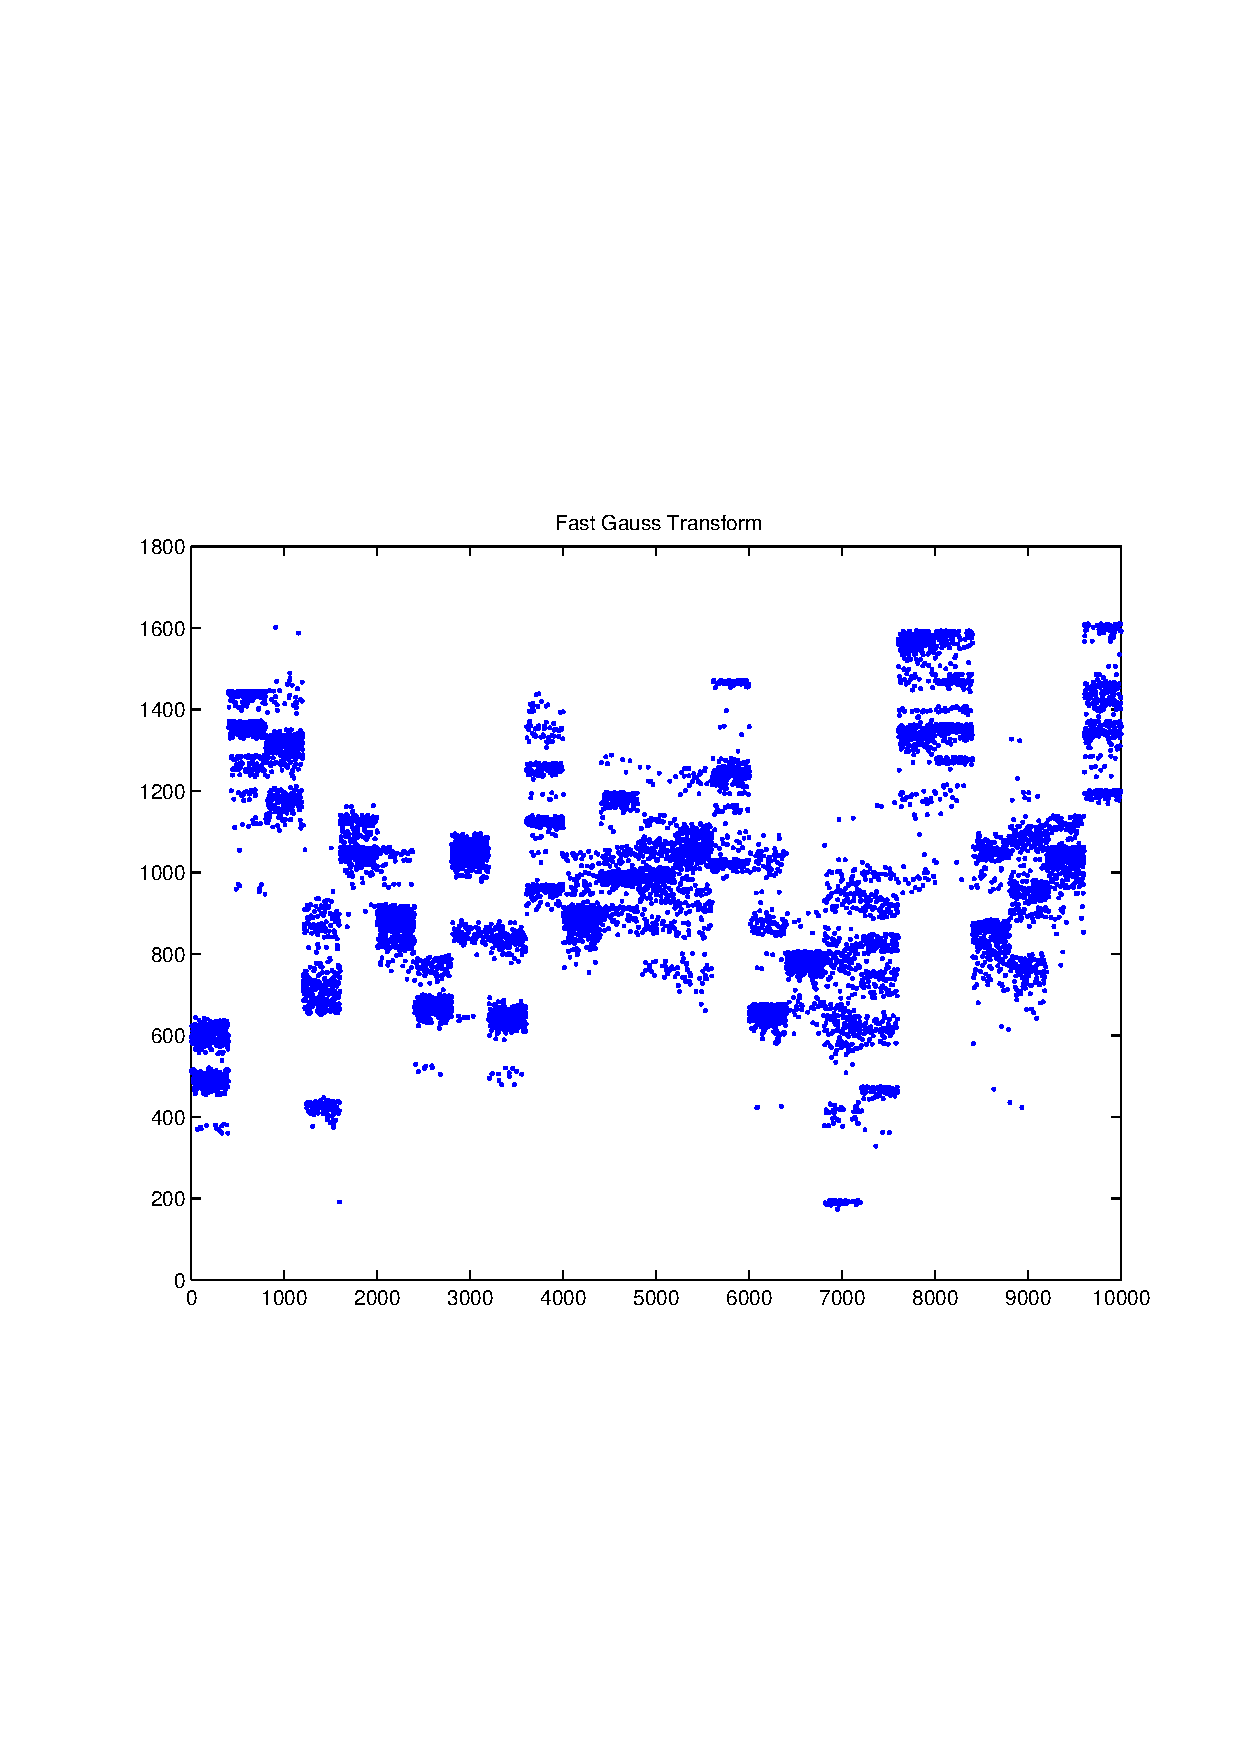
\includegraphics[width=10.0cm,height=10.0cm]{FGT25_Centers.pdf}

QueryPerformanceCounter  =  14.0082
\subsubsection{Testing Gaussian Mixture Point Cloud and Latex Plotting Capabilities.}
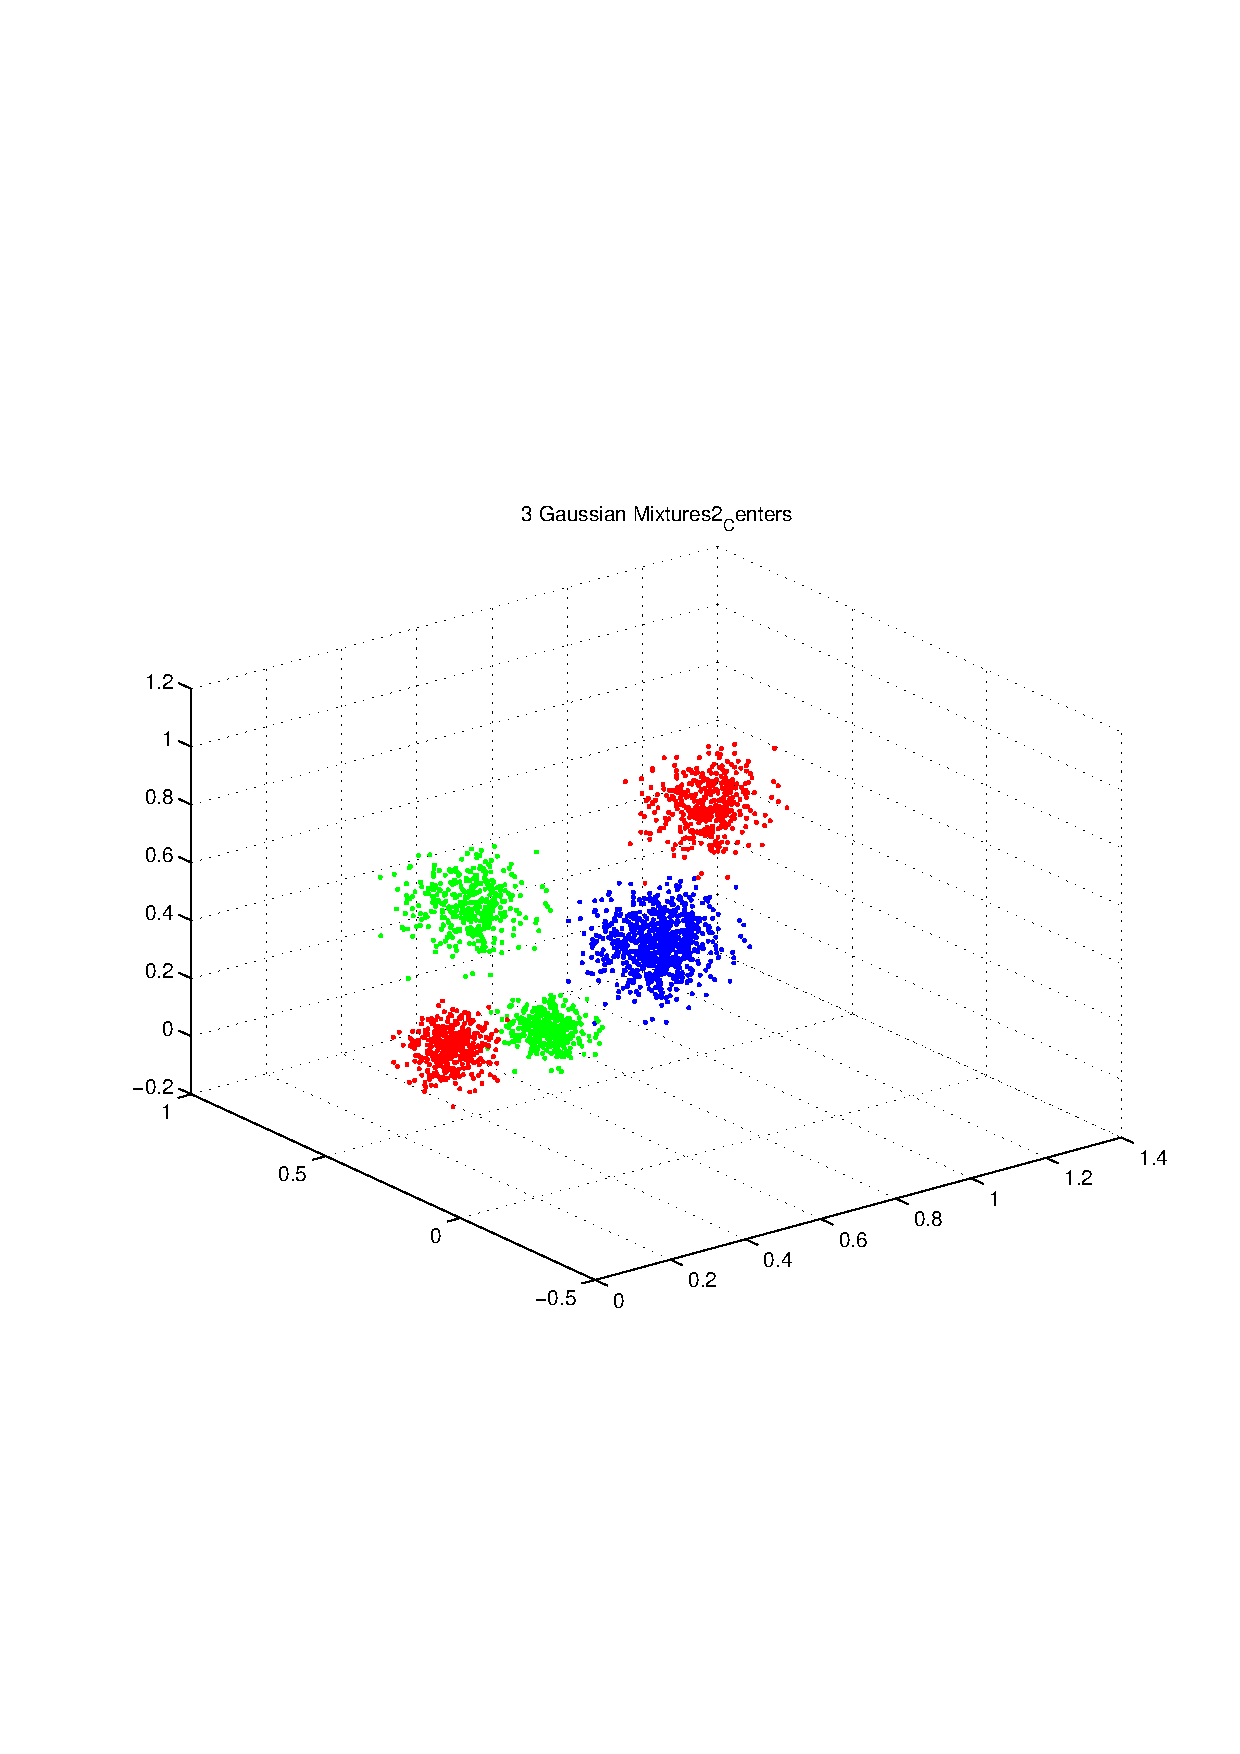
\includegraphics[width=10.0cm,height=10.0cm]{GaussianMixture_Dim_3_Centers2.pdf}

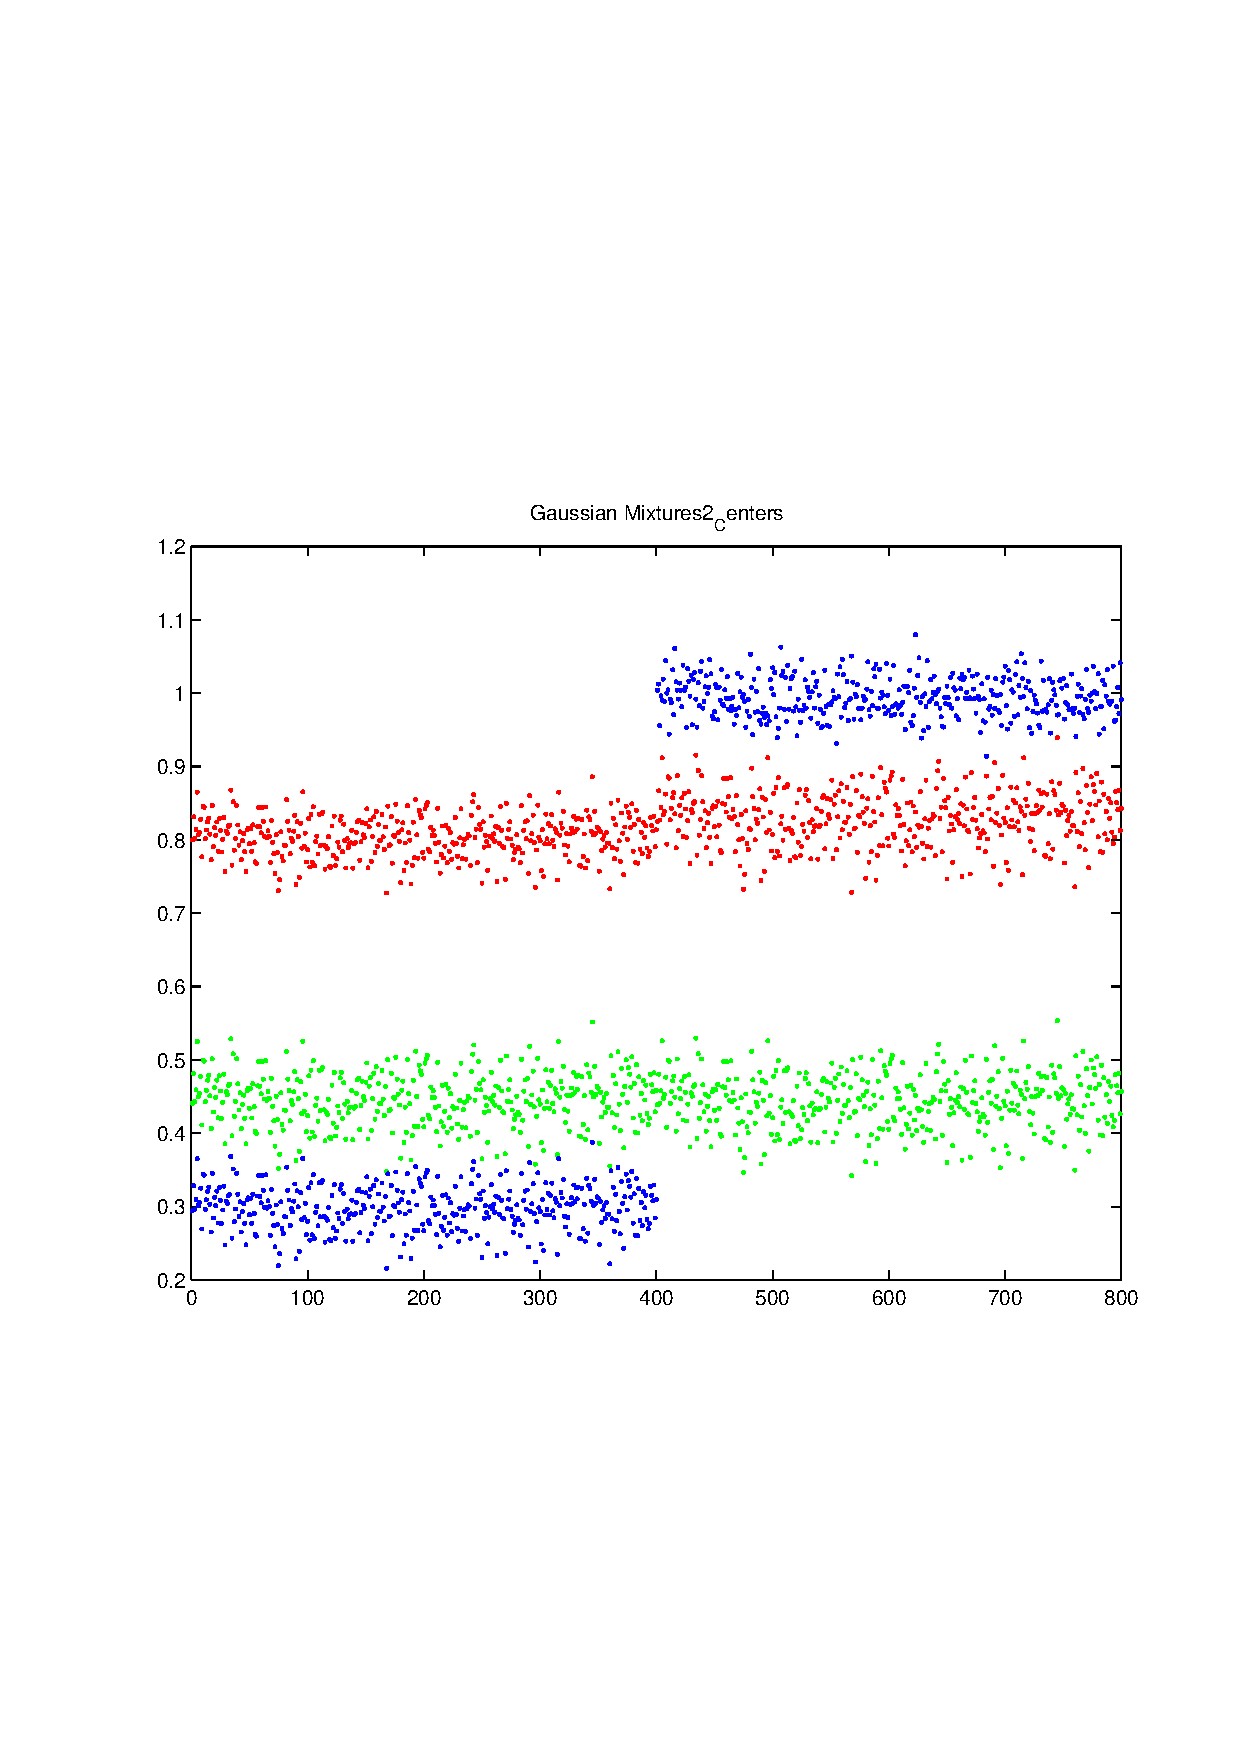
\includegraphics[width=10.0cm,height=10.0cm]{GaussianMixture_Dim_1_Centers2.pdf}

QueryPerformanceCounter  =  2.27408
\subsubsection{Matrix Quick Check <double>}
QueryPerformanceCounter  =  0.735242
\subsubsection{Matrix Quick Check <float>}
QueryPerformanceCounter  =  0.590516
\subsubsection{Intel VSL Function Check}
\includegraphics[width=10.0cm,height=10.0cm]{klVSLInv.pdf}

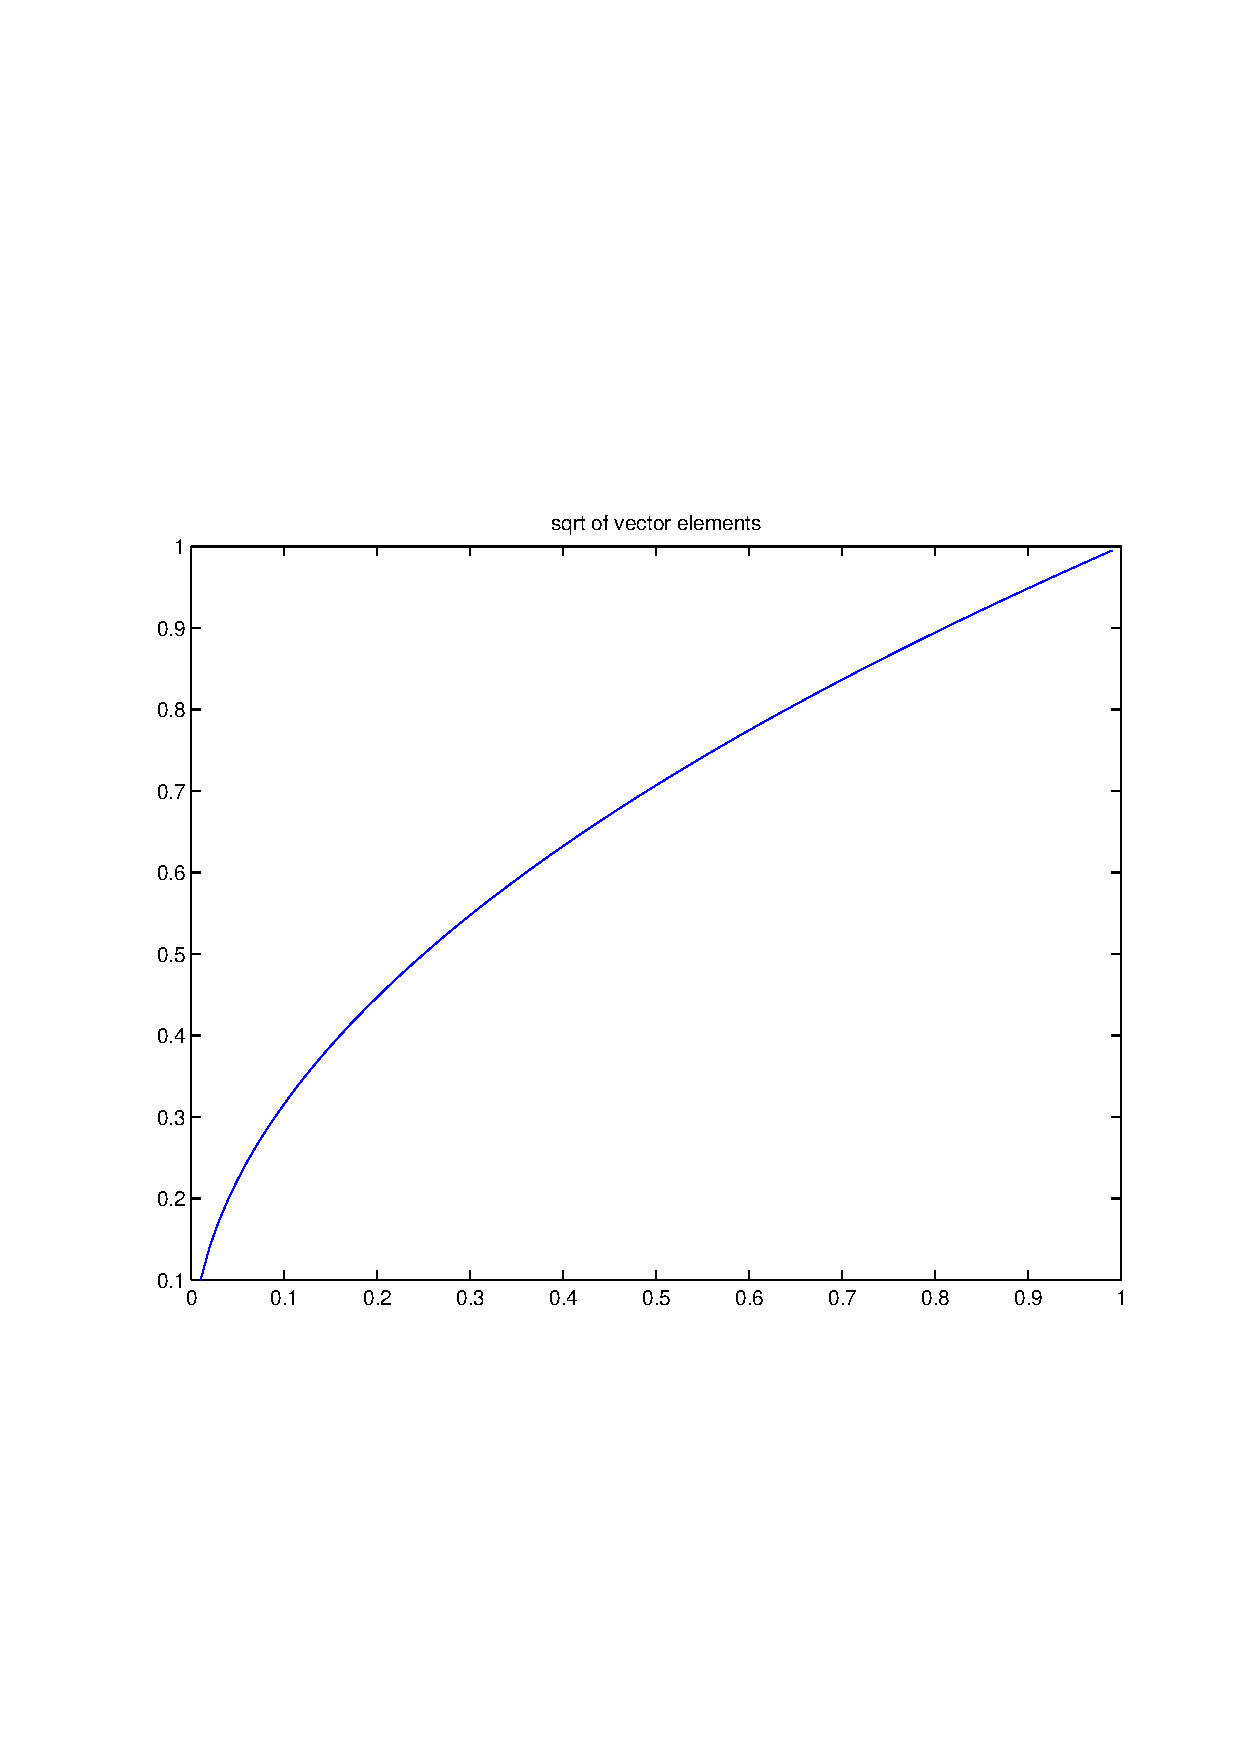
\includegraphics[width=10.0cm,height=10.0cm]{klVSLSqrt.pdf}

\includegraphics[width=10.0cm,height=10.0cm]{klVSLExp.pdf}

\includegraphics[width=10.0cm,height=10.0cm]{klVSLExpm1.pdf}

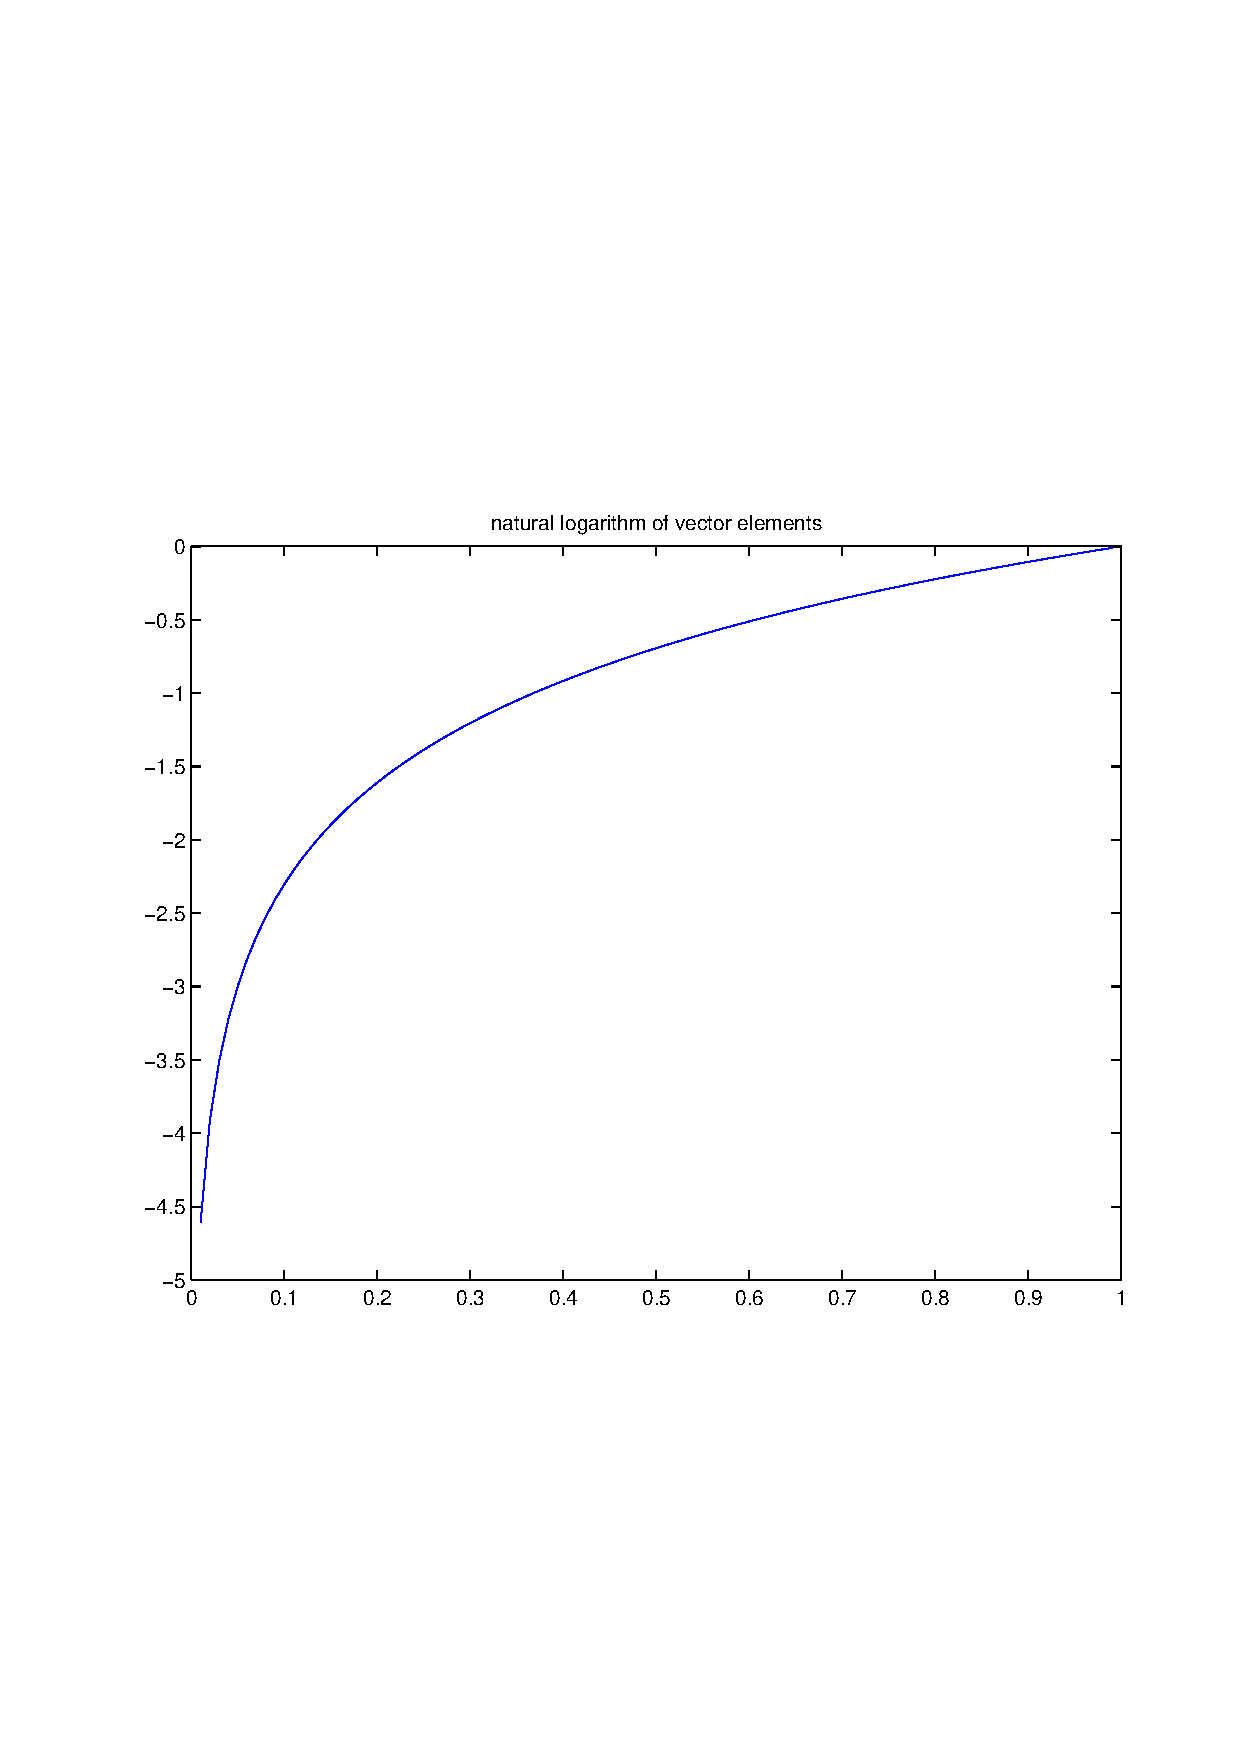
\includegraphics[width=10.0cm,height=10.0cm]{klVSLLn.pdf}

\includegraphics[width=10.0cm,height=10.0cm]{klVSLLog10.pdf}

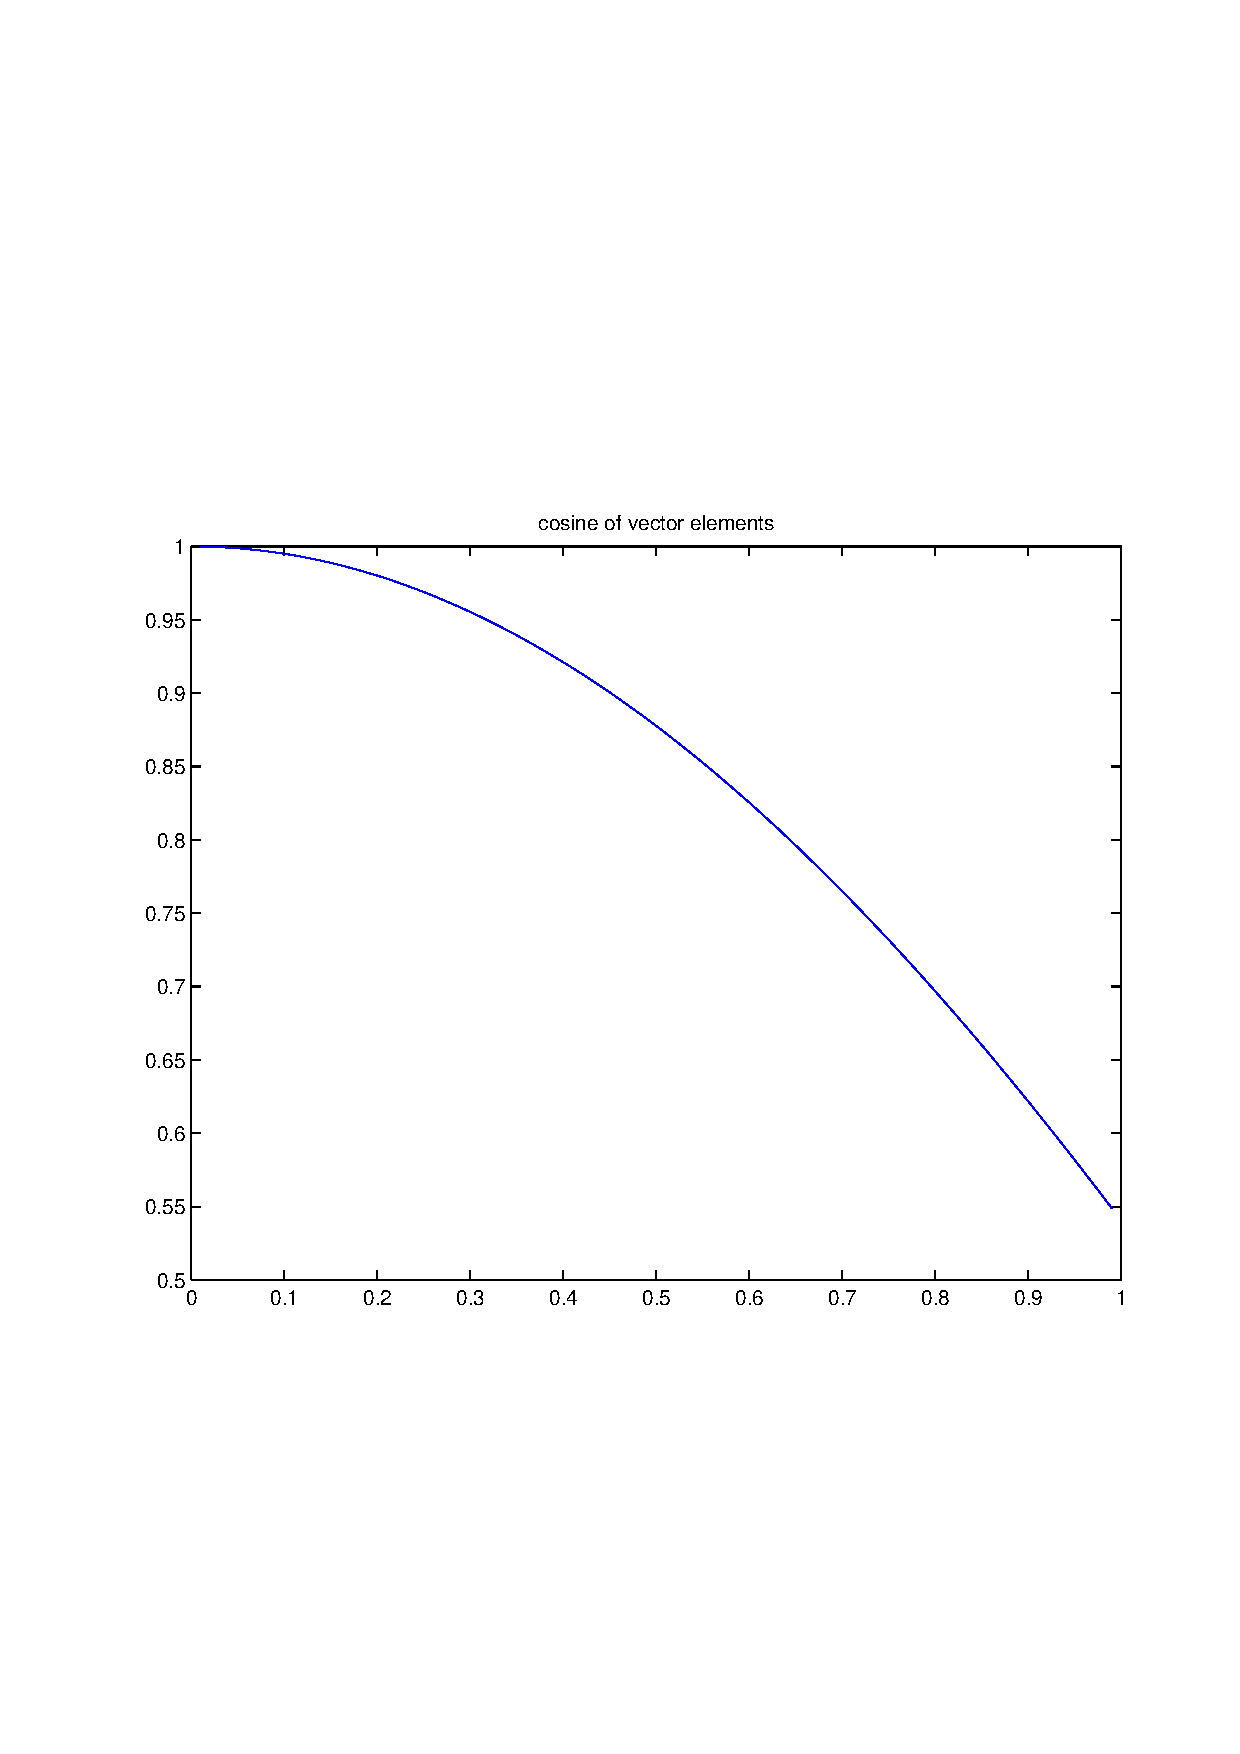
\includegraphics[width=10.0cm,height=10.0cm]{klVSLCos.pdf}

\includegraphics[width=10.0cm,height=10.0cm]{klVSLSin.pdf}

\includegraphics[width=10.0cm,height=10.0cm]{klVSLTan.pdf}

\includegraphics[width=10.0cm,height=10.0cm]{klVSLErf.pdf}

\includegraphics[width=10.0cm,height=10.0cm]{klVSLErfc.pdf}

\includegraphics[width=10.0cm,height=10.0cm]{klVSLCdfNorm.pdf}

\includegraphics[width=10.0cm,height=10.0cm]{klVSLErfInv.pdf}

\includegraphics[width=10.0cm,height=10.0cm]{klVSLLGamma.pdf}

\includegraphics[width=10.0cm,height=10.0cm]{klVSLTGamma.pdf}

QueryPerformanceCounter  =  9.95268
\subsubsection{Gram Matrix Consistency Check}
Sample Size = 4096
Feature dim = 3

$$Sigma$ = \left(
\begin{array}{
ccc}
+1.140 & +1.535 & +0.581 \\
+1.535 & +9.988 & +1.605 \\
+0.581 & +1.605 & +0.428 \\
\end{array}
\right)$ \newline 

$Sample Covariance = \left(
\begin{array}{
ccc}
+1.169 & +1.576 & +0.591 \\
+1.576 & +10.057 & +1.620 \\
+0.591 & +1.620 & +0.432 \\
\end{array}
\right)$ \newline 

$Sample Mean = \left(
\begin{array}{
ccc}
+1.02107 & +0.97126 & +1.00360 \\
\end{array}
\right)$ \newline 

$Sample Covariance-$Omega$ = \left(
\begin{array}{
ccc}
+0.029 & +0.041 & +0.010 \\
+0.041 & +0.068 & +0.014 \\
+0.010 & +0.014 & +0.004 \\
\end{array}
\right)$ \newline 

$Sample Covariance Eigs = \left(
\begin{array}{
ccc}
(+10.61086,+0.00000) & (+1.00560,+0.00000) & (+0.04130,+0.00000) \\
\end{array}
\right)$ \newline 

$Centered Mean = \left(
\begin{array}{
ccc}
-0.00000 & -0.00000 & -0.00000 \\
\end{array}
\right)$ \newline 

$Centered Covariance = \left(
\begin{array}{
ccc}
+1.169 & +1.576 & +0.591 \\
+1.576 & +10.057 & +1.620 \\
+0.591 & +1.620 & +0.432 \\
\end{array}
\right)$ \newline 

$Gram Matrix Gf Not scaled by sample size = \left(
\begin{array}{
ccc}
+4789.170 & +6453.516 & +2421.489 \\
+6453.516 & +41191.861 & +6633.169 \\
+2421.489 & +6633.169 & +1769.140 \\
\end{array}
\right)$ \newline 

$Gram Matrix Gf  scaled by sample size = \left(
\begin{array}{
ccc}
+1.169 & +1.576 & +0.591 \\
+1.576 & +10.057 & +1.619 \\
+0.591 & +1.619 & +0.432 \\
\end{array}
\right)$ \newline 

$SampleCovariance - Scaled Gf = \left(
\begin{array}{
ccc}
+0.000 & +0.000 & +0.000 \\
+0.000 & +0.002 & +0.000 \\
+0.000 & +0.000 & +0.000 \\
\end{array}
\right)$ \newline 

$EigenDecomp of SampleCovariance = \left(
\begin{array}{
ccc}
-0.172 & -0.971 & -0.165 \\
+0.919 & -0.219 & +0.329 \\
-0.356 & -0.094 & +0.930 \\
\end{array}
\right)$ \newline 

$EigenDecomp of Gram Matrix = \left(
\begin{array}{
ccc}
-0.118 & -0.975 & -0.187 \\
-0.312 & +0.215 & -0.925 \\
+0.943 & -0.051 & -0.330 \\
\end{array}
\right)$ \newline 

QueryPerformanceCounter  =  +93.152
\subsubsection{Eigen Solver Checks}
\subsubsection{Haar Distributed Random Orthogonal Matrix $A \in O(n)$}
 Testing Operator Norm
Number of Dimensions: +8

$A = \left(
\begin{array}{
cccccccc}
-0.441 & -0.310 & -0.604 & +0.297 & -0.504 & -0.016 & +0.047 & -0.007 \\
+0.565 & +0.040 & -0.380 & +0.201 & +0.118 & -0.445 & +0.530 & +0.044 \\
+0.215 & -0.652 & +0.090 & -0.113 & +0.043 & -0.041 & -0.058 & -0.708 \\
+0.410 & -0.163 & +0.141 & +0.057 & -0.441 & -0.373 & -0.585 & +0.327 \\
-0.006 & -0.296 & +0.598 & +0.228 & -0.352 & +0.144 & +0.550 & +0.235 \\
-0.159 & +0.518 & +0.271 & +0.353 & -0.278 & -0.370 & -0.014 & -0.542 \\
-0.340 & -0.055 & +0.067 & -0.695 & -0.122 & -0.570 & +0.222 & +0.074 \\
-0.363 & -0.303 & +0.164 & +0.442 & +0.565 & -0.424 & -0.137 & +0.189 \\
\end{array}
\right)$ \newline 

$Det(A) :   A \in O(n)$ = (-1.000,+0.000)

$L = \left(
\begin{array}{
cccccccc}
+1.000 & +0.000 & +0.000 & +0.000 & +0.000 & +0.000 & +0.000 & +0.000 \\
+0.381 & +1.000 & +0.000 & +0.000 & +0.000 & +0.000 & +0.000 & +0.000 \\
-0.780 & +0.417 & +1.000 & +0.000 & +0.000 & +0.000 & +0.000 & +0.000 \\
-0.603 & +0.046 & +0.173 & +1.000 & +0.000 & +0.000 & +0.000 & +0.000 \\
-0.643 & +0.416 & +0.178 & -0.846 & +1.000 & +0.000 & +0.000 & +0.000 \\
-0.010 & +0.443 & -0.492 & -0.877 & -0.729 & +1.000 & +0.000 & +0.000 \\
+0.726 & +0.288 & -0.350 & -0.231 & -0.908 & +0.917 & +1.000 & +0.000 \\
-0.282 & -0.794 & -0.351 & -0.679 & -0.514 & +0.986 & +0.602 & +1.000 \\
\end{array}
\right)$ \newline 

$U = \left(
\begin{array}{
cccccccc}
+0.565 & +0.040 & -0.380 & +0.201 & +0.118 & -0.445 & +0.530 & +0.044 \\
+0.000 & -0.667 & +0.235 & -0.190 & -0.002 & +0.129 & -0.261 & -0.724 \\
+0.000 & +0.000 & -0.998 & +0.533 & -0.411 & -0.416 & +0.570 & +0.329 \\
+0.000 & +0.000 & +0.000 & -0.657 & +0.021 & -0.772 & +0.455 & +0.077 \\
+0.000 & +0.000 & +0.000 & +0.000 & +0.733 & -1.341 & +0.595 & +0.525 \\
+0.000 & +0.000 & +0.000 & +0.000 & +0.000 & -1.776 & +1.783 & +1.167 \\
+0.000 & +0.000 & +0.000 & +0.000 & +0.000 & +0.000 & -1.686 & +0.042 \\
+0.000 & +0.000 & +0.000 & +0.000 & +0.000 & +0.000 & +0.000 & -1.845 \\
\end{array}
\right)$ \newline 

$L * U  = \left(
\begin{array}{
cccccccc}
+0.565 & +0.040 & -0.380 & +0.201 & +0.118 & -0.445 & +0.530 & +0.044 \\
+0.215 & -0.652 & +0.090 & -0.113 & +0.043 & -0.041 & -0.058 & -0.708 \\
-0.441 & -0.310 & -0.604 & +0.297 & -0.504 & -0.016 & +0.047 & -0.007 \\
-0.340 & -0.055 & +0.067 & -0.695 & -0.122 & -0.570 & +0.222 & +0.074 \\
-0.363 & -0.303 & +0.164 & +0.442 & +0.565 & -0.424 & -0.137 & +0.189 \\
-0.006 & -0.296 & +0.598 & +0.228 & -0.352 & +0.144 & +0.550 & +0.235 \\
+0.410 & -0.163 & +0.141 & +0.057 & -0.441 & -0.373 & -0.585 & +0.327 \\
-0.159 & +0.518 & +0.271 & +0.353 & -0.278 & -0.370 & -0.014 & -0.542 \\
\end{array}
\right)$ \newline 

$Det(L) :    = (+1.000,+0.000)     Det(U) :    = (+1.000,+0.000)     Det(LU) :    = (+1.000,+0.000)$

$||A||_{L_1}$  = +2.498

$||A||_{L_{\infty}}$ = +2.589

$||A^{-1}||_{L_1}$  = +2.589

$||A^{-1}||_{L_{\infty}}$ = +2.498

$||A||_{L_{\infty}} * ||A^{-1}||_{L_{\infty}} = +6.467$

$||A||_{L_1} * ||A^{-1}||_{L_1} = +6.467$

Frobenious Norm  $||A||_{\textit{F}}$ via $\sum\limits_{i,j =0}^{n} \|A_{i,j}|$   of  $A \in O(n)$  +2.828

$L_1$ condition number of Haar Distributed Random Orthogonal Matrix $A \in O(n)$ +6.018

$A = \left(
\begin{array}{
cccccccc}
-0.441 & -0.310 & -0.604 & +0.297 & -0.504 & -0.016 & +0.047 & -0.007 \\
+0.565 & +0.040 & -0.380 & +0.201 & +0.118 & -0.445 & +0.530 & +0.044 \\
+0.215 & -0.652 & +0.090 & -0.113 & +0.043 & -0.041 & -0.058 & -0.708 \\
+0.410 & -0.163 & +0.141 & +0.057 & -0.441 & -0.373 & -0.585 & +0.327 \\
-0.006 & -0.296 & +0.598 & +0.228 & -0.352 & +0.144 & +0.550 & +0.235 \\
-0.159 & +0.518 & +0.271 & +0.353 & -0.278 & -0.370 & -0.014 & -0.542 \\
-0.340 & -0.055 & +0.067 & -0.695 & -0.122 & -0.570 & +0.222 & +0.074 \\
-0.363 & -0.303 & +0.164 & +0.442 & +0.565 & -0.424 & -0.137 & +0.189 \\
\end{array}
\right)$ \newline 

$L_{\infty}$ condition number of Haar Distributed Random Orthogonal Matrix $A \in O(n)$ +6.272

Eigenvalues of $A \in O(n)$

(-0.274,+0.962), (-0.274,-0.962), (-0.761,+0.649), (-0.761,-0.649), (-1.000,+0.000), (+1.000,+0.000), (+0.753,+0.658), (+0.753,-0.658)

 $|\lambda | : \lambda \in \sigma(A) , A \in O(n)$

+1.000, +1.000, +1.000, +1.000, +1.000, +1.000, +1.000, +1.000


Calculating $A^{\dag} A,$  we expect $A^{\dag} A \approx I$

$A^{\dag} A = \left(
\begin{array}{
cccccccc}
+1.000 & -0.000 & -0.000 & -0.000 & -0.000 & -0.000 & +0.000 & +0.000 \\
-0.000 & +1.000 & +0.000 & +0.000 & -0.000 & -0.000 & -0.000 & +0.000 \\
-0.000 & +0.000 & +1.000 & +0.000 & +0.000 & -0.000 & -0.000 & +0.000 \\
-0.000 & +0.000 & +0.000 & +1.000 & -0.000 & +0.000 & +0.000 & +0.000 \\
-0.000 & -0.000 & +0.000 & -0.000 & +1.000 & +0.000 & +0.000 & +0.000 \\
-0.000 & -0.000 & -0.000 & +0.000 & +0.000 & +1.000 & -0.000 & -0.000 \\
+0.000 & -0.000 & -0.000 & +0.000 & +0.000 & -0.000 & +1.000 & +0.000 \\
+0.000 & +0.000 & +0.000 & +0.000 & +0.000 & -0.000 & +0.000 & +1.000 \\
\end{array}
\right)$ \newline 

Calculating $A^{-1} ,  A \in O(n)$.

$A^{-1} = \left(
\begin{array}{
cccccccc}
-0.441 & +0.565 & +0.215 & +0.410 & -0.006 & -0.159 & -0.340 & -0.363 \\
-0.310 & +0.040 & -0.652 & -0.163 & -0.296 & +0.518 & -0.055 & -0.303 \\
-0.604 & -0.380 & +0.090 & +0.141 & +0.598 & +0.271 & +0.067 & +0.164 \\
+0.297 & +0.201 & -0.113 & +0.057 & +0.228 & +0.353 & -0.695 & +0.442 \\
-0.504 & +0.118 & +0.043 & -0.441 & -0.352 & -0.278 & -0.122 & +0.565 \\
-0.016 & -0.445 & -0.041 & -0.373 & +0.144 & -0.370 & -0.570 & -0.424 \\
+0.047 & +0.530 & -0.058 & -0.585 & +0.550 & -0.014 & +0.222 & -0.137 \\
-0.007 & +0.044 & -0.708 & +0.327 & +0.235 & -0.542 & +0.074 & +0.189 \\
\end{array}
\right)$ \newline 

Calculating $A^{-1} *A  ,  A \in O(n)$.   We expect $A^{-1} *A  \approx I$. 

$A^{-1} *A = \left(
\begin{array}{
cccccccc}
+1.000 & +0.000 & +0.000 & +0.000 & +0.000 & +0.000 & -0.000 & +0.000 \\
-0.000 & +1.000 & +0.000 & +0.000 & +0.000 & +0.000 & -0.000 & -0.000 \\
-0.000 & -0.000 & +1.000 & -0.000 & -0.000 & -0.000 & +0.000 & +0.000 \\
+0.000 & -0.000 & +0.000 & +1.000 & -0.000 & -0.000 & +0.000 & -0.000 \\
+0.000 & -0.000 & -0.000 & -0.000 & +1.000 & -0.000 & -0.000 & +0.000 \\
-0.000 & -0.000 & -0.000 & +0.000 & +0.000 & +1.000 & +0.000 & +0.000 \\
+0.000 & +0.000 & -0.000 & -0.000 & -0.000 & -0.000 & +1.000 & +0.000 \\
+0.000 & -0.000 & -0.000 & -0.000 & +0.000 & +0.000 & +0.000 & +1.000 \\
\end{array}
\right)$ \newline 

Calculating SVD of  $A \in O(n)$

$U = \left(
\begin{array}{
cccccccc}
+0.121 & -0.089 & -0.472 & -0.489 & +0.184 & -0.373 & -0.583 & -0.054 \\
+0.768 & -0.066 & -0.326 & -0.008 & -0.254 & +0.480 & +0.056 & -0.032 \\
+0.274 & +0.105 & +0.113 & -0.074 & -0.426 & -0.641 & +0.327 & -0.444 \\
-0.266 & +0.394 & +0.189 & -0.510 & -0.567 & +0.325 & -0.225 & -0.029 \\
-0.198 & -0.256 & -0.019 & -0.174 & +0.260 & +0.337 & +0.101 & -0.821 \\
-0.441 & -0.310 & -0.604 & +0.297 & -0.504 & -0.016 & +0.047 & -0.007 \\
-0.104 & +0.728 & -0.503 & -0.014 & +0.272 & +0.024 & +0.361 & -0.047 \\
+0.073 & +0.362 & +0.067 & +0.614 & -0.055 & +0.006 & -0.597 & -0.350 \\
\end{array}
\right)$ \newline 

$S = \left(
\begin{array}{
cccccccc}
+1.000 & +0.000 & +0.000 & +0.000 & +0.000 & +0.000 & +0.000 & +0.000 \\
+0.000 & +1.000 & +0.000 & +0.000 & +0.000 & +0.000 & +0.000 & +0.000 \\
+0.000 & +0.000 & +1.000 & +0.000 & +0.000 & +0.000 & +0.000 & +0.000 \\
+0.000 & +0.000 & +0.000 & +1.000 & +0.000 & +0.000 & +0.000 & +0.000 \\
+0.000 & +0.000 & +0.000 & +0.000 & +1.000 & +0.000 & +0.000 & +0.000 \\
+0.000 & +0.000 & +0.000 & +0.000 & +0.000 & +1.000 & +0.000 & +0.000 \\
+0.000 & +0.000 & +0.000 & +0.000 & +0.000 & +0.000 & +1.000 & +0.000 \\
+0.000 & +0.000 & +0.000 & +0.000 & +0.000 & +0.000 & +0.000 & +1.000 \\
\end{array}
\right)$ \newline 

$V = \left(
\begin{array}{
cccccccc}
-0.000 & -0.000 & -0.000 & -0.000 & +0.000 & +1.000 & +0.000 & -0.000 \\
+0.022 & +0.338 & +0.490 & -0.641 & -0.251 & +0.000 & +0.370 & -0.187 \\
+0.192 & +0.169 & +0.312 & -0.244 & +0.714 & +0.000 & -0.518 & -0.004 \\
+0.351 & +0.169 & +0.197 & +0.076 & -0.620 & +0.000 & -0.588 & +0.272 \\
-0.820 & -0.000 & +0.152 & -0.002 & -0.154 & +0.000 & -0.423 & -0.318 \\
-0.242 & -0.338 & +0.607 & +0.174 & +0.079 & +0.000 & +0.189 & +0.622 \\
+0.329 & -0.507 & +0.416 & +0.268 & -0.061 & +0.000 & +0.001 & -0.621 \\
+0.021 & -0.676 & -0.244 & -0.650 & -0.096 & +0.000 & -0.187 & +0.129 \\
\end{array}
\right)$ \newline 

$U S V = \left(
\begin{array}{
cccccccc}
-0.518 & +0.266 & -0.715 & -0.051 & -0.029 & +0.121 & +0.360 & -0.050 \\
+0.043 & -0.248 & +0.148 & +0.241 & -0.135 & +0.768 & +0.353 & +0.352 \\
+0.601 & +0.393 & -0.137 & +0.165 & +0.137 & +0.274 & +0.166 & -0.563 \\
+0.178 & +0.102 & +0.176 & -0.321 & +0.482 & -0.266 & +0.654 & +0.305 \\
-0.349 & +0.271 & +0.321 & +0.774 & +0.217 & -0.198 & +0.124 & -0.041 \\
+0.414 & -0.171 & -0.346 & +0.383 & -0.463 & -0.441 & +0.235 & +0.262 \\
-0.197 & -0.001 & +0.414 & -0.214 & -0.591 & -0.104 & +0.436 & -0.440 \\
+0.076 & +0.775 & +0.151 & -0.133 & -0.345 & +0.073 & -0.172 & +0.446 \\
\end{array}
\right)$ \newline 

Calculating first few eigenvectors of $A \in O(n)$ using LAPACK syevx

\subsubsection{Wishart Matrix $A \in W(n)$}
$L_1$ condition number of Wishart Matrix +1489.694
$L_infty$ condition number of Wishart Matrix +1489.694
\subsubsection{Gaussian Orthogonal Ensemble $A \in GOE(n)$}
$L_1$ condition number of GOE Matrix +66.900
$L_\infty$ condition number of GOE Matrix +66.900
\subsubsection{The Identity Matrix $I \in M(n)$}
$L_1$ condition number of $I$ = +1.000
$L_\infty$ condition number of $I$ = +1.000
QueryPerformanceCounter  =  +1.554
\subsubsection{Generate Tracey Widom Sample}
\subsubsection{Sample from $W_n m$ times and calculate empirical PDF of the first eig}
Here we generate histograms of $\lambda_1$ for GOE (Gaussian Orthogonal Ensemble), and W (Wishart) 		 distributed of random matrices
These should approximate the celebrated Tracy Widom distribution.
Dimension $n = +128$

Sample size $m = 32$

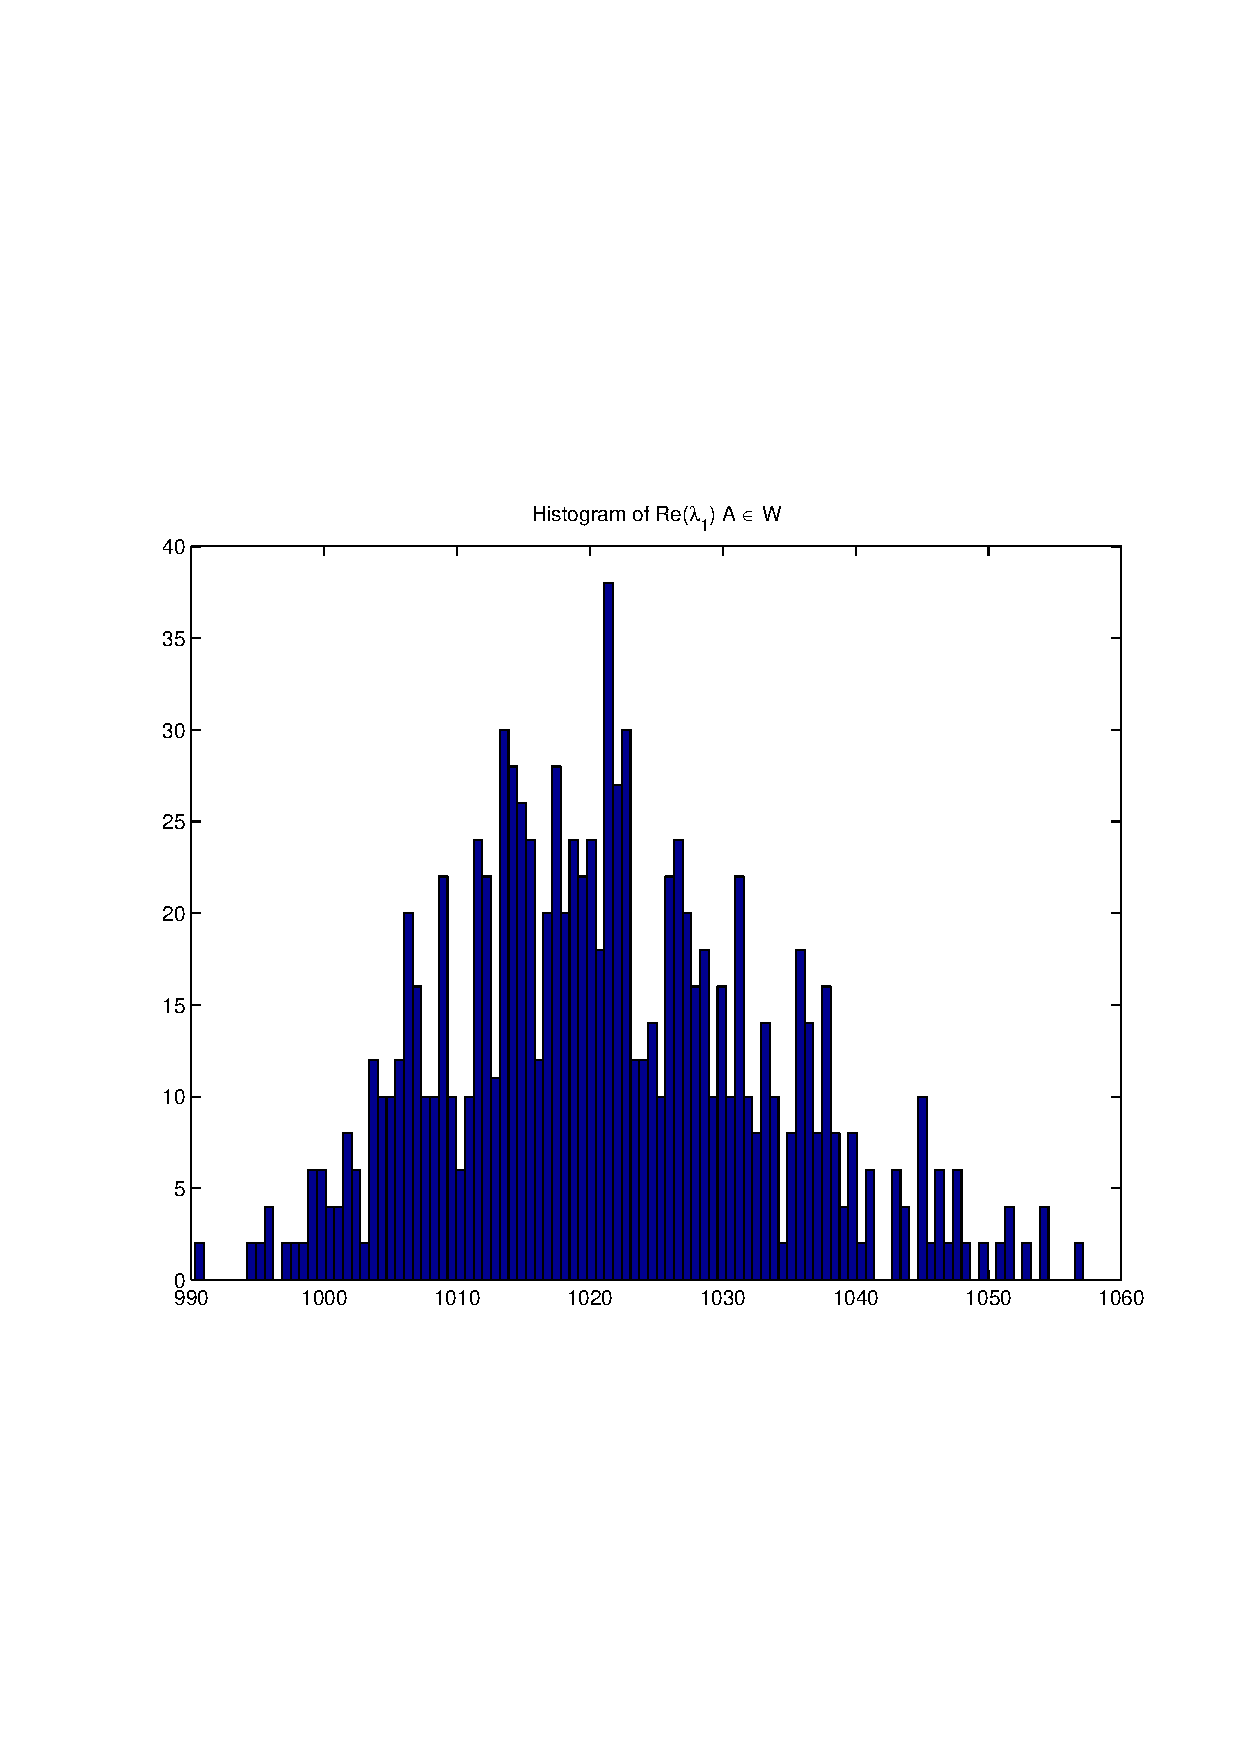
\includegraphics[width=10.0cm,height=10.0cm]{Re_TraceyWidom.pdf}

\includegraphics[width=10.0cm,height=10.0cm]{Im_TraceyWidom.pdf}

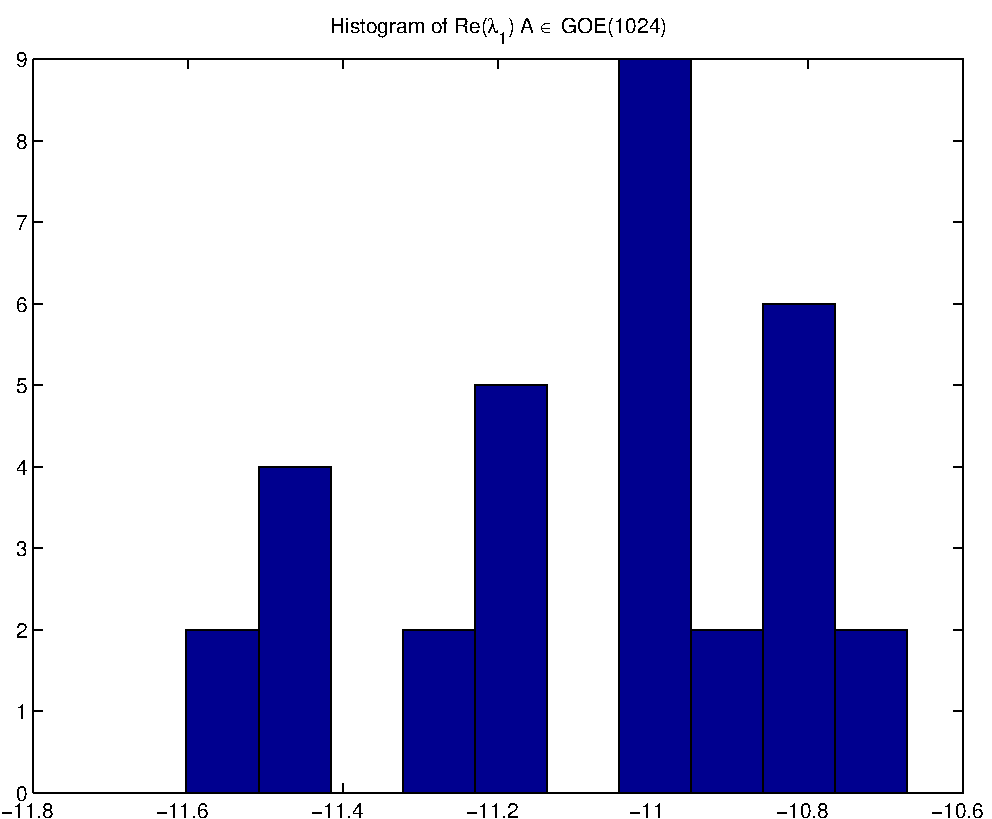
\includegraphics[width=10.0cm,height=10.0cm]{Re_Winger.pdf}

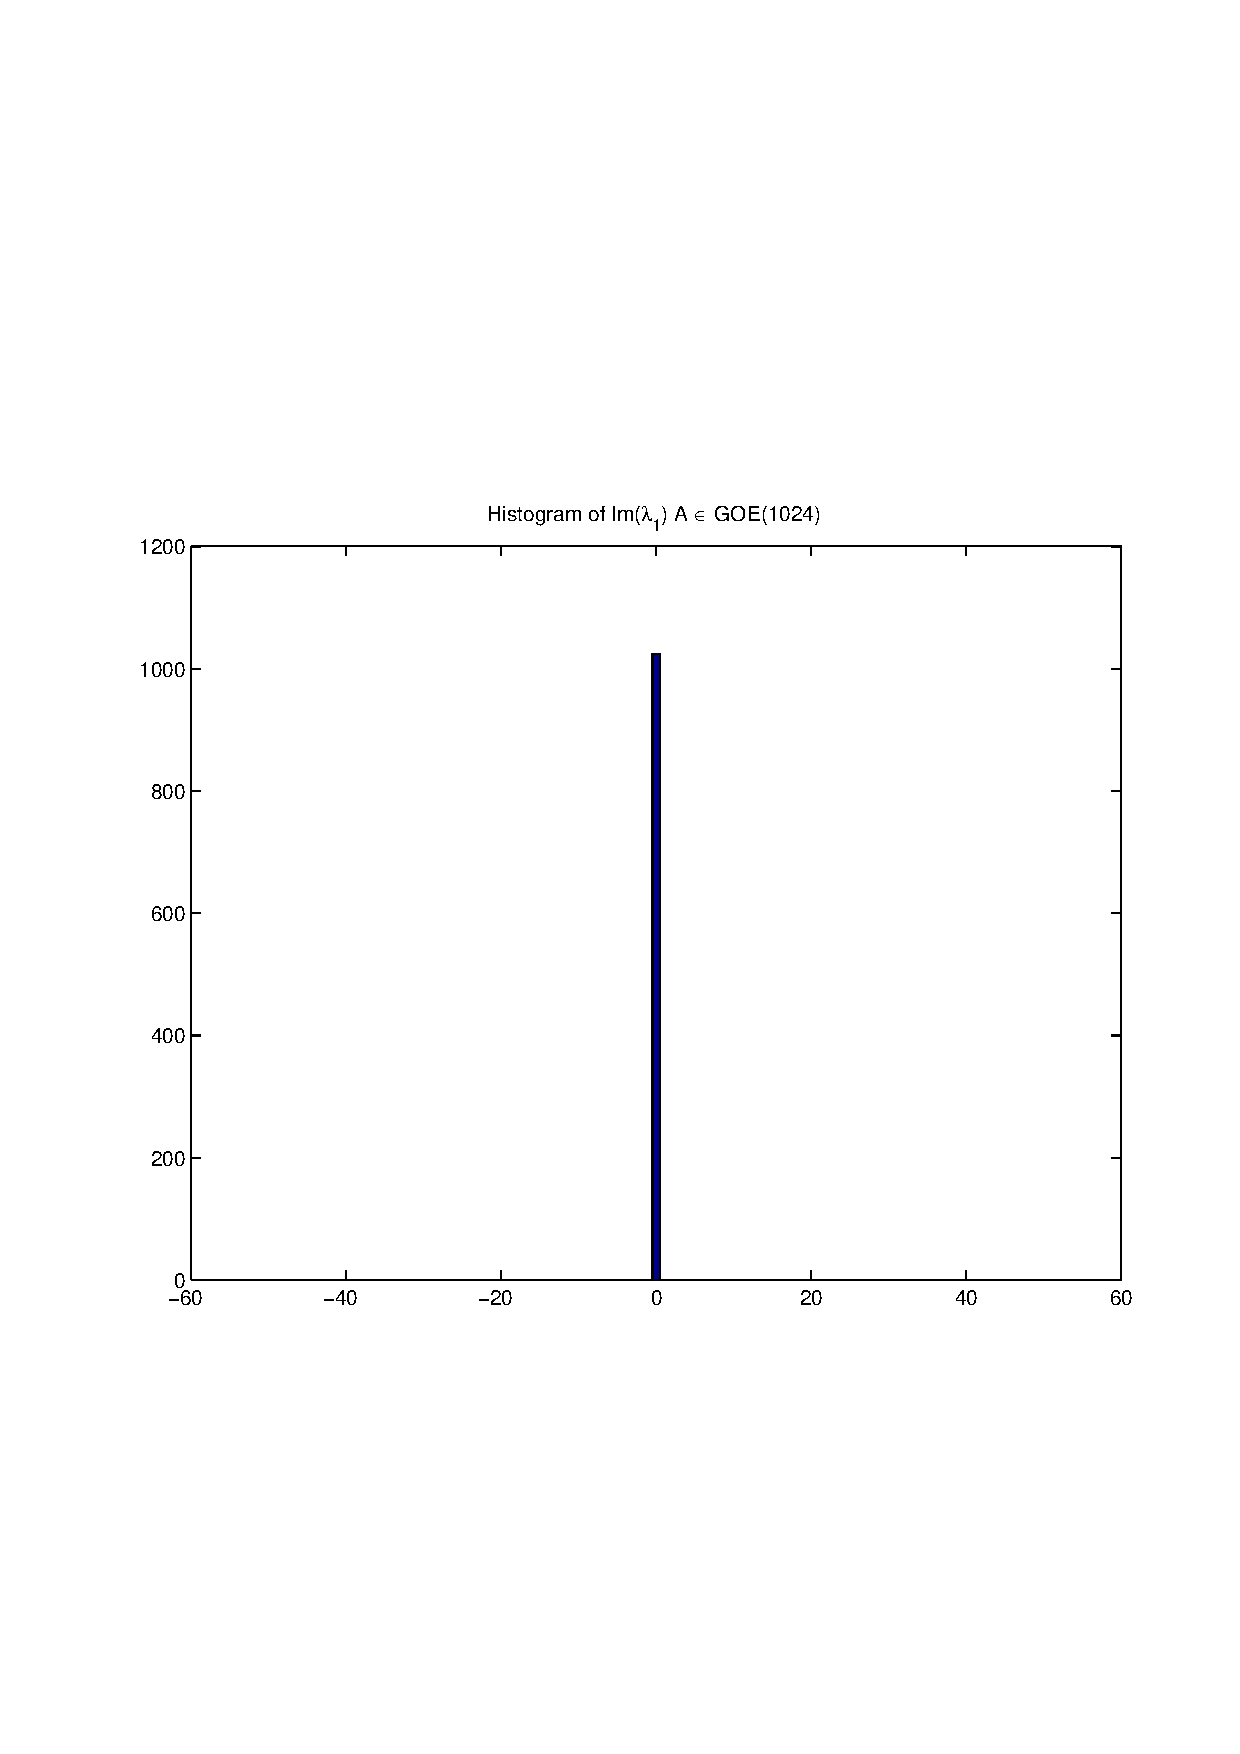
\includegraphics[width=10.0cm,height=10.0cm]{Im_Winger.pdf}

QueryPerformanceCounter  =  +5.508
\subsubsection{Approximate Winger Distribution}
\subsubsection{Verfy Winger Law.}
Let $M_n = [X_{ij} ]$ a symmetric n x n matrix with Random entries such that $X_{i,j} = X_{j,i}$, 		  and $X_{i,j}$ are iid $orall i < j,$ and $Xjj$ are iid $orall j  :  ; E[X^2_{ij} ] = 1, & E[X_{ij}] = 0$ 		  and that all moments exists for each of the entries.  		  The eigenvector of this random matrix; $ lambda_1 leq ... leq lambda_n$ depends continuously on $Mn$.
Dimension $n = +512$

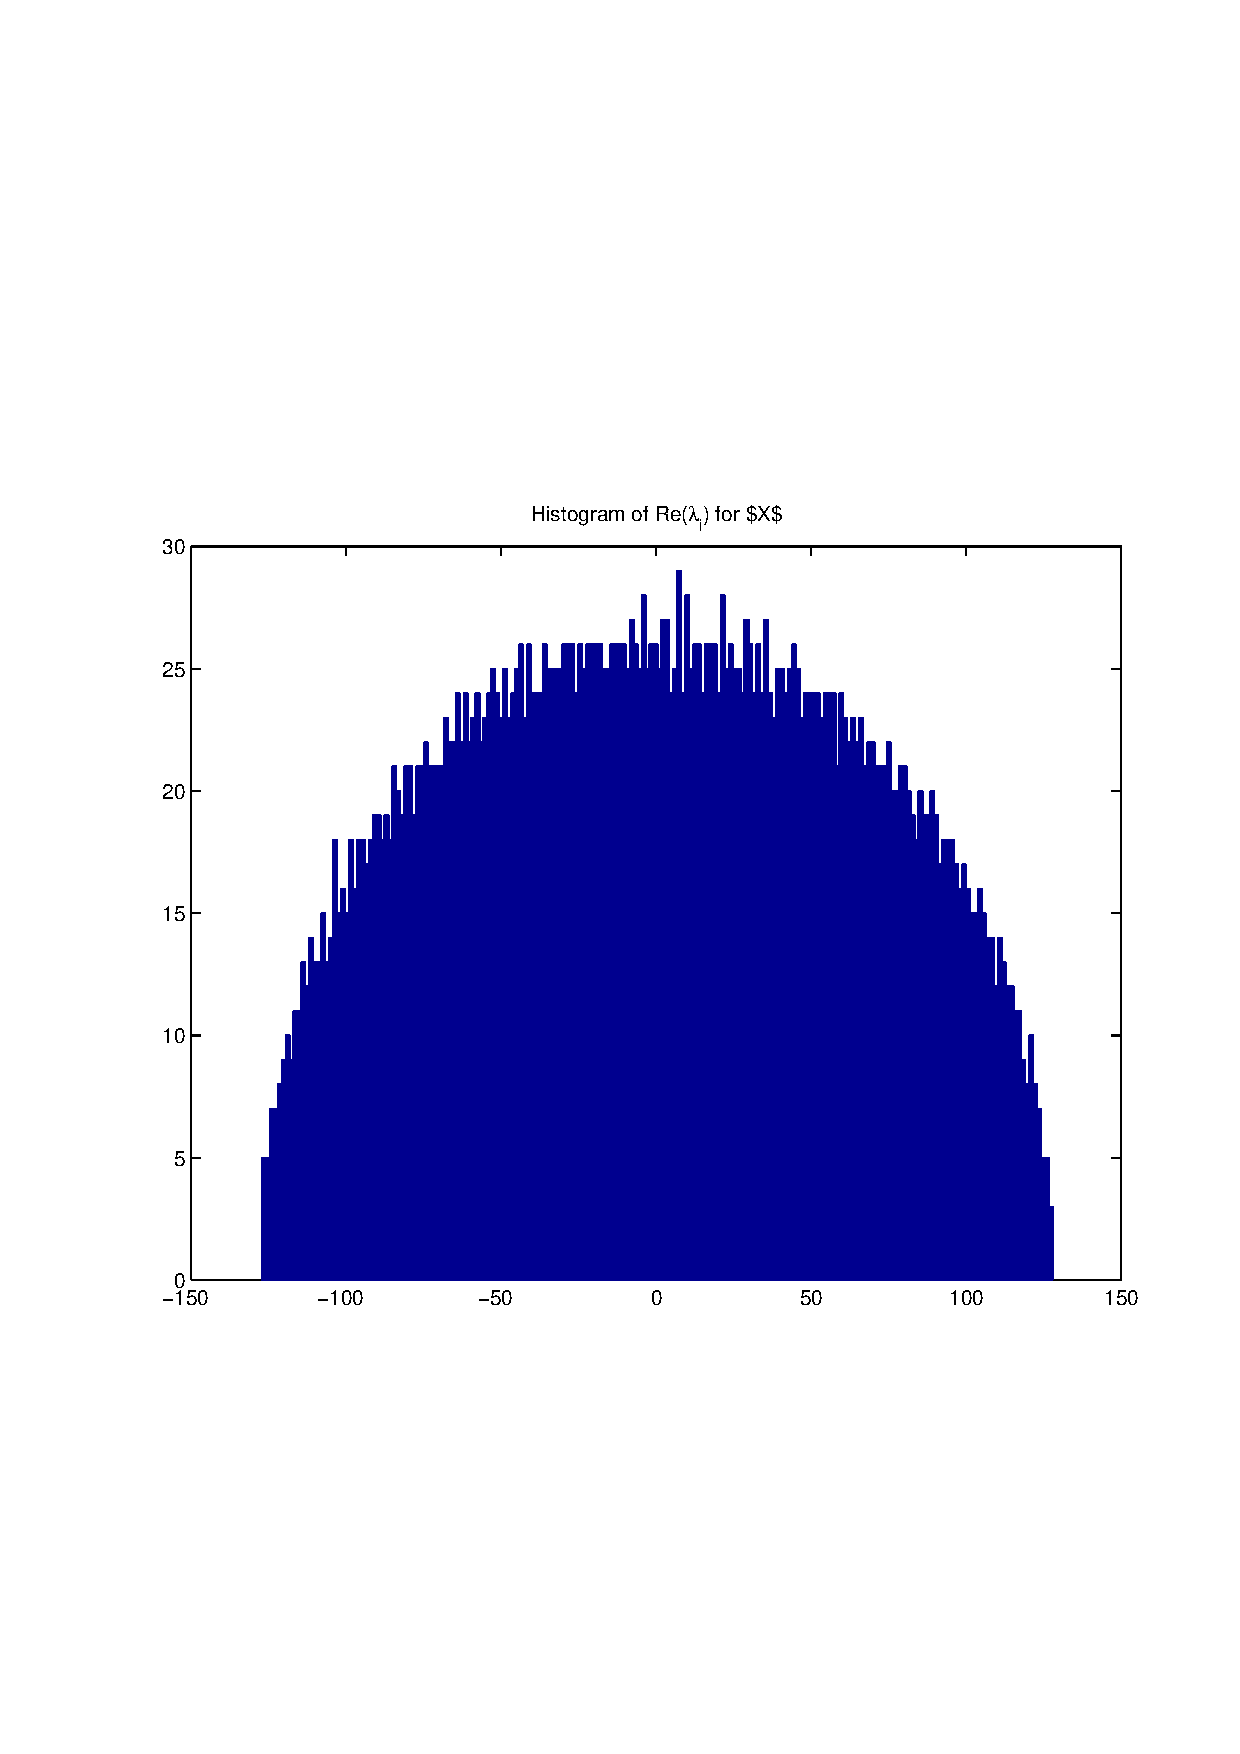
\includegraphics[width=10.0cm,height=10.0cm]{Re_lambda_n.pdf}

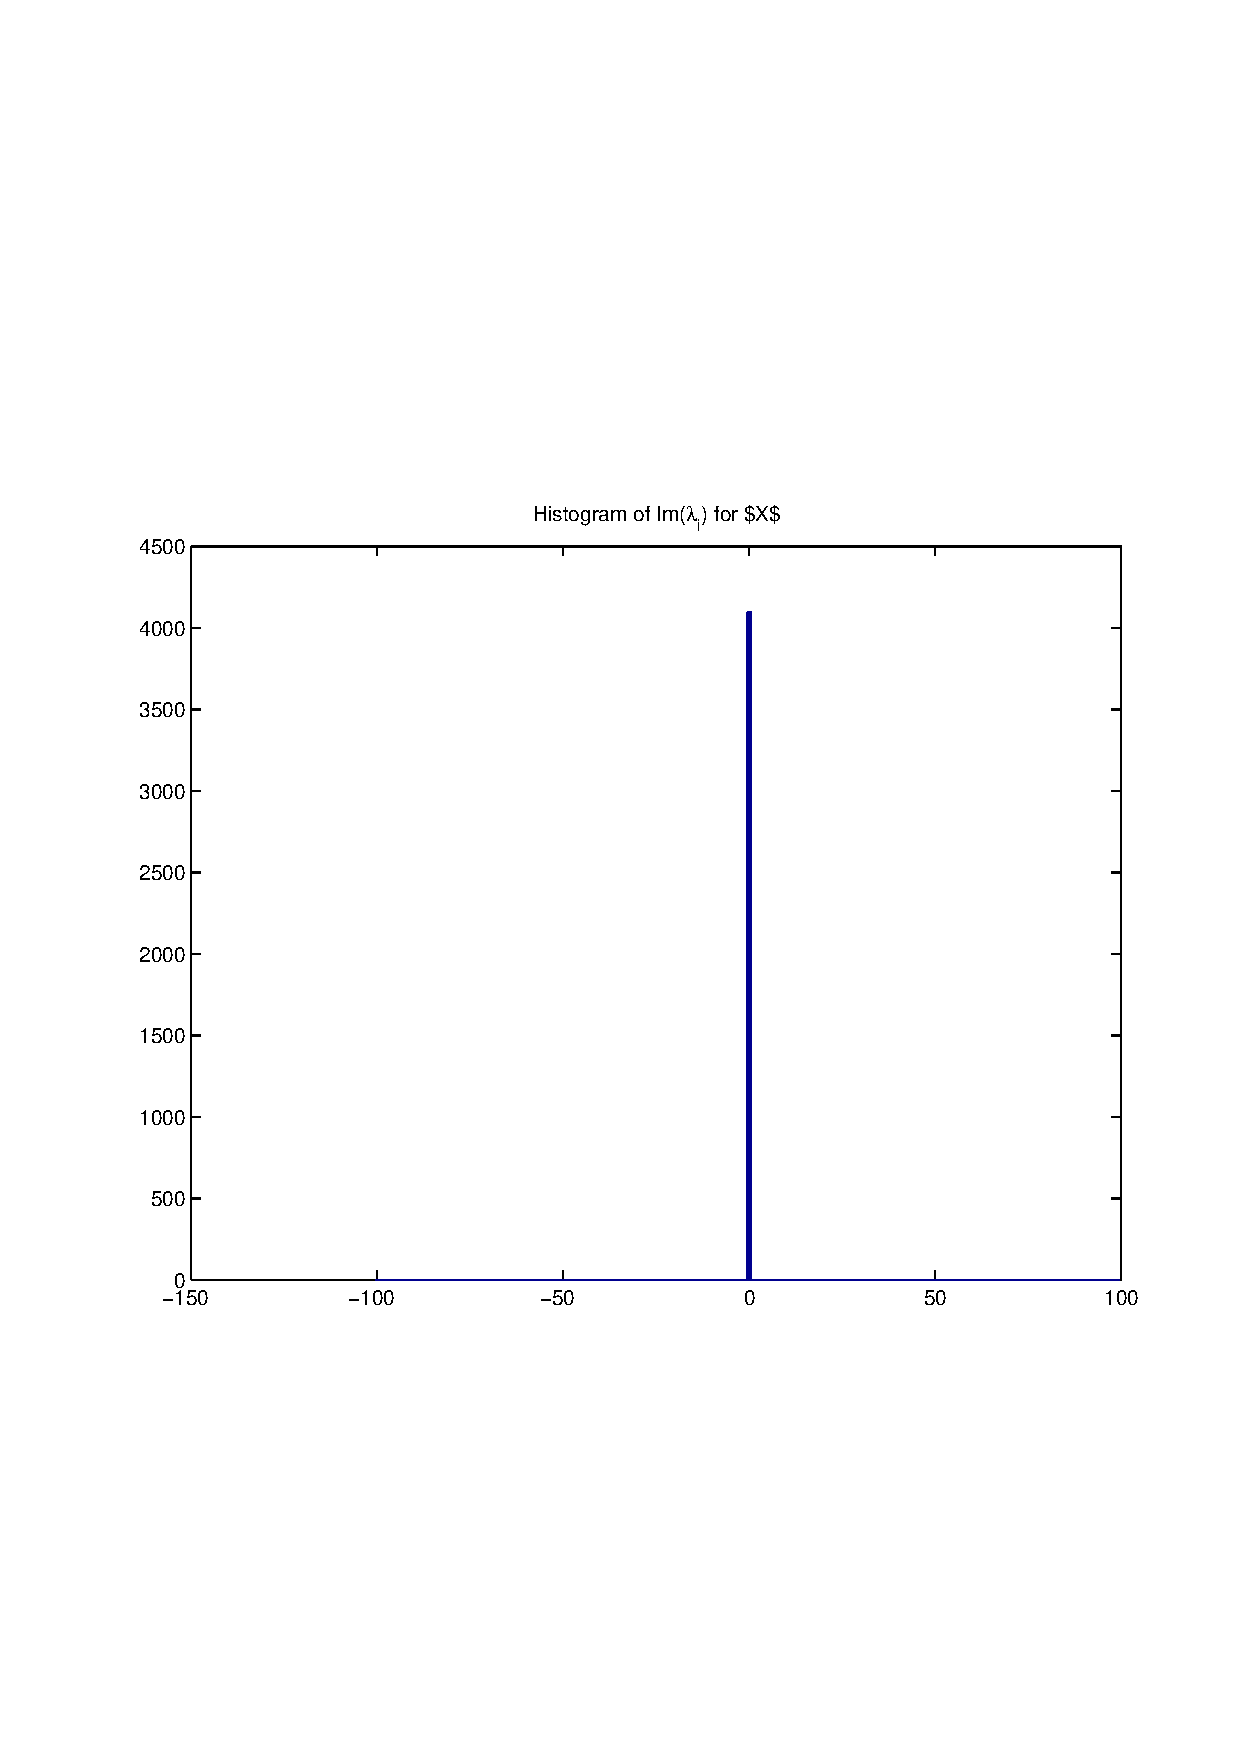
\includegraphics[width=10.0cm,height=10.0cm]{Im_lambda_n.pdf}

QueryPerformanceCounter  =  +1.905
\subsubsection{Iterated Exponential Filtering }
$\mu_1 =+0.093$
$\mu_2 =+0.726$
$\mu_3 =+0.011$
$\mu_4 =+2.178$
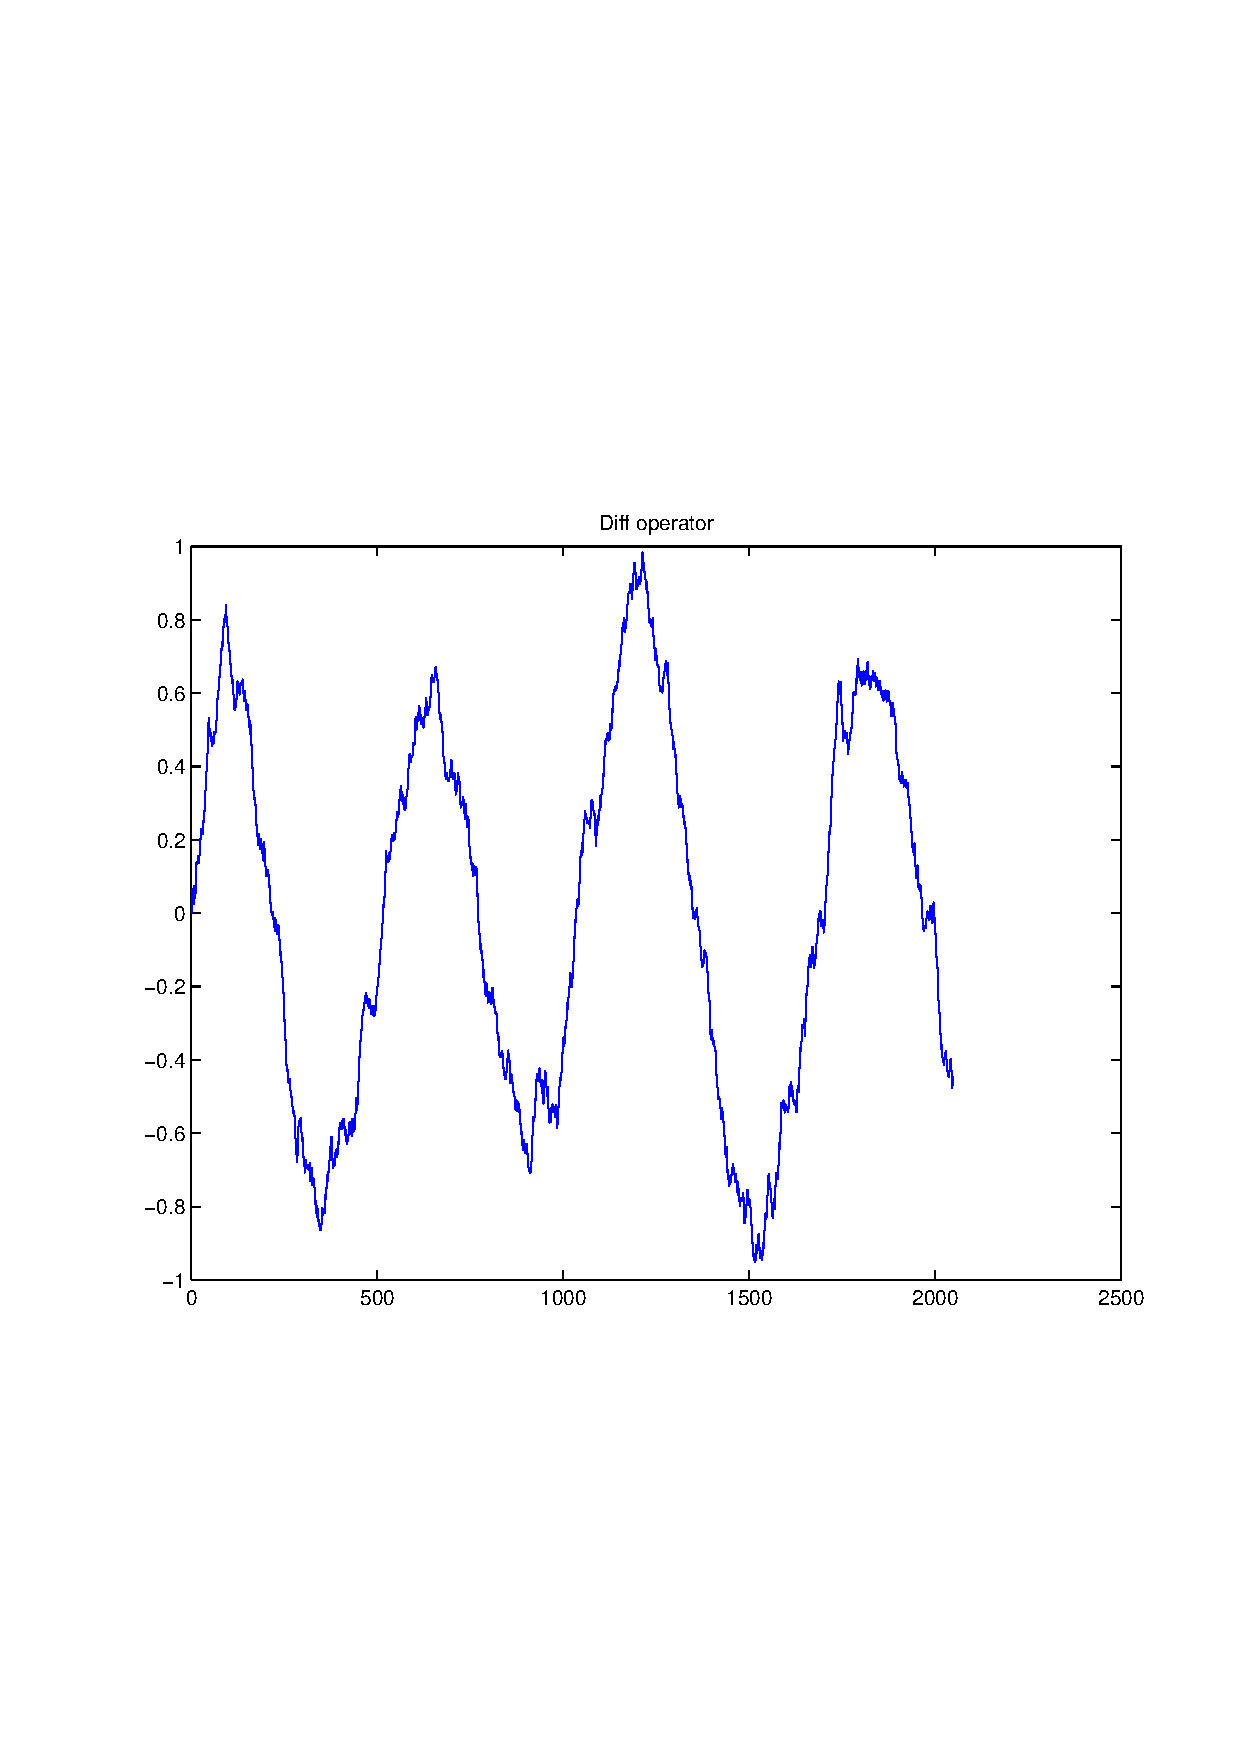
\includegraphics[width=10.0cm,height=10.0cm]{DIFF.pdf}

QueryPerformanceCounter  =  +0.856
\subsubsection{Matrix Exponential }
$SPD Matrix = \left(
\begin{array}{
cccccccc}
+10.539 & -0.499 & -0.010 & +0.368 & +0.465 & -0.492 & -0.126 & +0.437 \\
-0.499 & +7.286 & +0.365 & -0.481 & -0.337 & -0.466 & +0.279 & +0.056 \\
-0.010 & +0.365 & +6.705 & -0.205 & +0.467 & +0.131 & +0.077 & -0.089 \\
+0.368 & -0.481 & -0.205 & +6.496 & -0.402 & -0.209 & +0.043 & -0.041 \\
+0.465 & -0.337 & +0.467 & -0.402 & +4.578 & +0.272 & +0.289 & -0.285 \\
-0.492 & -0.466 & +0.131 & -0.209 & +0.272 & +8.181 & +0.343 & -0.244 \\
-0.126 & +0.279 & +0.077 & +0.043 & +0.289 & +0.343 & +5.938 & -0.212 \\
+0.437 & +0.056 & -0.089 & -0.041 & -0.285 & -0.244 & -0.212 & +9.691 \\
\end{array}
\right)$ \newline 

$SPD Eigs = \left(
\begin{array}{
cccccccc}
(+10.93611,+0.00000) & (+9.60778,+0.00000) & (+4.23666,+0.00000) & (+8.36911,+0.00000) & (+7.56229,+0.00000) & (+5.82791,+0.00000) & (+6.54198,+0.00000) & (+6.33139,+0.00000) \\
\end{array}
\right)$ \newline 

$exp(SPD) = \left(
\begin{array}{
cccccccc}
+47863.969 & -6460.093 & -1078.770 & +4706.958 & +2535.224 & -8475.398 & -2406.368 & +12977.552 \\
-6460.093 & +2780.574 & +516.920 & -1069.918 & -548.083 & -109.707 & +386.466 & -807.216 \\
-1078.770 & +516.920 & +1015.281 & -385.755 & +176.069 & +458.541 & +212.284 & -859.022 \\
+4706.958 & -1069.918 & -385.755 & +1267.210 & +111.181 & -1018.272 & -287.809 & +1036.628 \\
+2535.224 & -548.083 & +176.069 & +111.181 & +413.265 & +135.193 & +45.490 & -502.411 \\
-8475.398 & -109.707 & +458.541 & -1018.272 & +135.193 & +5613.026 & +968.003 & -4270.737 \\
-2406.368 & +386.466 & +212.284 & -287.809 & +45.490 & +968.003 & +632.432 & -1645.725 \\
+12977.552 & -807.216 & -859.022 & +1036.628 & -502.411 & -4270.737 & -1645.725 & +19362.944 \\
\end{array}
\right)$ \newline 

$exp(SPD) eigs = \left(
\begin{array}{
cccccccc}
(+56168.17045,+0.00000) & (+14880.07985,+0.00000) & (+4311.77579,+0.00000) & (+1924.25027,+0.00000) & (+69.17669,+0.00000) & (+339.64809,+0.00000) & (+693.66208,+0.00000) & (+561.93669,+0.00000) \\
\end{array}
\right)$ \newline 

$log(exp(SPD) eigs)  = \left(
\begin{array}{
cccccccc}
(+10.93611,+0.00000) & (+9.60778,+0.00000) & (+8.36911,+0.00000) & (+7.56229,+0.00000) & (+4.23666,+0.00000) & (+5.82791,+0.00000) & (+6.54198,+0.00000) & (+6.33139,+0.00000) \\
\end{array}
\right)$ \newline 

$exp(Id) = \left(
\begin{array}{
cccccccc}
+2.718 & +0.000 & +0.000 & +0.000 & +0.000 & +0.000 & +0.000 & +0.000 \\
+0.000 & +2.718 & +0.000 & +0.000 & +0.000 & +0.000 & +0.000 & +0.000 \\
+0.000 & +0.000 & +2.718 & +0.000 & +0.000 & +0.000 & +0.000 & +0.000 \\
+0.000 & +0.000 & +0.000 & +2.718 & +0.000 & +0.000 & +0.000 & +0.000 \\
+0.000 & +0.000 & +0.000 & +0.000 & +2.718 & +0.000 & +0.000 & +0.000 \\
+0.000 & +0.000 & +0.000 & +0.000 & +0.000 & +2.718 & +0.000 & +0.000 \\
+0.000 & +0.000 & +0.000 & +0.000 & +0.000 & +0.000 & +2.718 & +0.000 \\
+0.000 & +0.000 & +0.000 & +0.000 & +0.000 & +0.000 & +0.000 & +2.718 \\
\end{array}
\right)$ \newline 

$exp(Id) eigs = \left(
\begin{array}{
cccccccc}
(+2.71828,+0.00000) & (+2.71828,+0.00000) & (+2.71828,+0.00000) & (+2.71828,+0.00000) & (+2.71828,+0.00000) & (+2.71828,+0.00000) & (+2.71828,+0.00000) & (+2.71828,+0.00000) \\
\end{array}
\right)$ \newline 

$log(exp(Id) eigs)  = \left(
\begin{array}{
cccccccc}
(+1.00000,+0.00000) & (+1.00000,+0.00000) & (+1.00000,+0.00000) & (+1.00000,+0.00000) & (+1.00000,+0.00000) & (+1.00000,+0.00000) & (+1.00000,+0.00000) & (+1.00000,+0.00000) \\
\end{array}
\right)$ \newline 

For $n  \in  \dblz [16,128)$ we calculate  $|( SPD(n) Eigs - log(exp(SPD(n)) eigs)|_{l^2}$

$|( SPD(n) Eigs - log(exp(SPD(n)) eigs)|_{l^2} = \left(
\begin{array}{
cccccccccccccccccccccccccccccccccccccccccccccccccccccccccccccccccccccccccccccccccccccccccccccccccccccccccccccccc}
(+5.36543,+0.00000) & (+5.36543,+0.00000) & (+5.36543,+0.00000) & (+5.36543,+0.00000) & (+5.36543,+0.00000) & (+5.36543,+0.00000) & (+5.36543,+0.00000) & (+5.36543,+0.00000) & (+5.36543,+0.00000) & (+5.36543,+0.00000) & (+5.36543,+0.00000) & (+5.36543,+0.00000) & (+5.36543,+0.00000) & (+5.36543,+0.00000) & (+5.36543,+0.00000) & (+5.36543,+0.00000) & (+5.36543,+0.00000) & (+5.36543,+0.00000) & (+5.36543,+0.00000) & (+5.36543,+0.00000) & (+5.36543,+0.00000) & (+5.36543,+0.00000) & (+5.36543,+0.00000) & (+5.36543,+0.00000) & (+5.36543,+0.00000) & (+5.36543,+0.00000) & (+5.36543,+0.00000) & (+5.36543,+0.00000) & (+5.36543,+0.00000) & (+5.36543,+0.00000) & (+5.36543,+0.00000) & (+5.36543,+0.00000) & (+5.36543,+0.00000) & (+5.36543,+0.00000) & (+5.36543,+0.00000) & (+5.36543,+0.00000) & (+5.36543,+0.00000) & (+5.36543,+0.00000) & (+5.36543,+0.00000) & (+5.36543,+0.00000) & (+5.36543,+0.00000) & (+5.36543,+0.00000) & (+5.36543,+0.00000) & (+5.36543,+0.00000) & (+5.36543,+0.00000) & (+5.36543,+0.00000) & (+5.36543,+0.00000) & (+5.36543,+0.00000) & (+0.00000,+0.00000) & (+0.00000,+0.00000) & (+0.00000,+0.00000) & (+0.00000,+0.00000) & (+0.00000,+0.00000) & (+0.00000,+0.00000) & (+0.00000,+0.00000) & (+0.00000,+0.00000) & (+0.00000,+0.00000) & (+0.00000,+0.00000) & (+0.00000,+0.00000) & (+0.00000,+0.00000) & (+0.00000,+0.00000) & (+0.00000,+0.00000) & (+0.00000,+0.00000) & (+0.00000,+0.00000) & (+0.00000,+0.00000) & (+0.00000,+0.00000) & (+0.00000,+0.00000) & (+0.00000,+0.00000) & (+0.00000,+0.00000) & (+0.00000,+0.00000) & (+0.00000,+0.00000) & (+0.00000,+0.00000) & (+0.00000,+0.00000) & (+0.00000,+0.00000) & (+0.00000,+0.00000) & (+0.00000,+0.00000) & (+0.00000,+0.00000) & (+0.00000,+0.00000) & (+0.00000,+0.00000) & (+0.00000,+0.00000) & (+0.00000,+0.00000) & (+0.00000,+0.00000) & (+0.00000,+0.00000) & (+0.00000,+0.00000) & (+0.00000,+0.00000) & (+0.00000,+0.00000) & (+0.00000,+0.00000) & (+0.00000,+0.00000) & (+0.00000,+0.00000) & (+0.00000,+0.00000) & (+0.00000,+0.00000) & (+0.00000,+0.00000) & (+0.00000,+0.00000) & (+0.00000,+0.00000) & (+0.00000,+0.00000) & (+0.00000,+0.00000) & (+0.00000,+0.00000) & (+0.00000,+0.00000) & (+0.00000,+0.00000) & (+0.00000,+0.00000) & (+0.00000,+0.00000) & (+0.00000,+0.00000) & (+0.00000,+0.00000) & (+0.00000,+0.00000) & (+0.00000,+0.00000) & (+0.00000,+0.00000) & (+0.00000,+0.00000) & (+0.00000,+0.00000) & (+0.00000,+0.00000) & (+0.00000,+0.00000) & (+0.00000,+0.00000) & (+0.00000,+0.00000) \\
\end{array}
\right)$ \newline 

QueryPerformanceCounter  =  +0.02163
The sample size generated for this run is 100000.

\newpage
uniform \begin{tabular}{|c|c|c|c|}  mean & variance & skewness & kurtosis \\  \hline
$\mu_1 = +0.50030$ & $\mu_2 = +0.08353$ & $\mu_3 = +0.00339$ & $\mu_4 =+1.80113$ \\
\end{tabular}

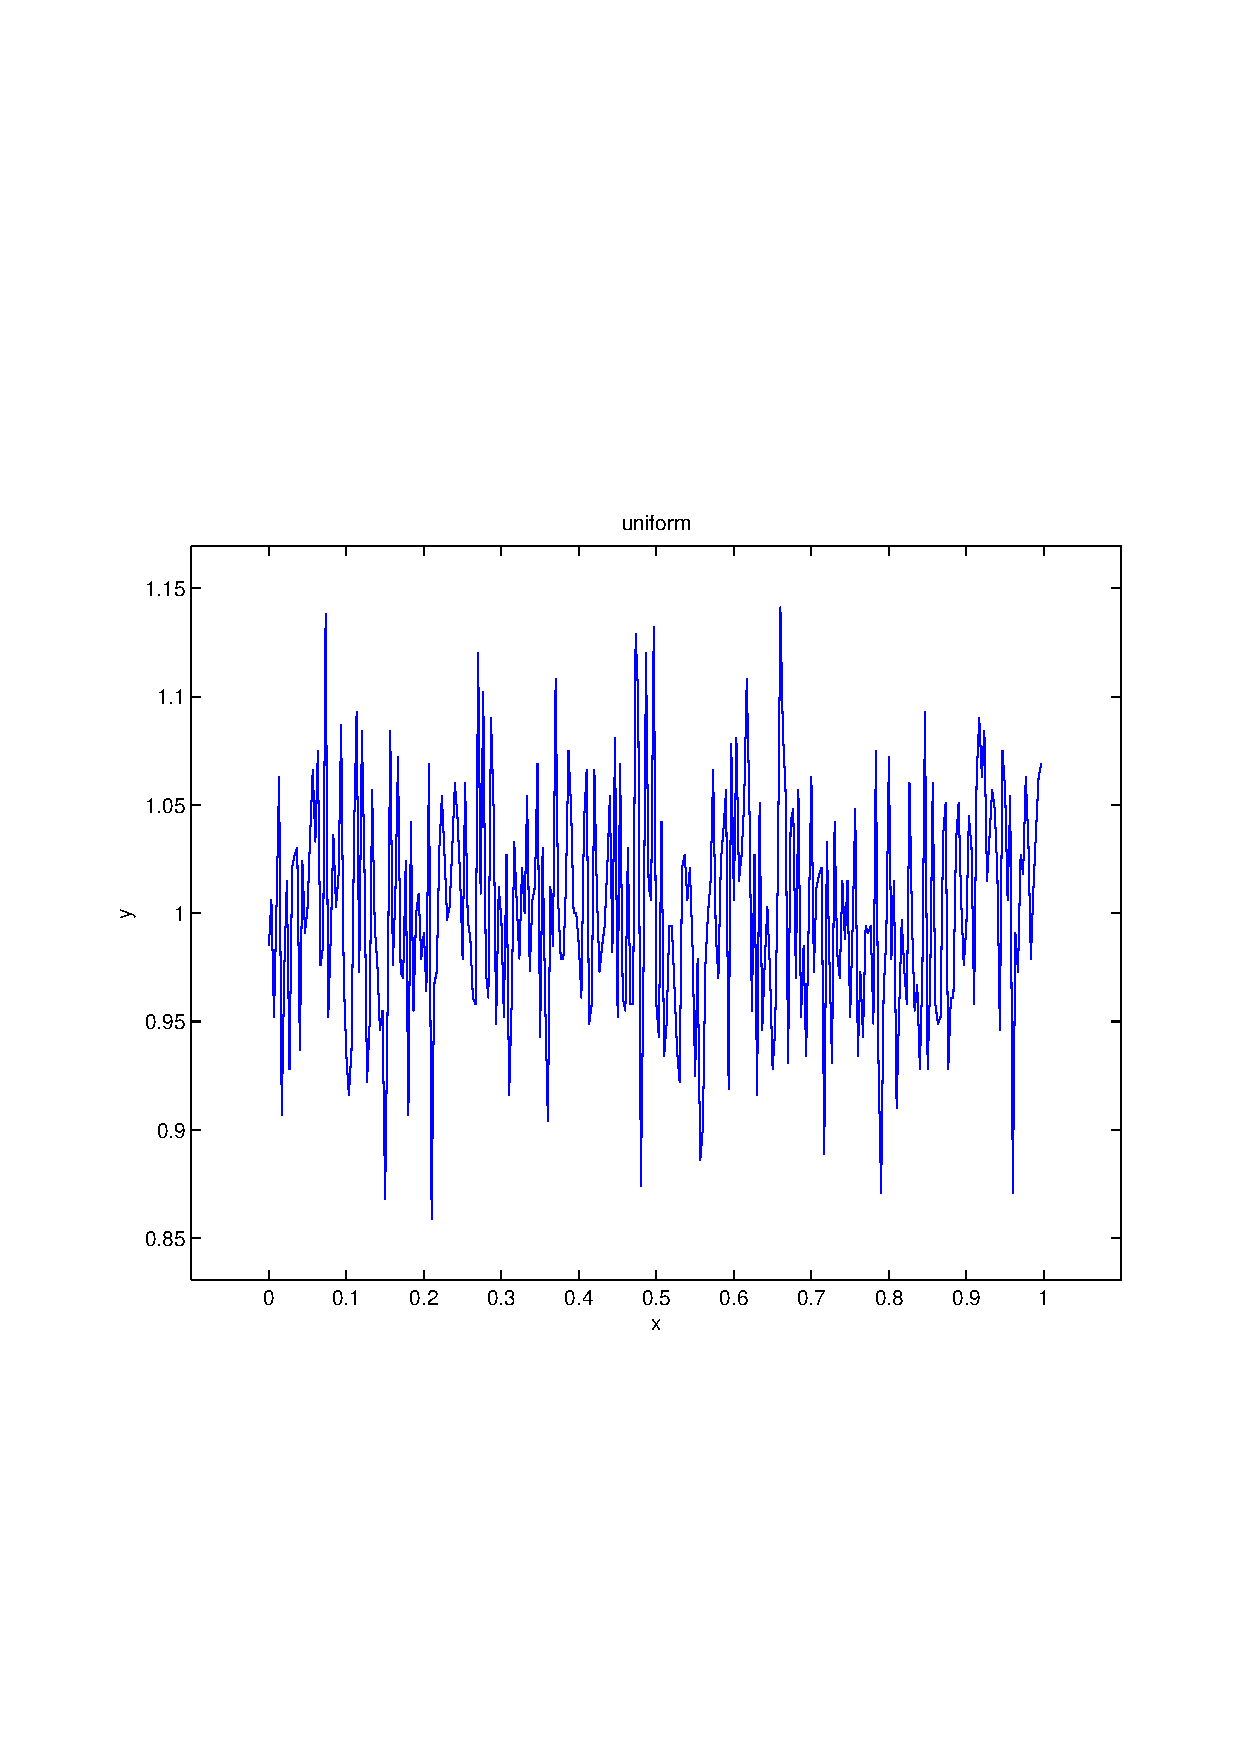
\includegraphics[width=5cm,height=5cm]{uniform.pdf}

cauchy \begin{tabular}{|c|c|c|c|}  mean & variance & skewness & kurtosis \\  \hline
$\mu_1 = +0.44288$ & $\mu_2 = +0.05341$ & $\mu_3 = +0.63935$ & $\mu_4 =+3.28094$ \\
\end{tabular}

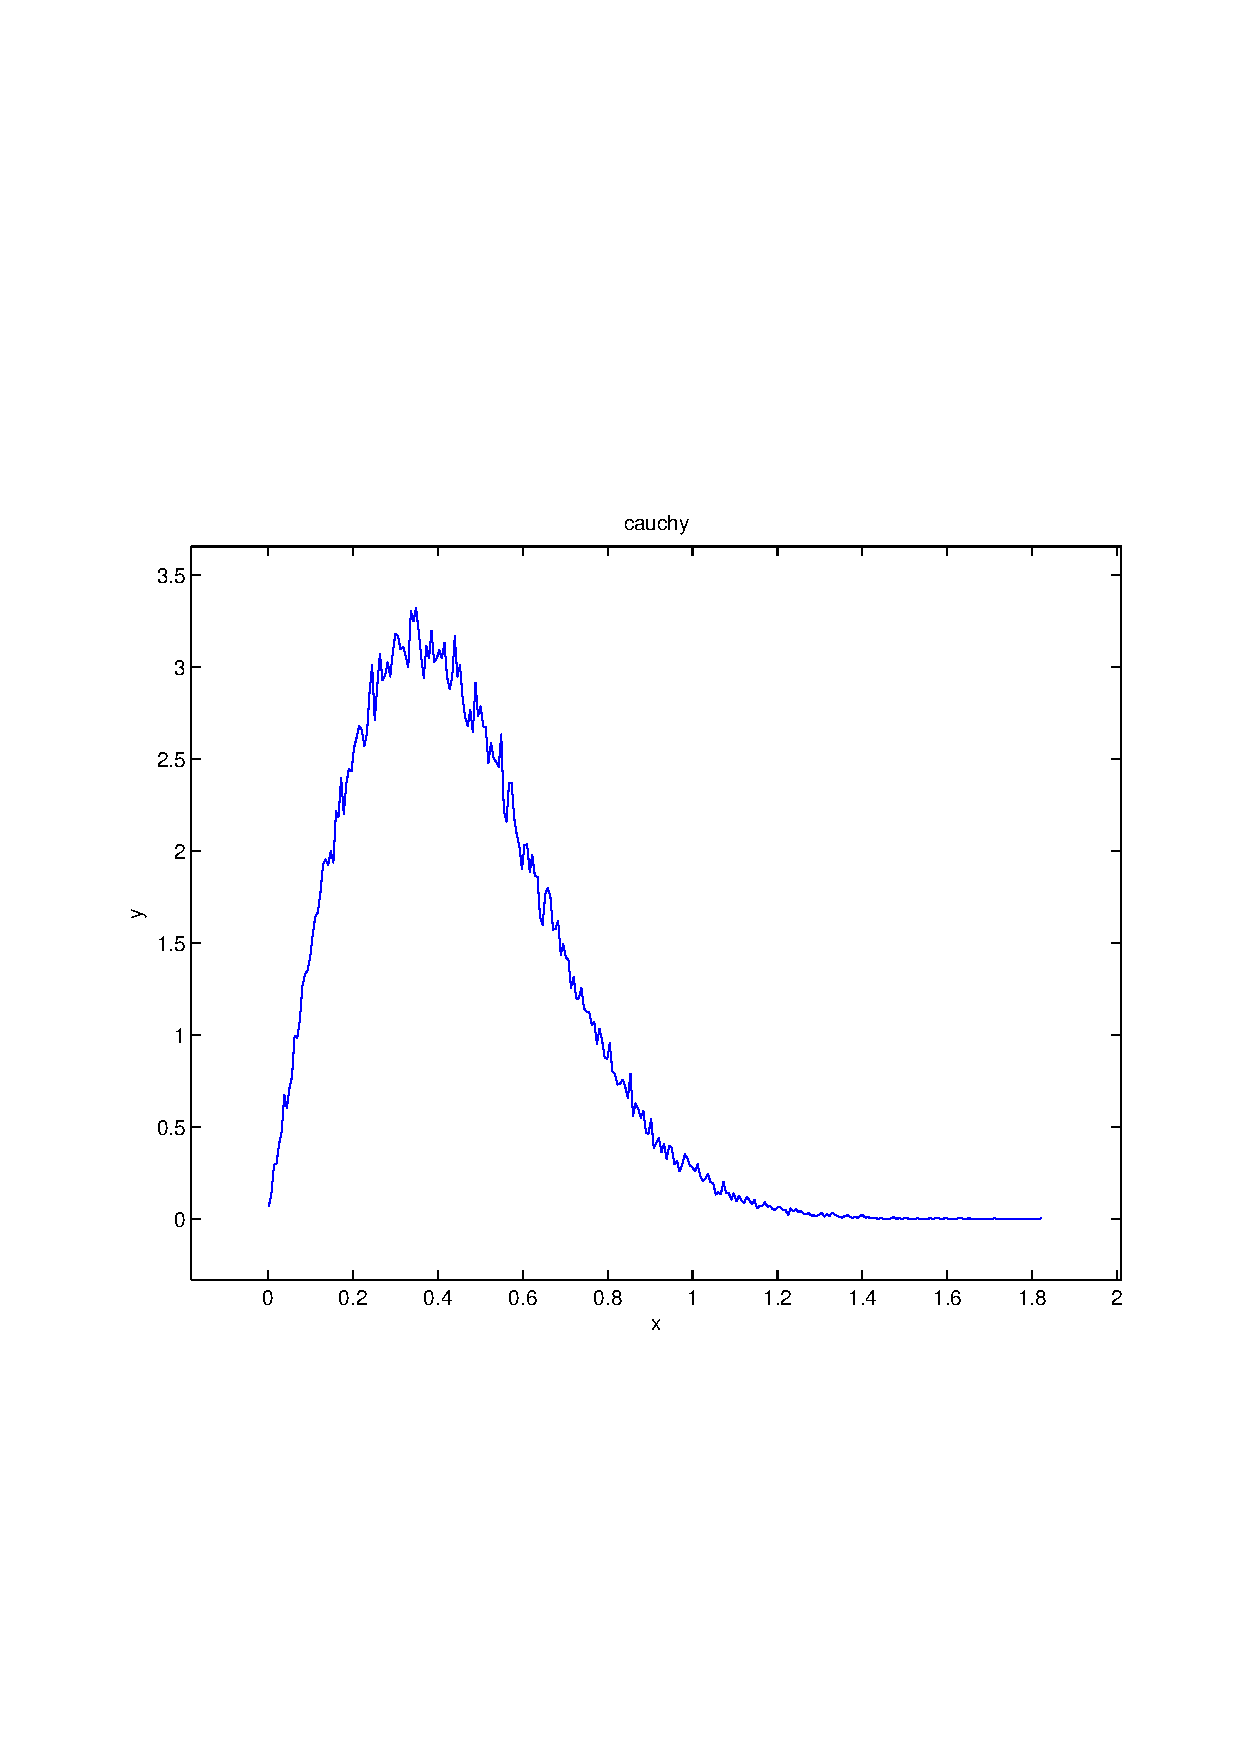
\includegraphics[width=5cm,height=5cm]{cauchy.pdf}

exponential \begin{tabular}{|c|c|c|c|}  mean & variance & skewness & kurtosis \\  \hline
$\mu_1 = +1.99647$ & $\mu_2 = +3.99339$ & $\mu_3 = +2.03097$ & $\mu_4 =+9.30842$ \\
\end{tabular}

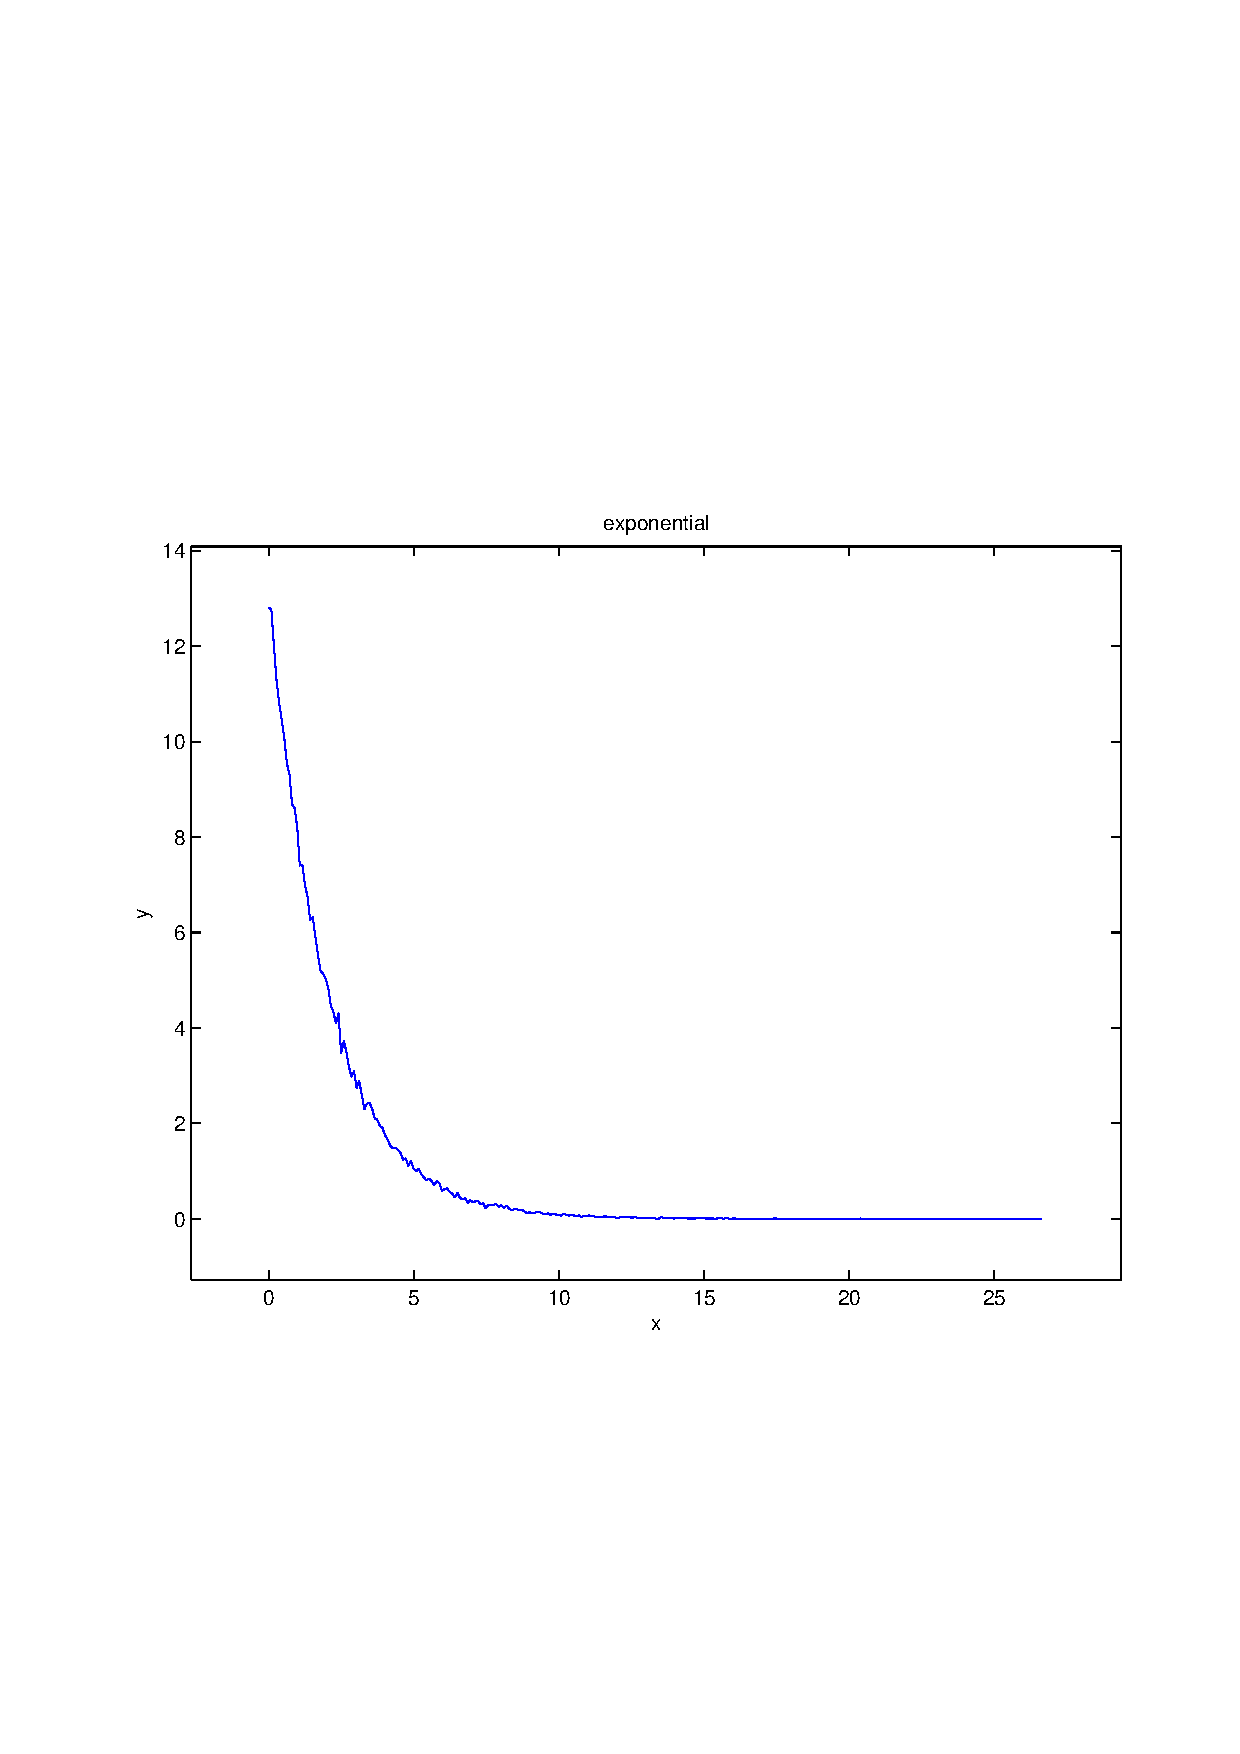
\includegraphics[width=5cm,height=5cm]{exponential.pdf}

\newpage
gamma \begin{tabular}{|c|c|c|c|}  mean & variance & skewness & kurtosis \\  \hline
$\mu_1 = +1.90706$ & $\mu_2 = +1.92833$ & $\mu_3 = +1.44894$ & $\mu_4 =+6.13430$ \\
\end{tabular}

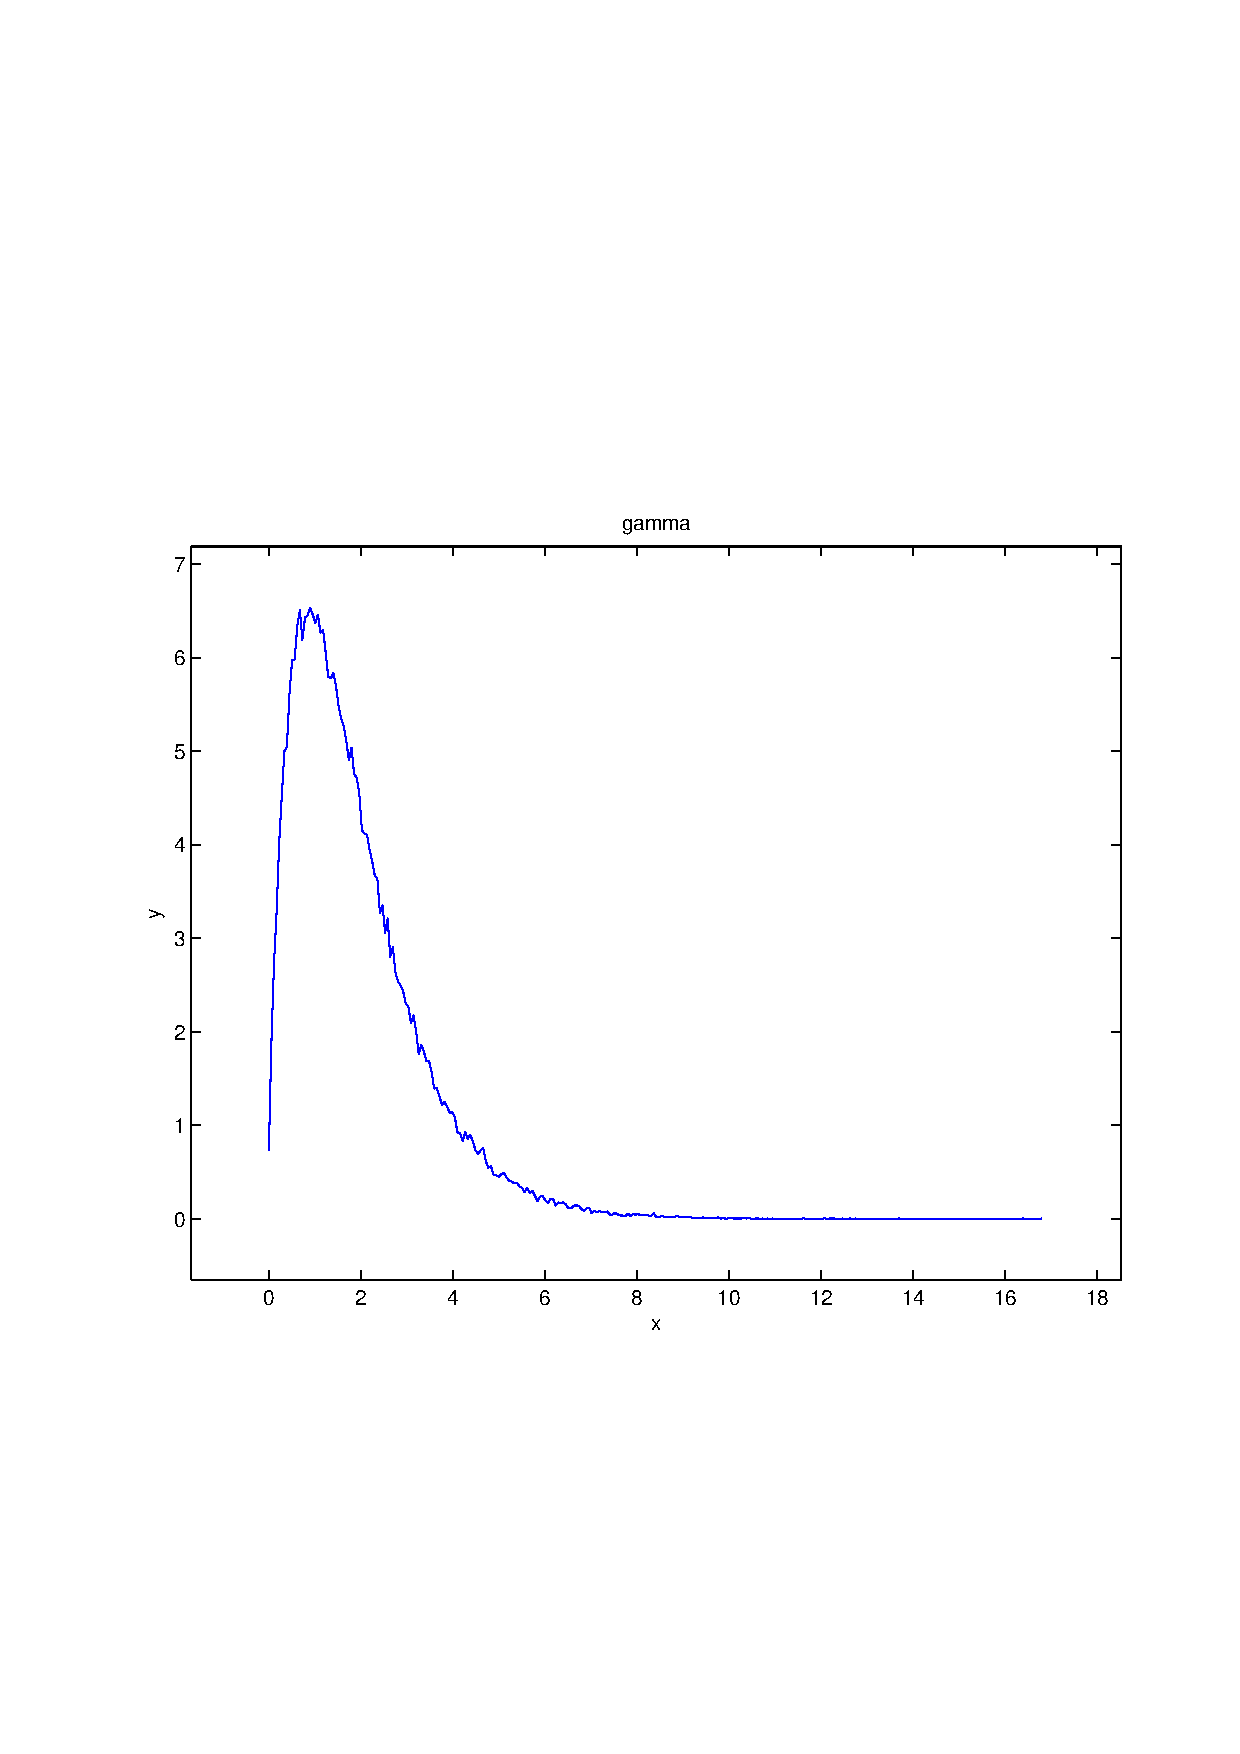
\includegraphics[width=5cm,height=5cm]{gamma.pdf}

GIG \begin{tabular}{|c|c|c|c|}  mean & variance & skewness & kurtosis \\  \hline
$\mu_1 = +0.81043$ & $\mu_2 = +11.68253$ & $\mu_3 = +15.18063$ & $\mu_4 =+303.36105$ \\
\end{tabular}

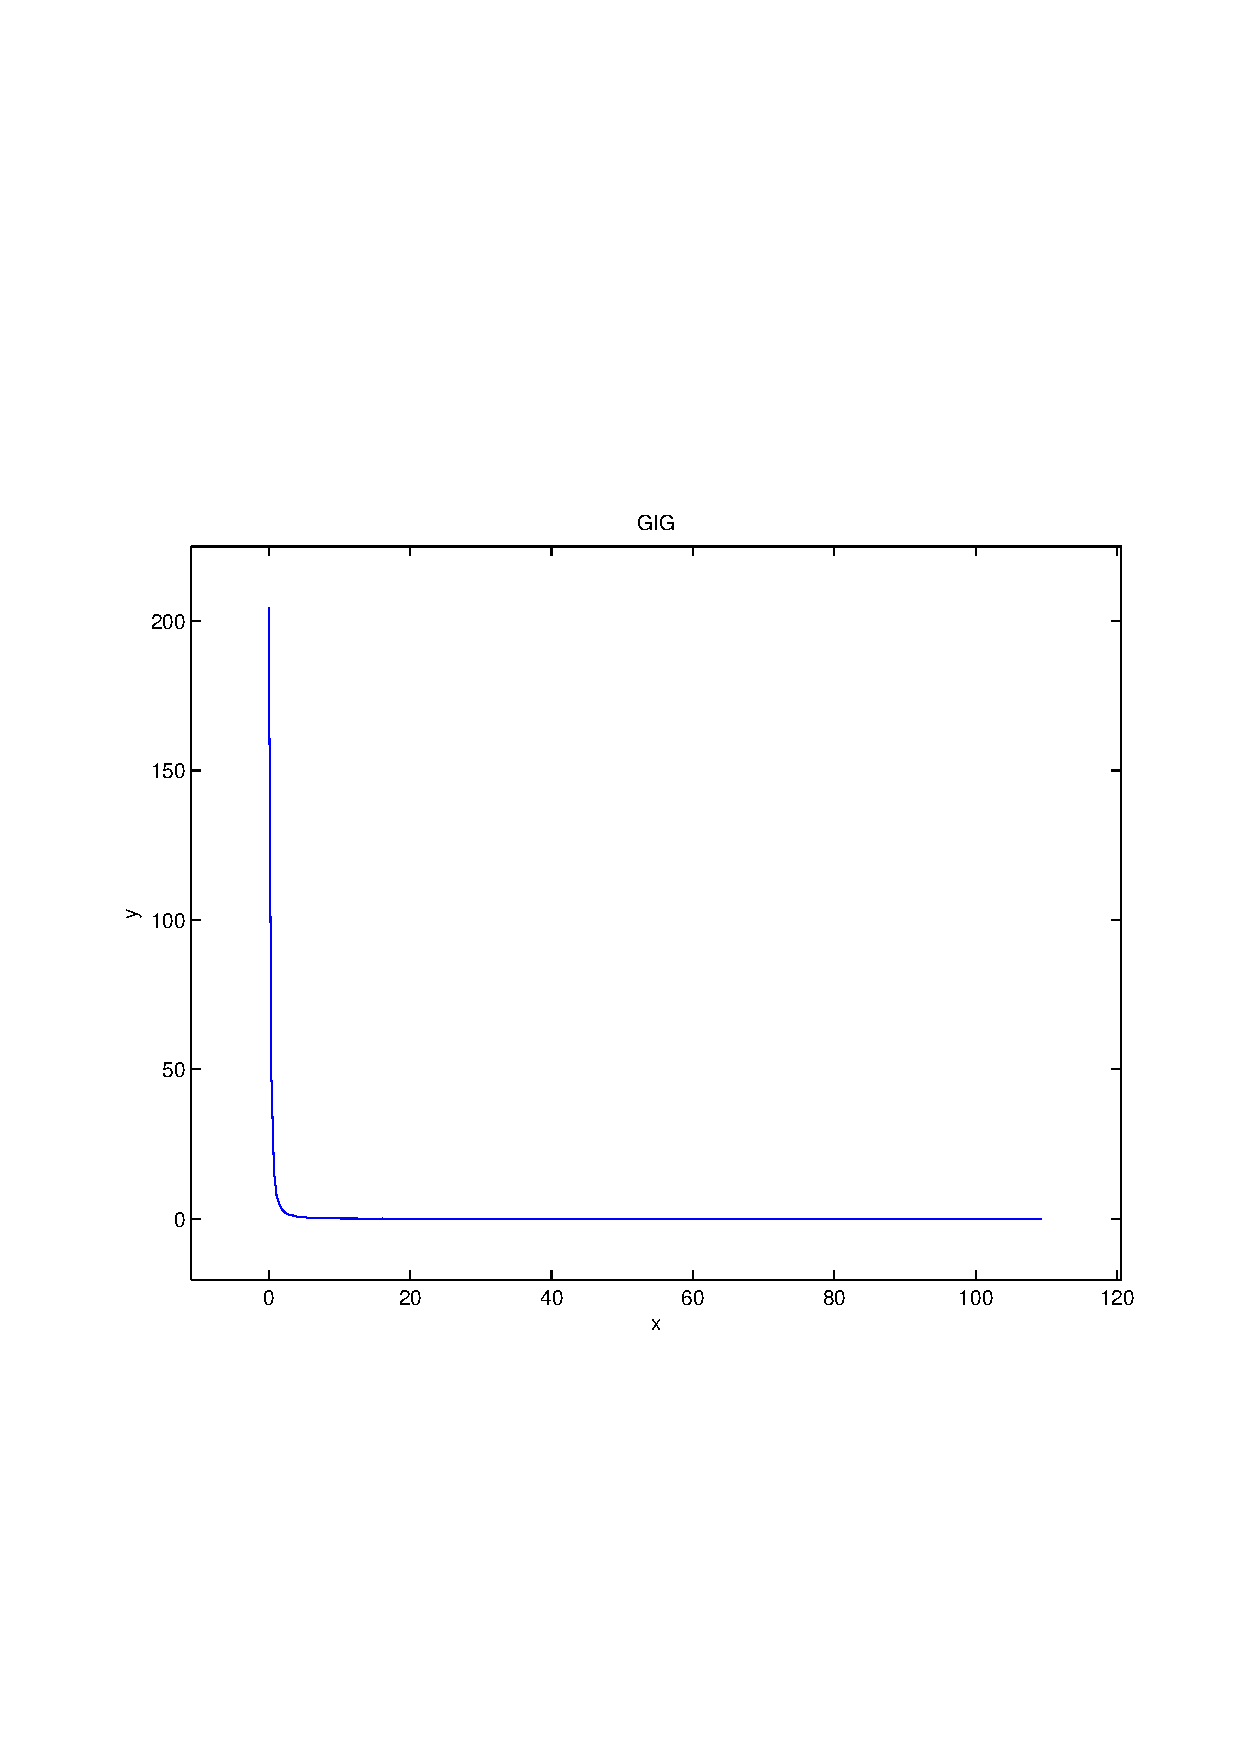
\includegraphics[width=5cm,height=5cm]{GIG.pdf}

normal-box-muller \begin{tabular}{|c|c|c|c|}  mean & variance & skewness & kurtosis \\  \hline
$\mu_1 = -0.00169$ & $\mu_2 = +1.00159$ & $\mu_3 = +0.00284$ & $\mu_4 =+2.98019$ \\
\end{tabular}

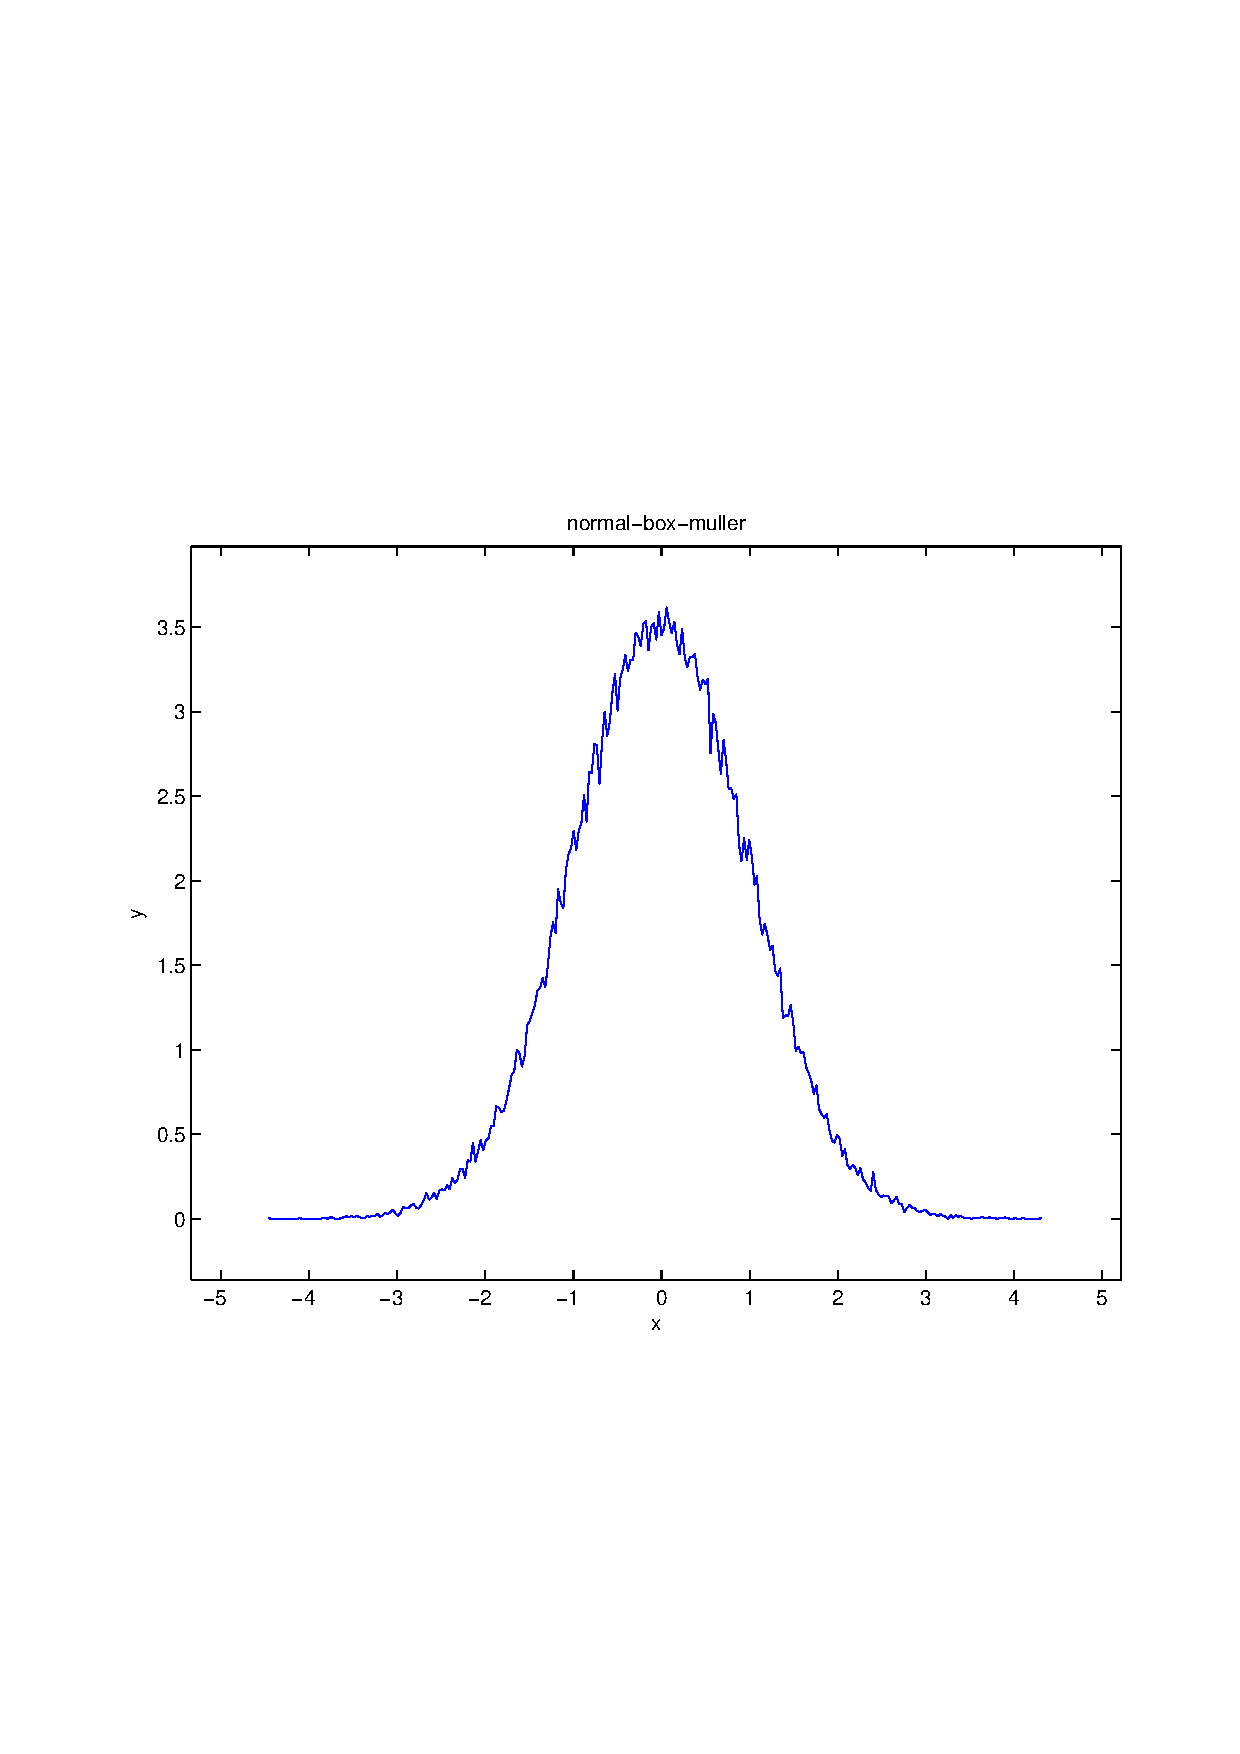
\includegraphics[width=5cm,height=5cm]{normal-box-muller.pdf}

\newpage
normal-inverse-approximation \begin{tabular}{|c|c|c|c|}  mean & variance & skewness & kurtosis \\  \hline
$\mu_1 = +0.00230$ & $\mu_2 = +1.00486$ & $\mu_3 = +0.01163$ & $\mu_4 =+2.99254$ \\
\end{tabular}

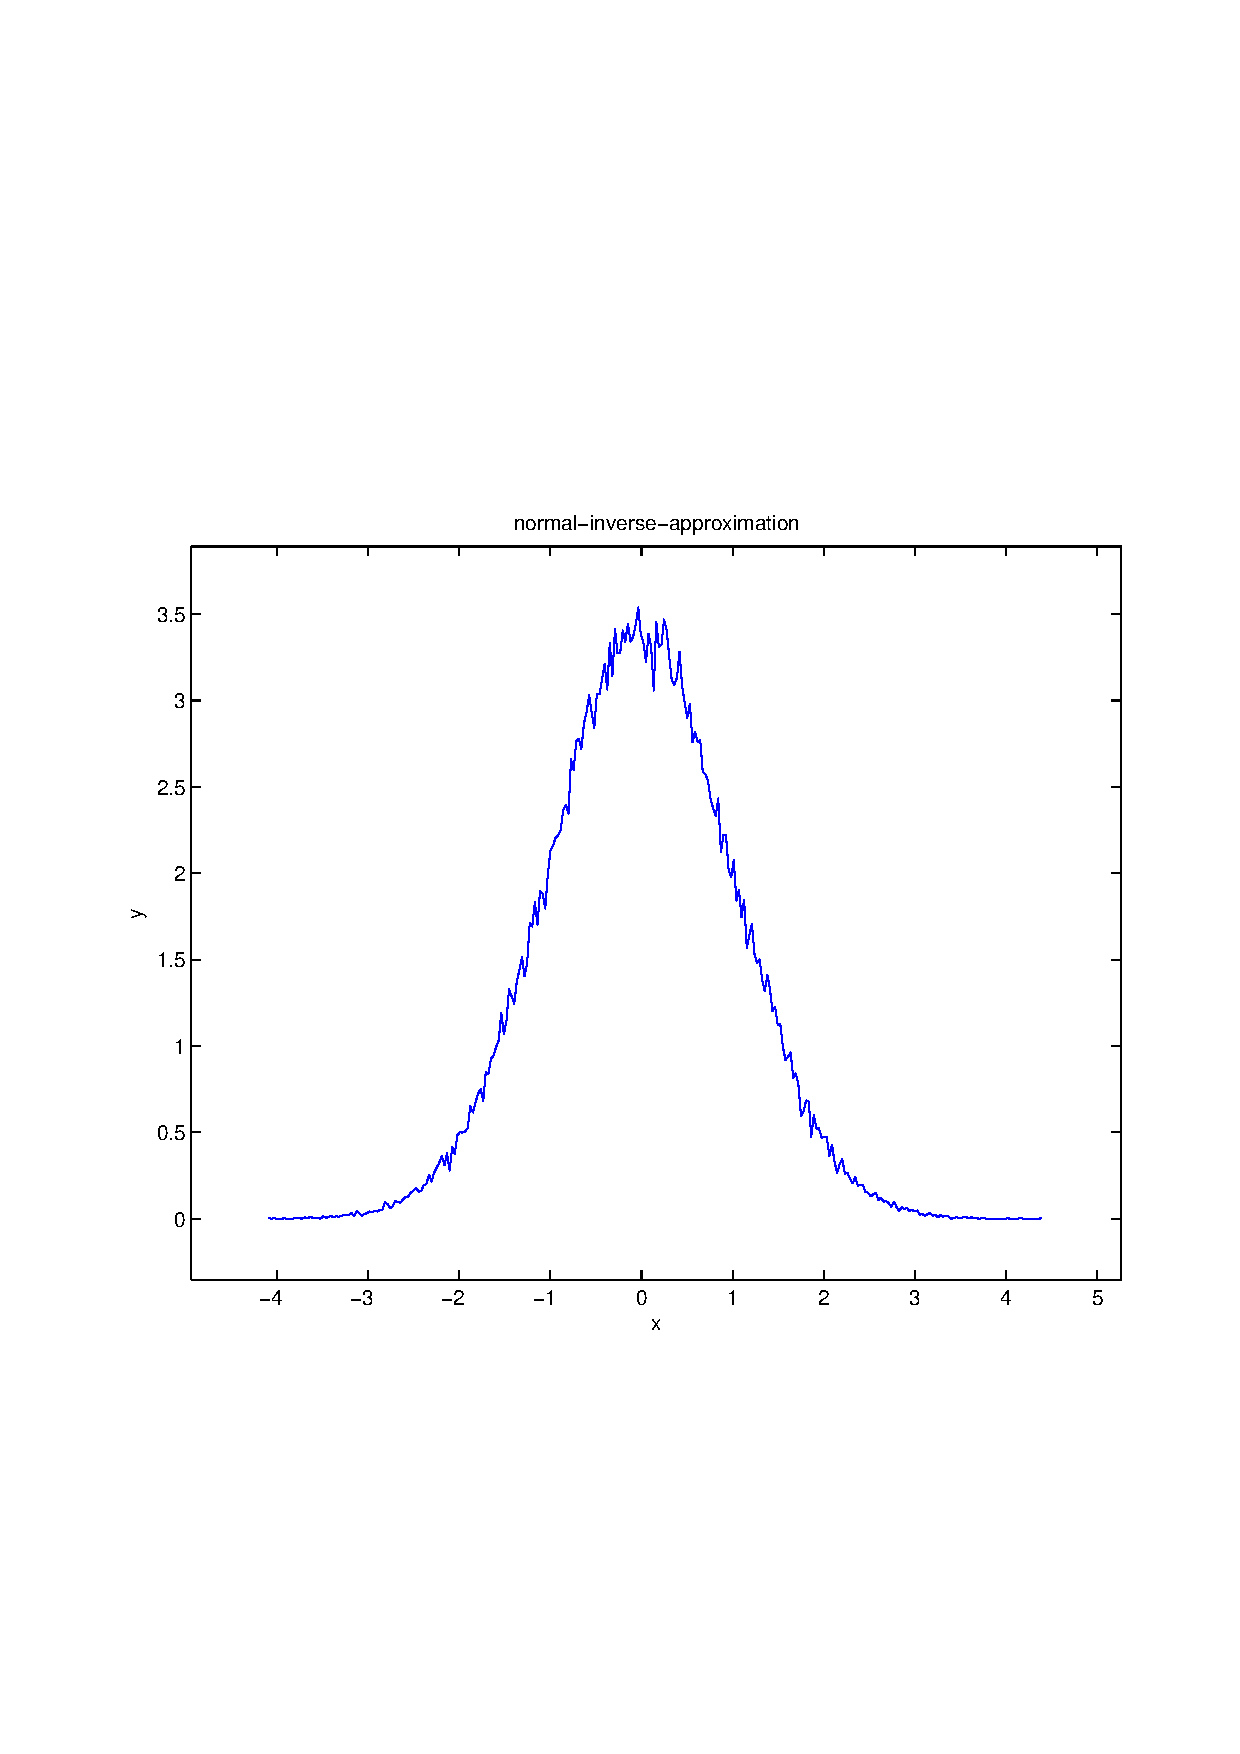
\includegraphics[width=5cm,height=5cm]{normal-inverse-approximation.pdf}

pareto \begin{tabular}{|c|c|c|c|}  mean & variance & skewness & kurtosis \\  \hline
$\mu_1 = +3184578.26493$ & $\mu_2 = +888468246174112900.00000$ & $\mu_3 = +315.36997$ & $\mu_4 =+99629.09819$ \\
\end{tabular}

\includegraphics[width=5cm,height=5cm]{pareto.pdf}

poisson \begin{tabular}{|c|c|c|c|}  mean & variance & skewness & kurtosis \\  \hline
$\mu_1 = +1.10595$ & $\mu_2 = +0.13160$ & $\mu_3 = +3.94092$ & $\mu_4 =+21.35260$ \\
\end{tabular}

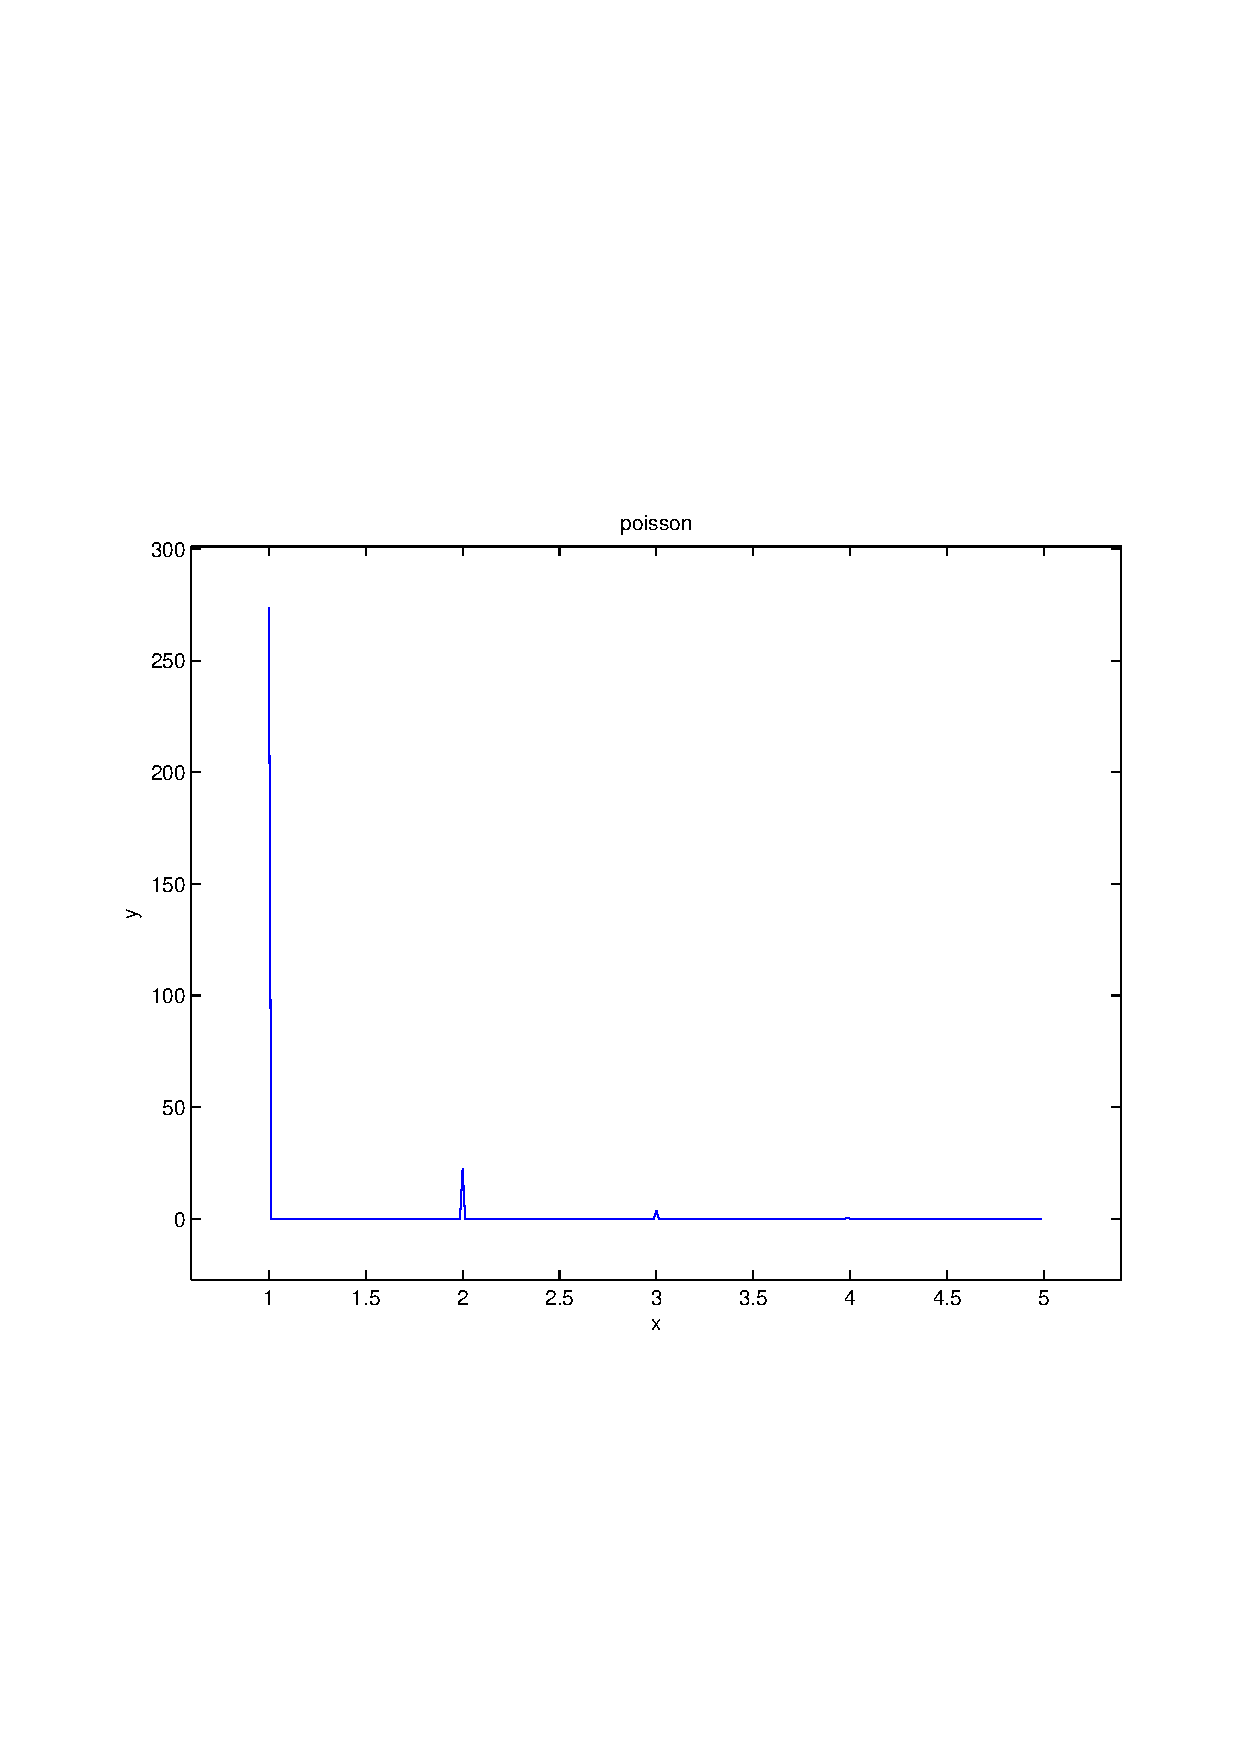
\includegraphics[width=5cm,height=5cm]{poisson.pdf}

\newpage
beta \begin{tabular}{|c|c|c|c|}  mean & variance & skewness & kurtosis \\  \hline
$\mu_1 = +0.33358$ & $\mu_2 = +0.12720$ & $\mu_3 = +0.68014$ & $\mu_4 =+1.90728$ \\
\end{tabular}

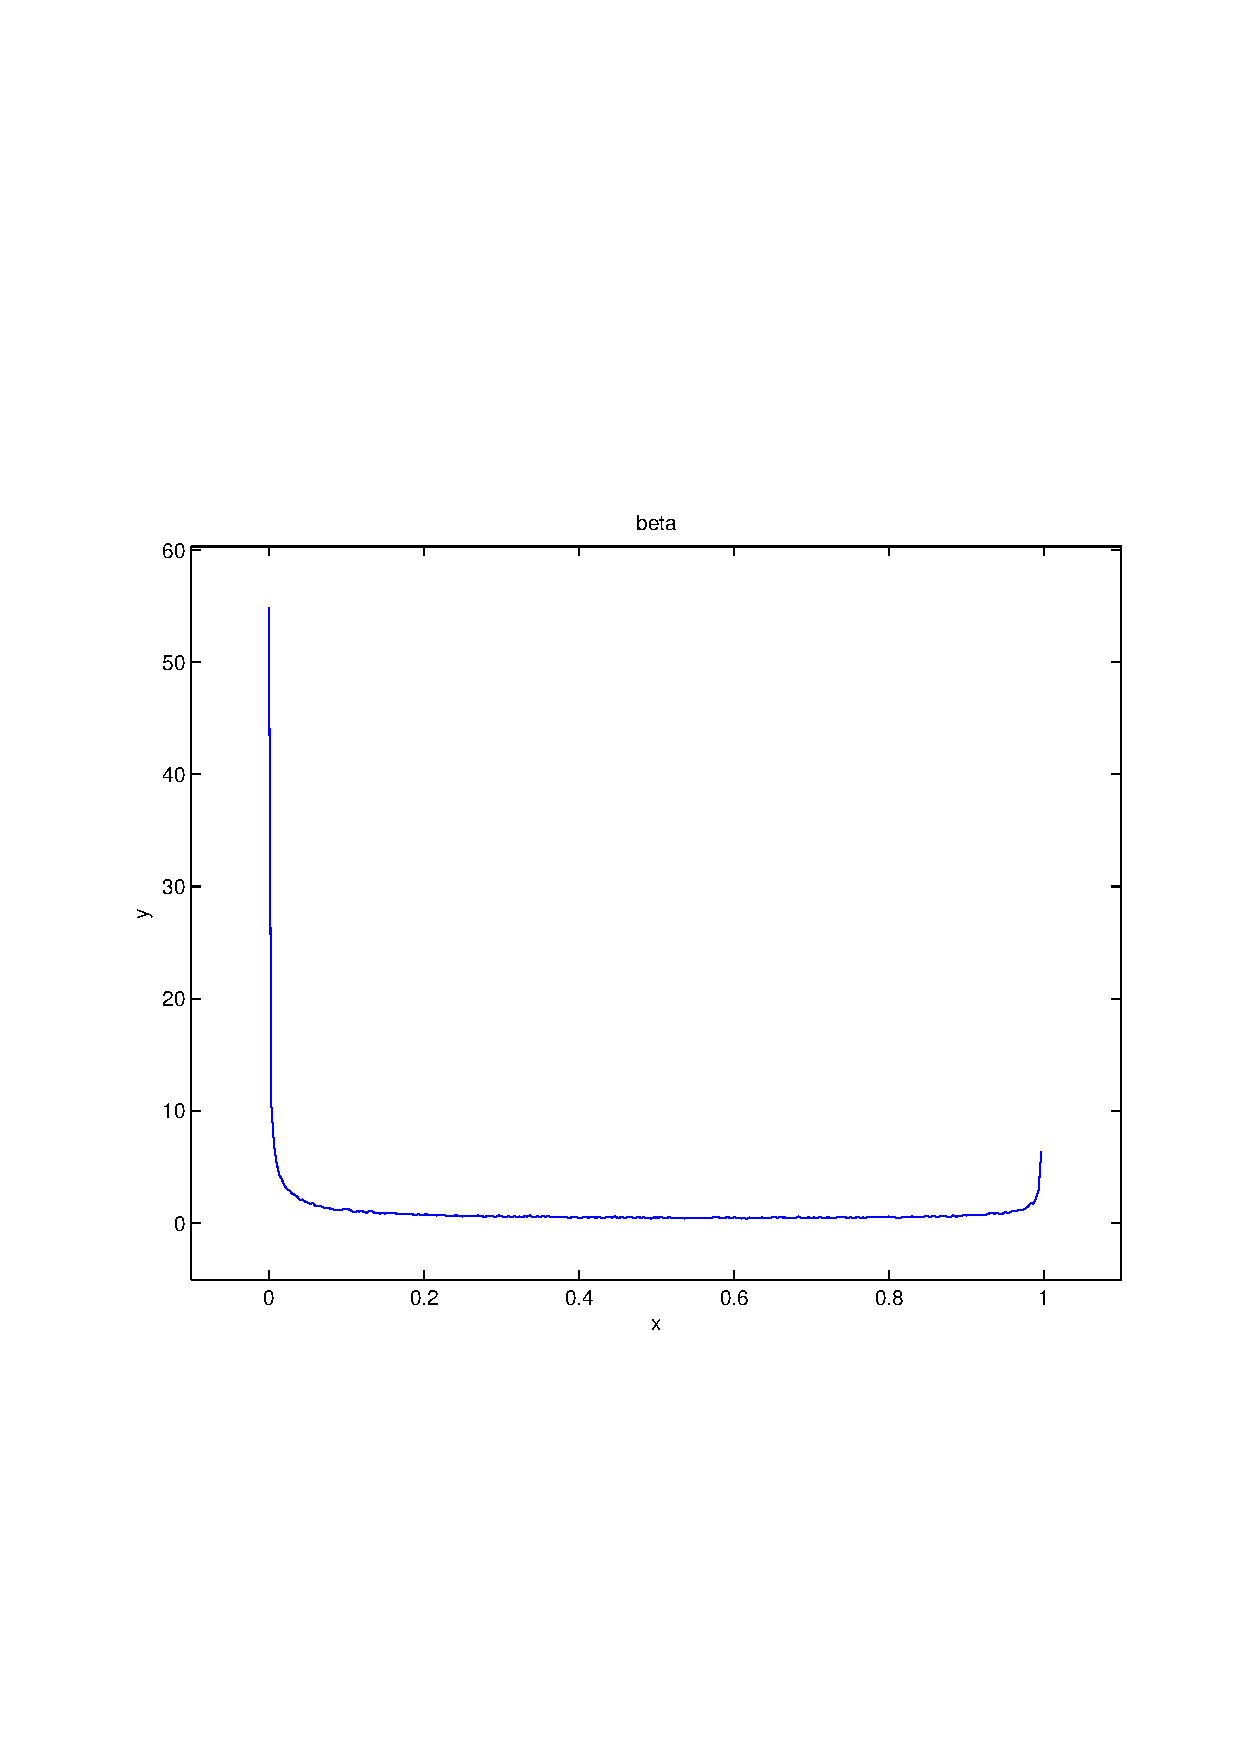
\includegraphics[width=5cm,height=5cm]{beta.pdf}

QueryPerformanceCounter  =  +16.94875
\subsubsection{Multiclass Support Vector Machine }
\begin{itemize}
\item Number or training points = 1024
\item Feature dimension = 3
\item Number or classes = 3
\end{itemize}
{The mean vectors of the 3 classes}

$\mu_1 = \left(
\begin{array}{
ccc}
+1.90000 & +0.10000 & +0.10000 \\
\end{array}
\right)$ \newline 

$\mu_2 = \left(
\begin{array}{
ccc}
+0.10000 & +1.90000 & +0.10000 \\
\end{array}
\right)$ \newline 

$\mu_3 = \left(
\begin{array}{
ccc}
+0.00000 & +0.00000 & +1.90000 \\
\end{array}
\right)$ \newline 

A random SPD covairance matrix is generated for each of the classes.\newline

$\rho_1 = \left(
\begin{array}{
ccc}
+3.484 & -0.077 & -0.245 \\
-0.077 & +2.854 & +0.065 \\
-0.245 & +0.065 & +2.804 \\
\end{array}
\right)$ \newline 

$\rho_2 = \left(
\begin{array}{
ccc}
+2.779 & -0.475 & -0.094 \\
-0.475 & +3.239 & +0.433 \\
-0.094 & +0.433 & +4.199 \\
\end{array}
\right)$ \newline 

$\rho_3 = \left(
\begin{array}{
ccc}
+1.828 & +0.200 & +0.300 \\
+0.200 & +2.617 & -0.102 \\
+0.300 & -0.102 & +1.891 \\
\end{array}
\right)$ \newline 

Verify $L_1$ condition number of covariance. The diagonal entries of the matrix have the form $(0.5 + U(0,1) )*dim(Dom(Cov))$
The lower-diagonal entries take the form $U(0,1) - 0.5$. 
The $L_1$ condition numbers are :
\begin{itemize}
\item +1.490
\item +2.011
\item +2.064
\end{itemize}
\includegraphics[width=10.0cm,height=10.0cm]{rv1_corr.pdf}

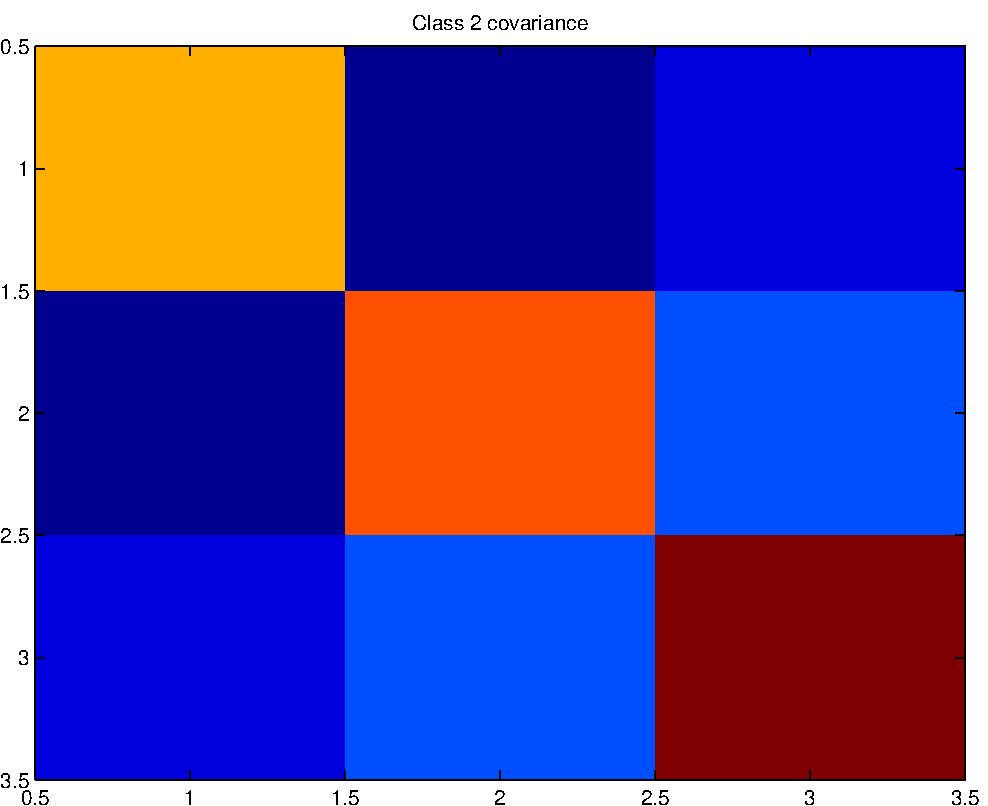
\includegraphics[width=10.0cm,height=10.0cm]{rv2_corr.pdf}

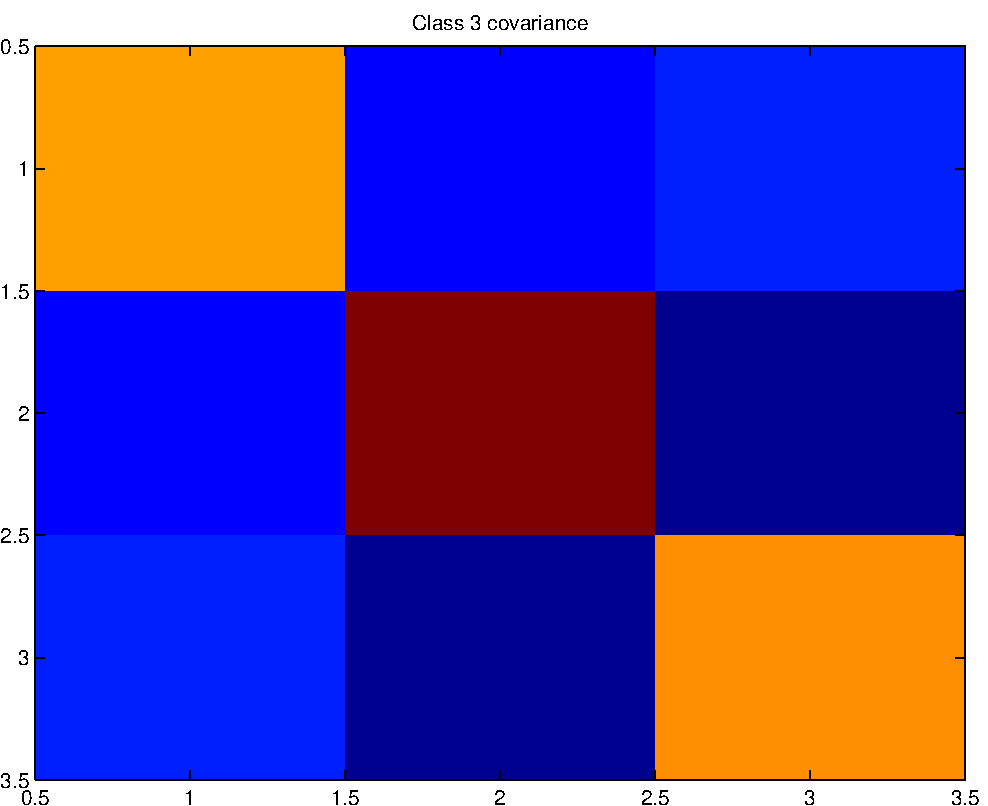
\includegraphics[width=10.0cm,height=10.0cm]{rv3_corr.pdf}

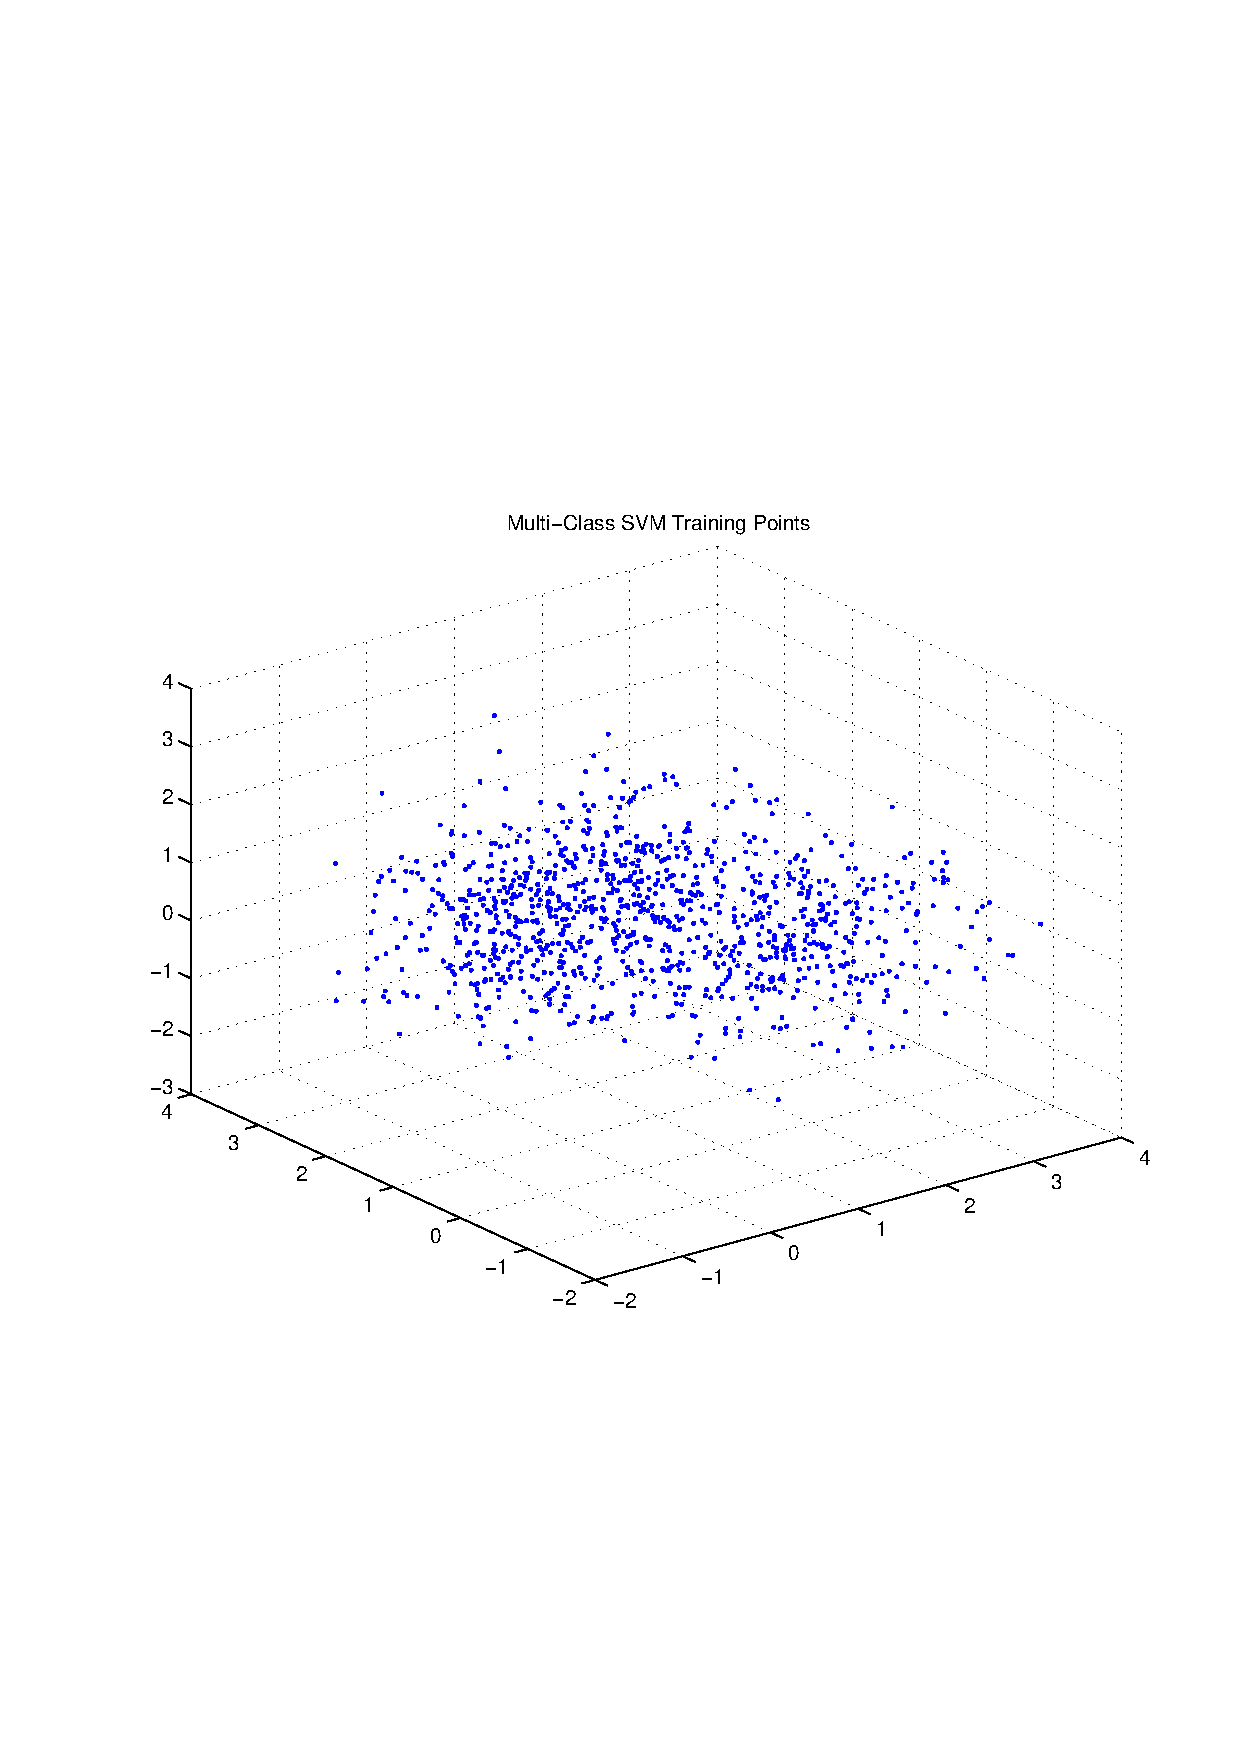
\includegraphics[width=10.0cm,height=10.0cm]{trainingPoints.pdf}

These are the SVM parameters - the RBF kernel is used\begin{itemize}
\item allOutlierFraction=0.05
\item mixingCoeff=0.3
\item smoThresh=1.0/10000.0
\item sigma=1
\end{itemize}
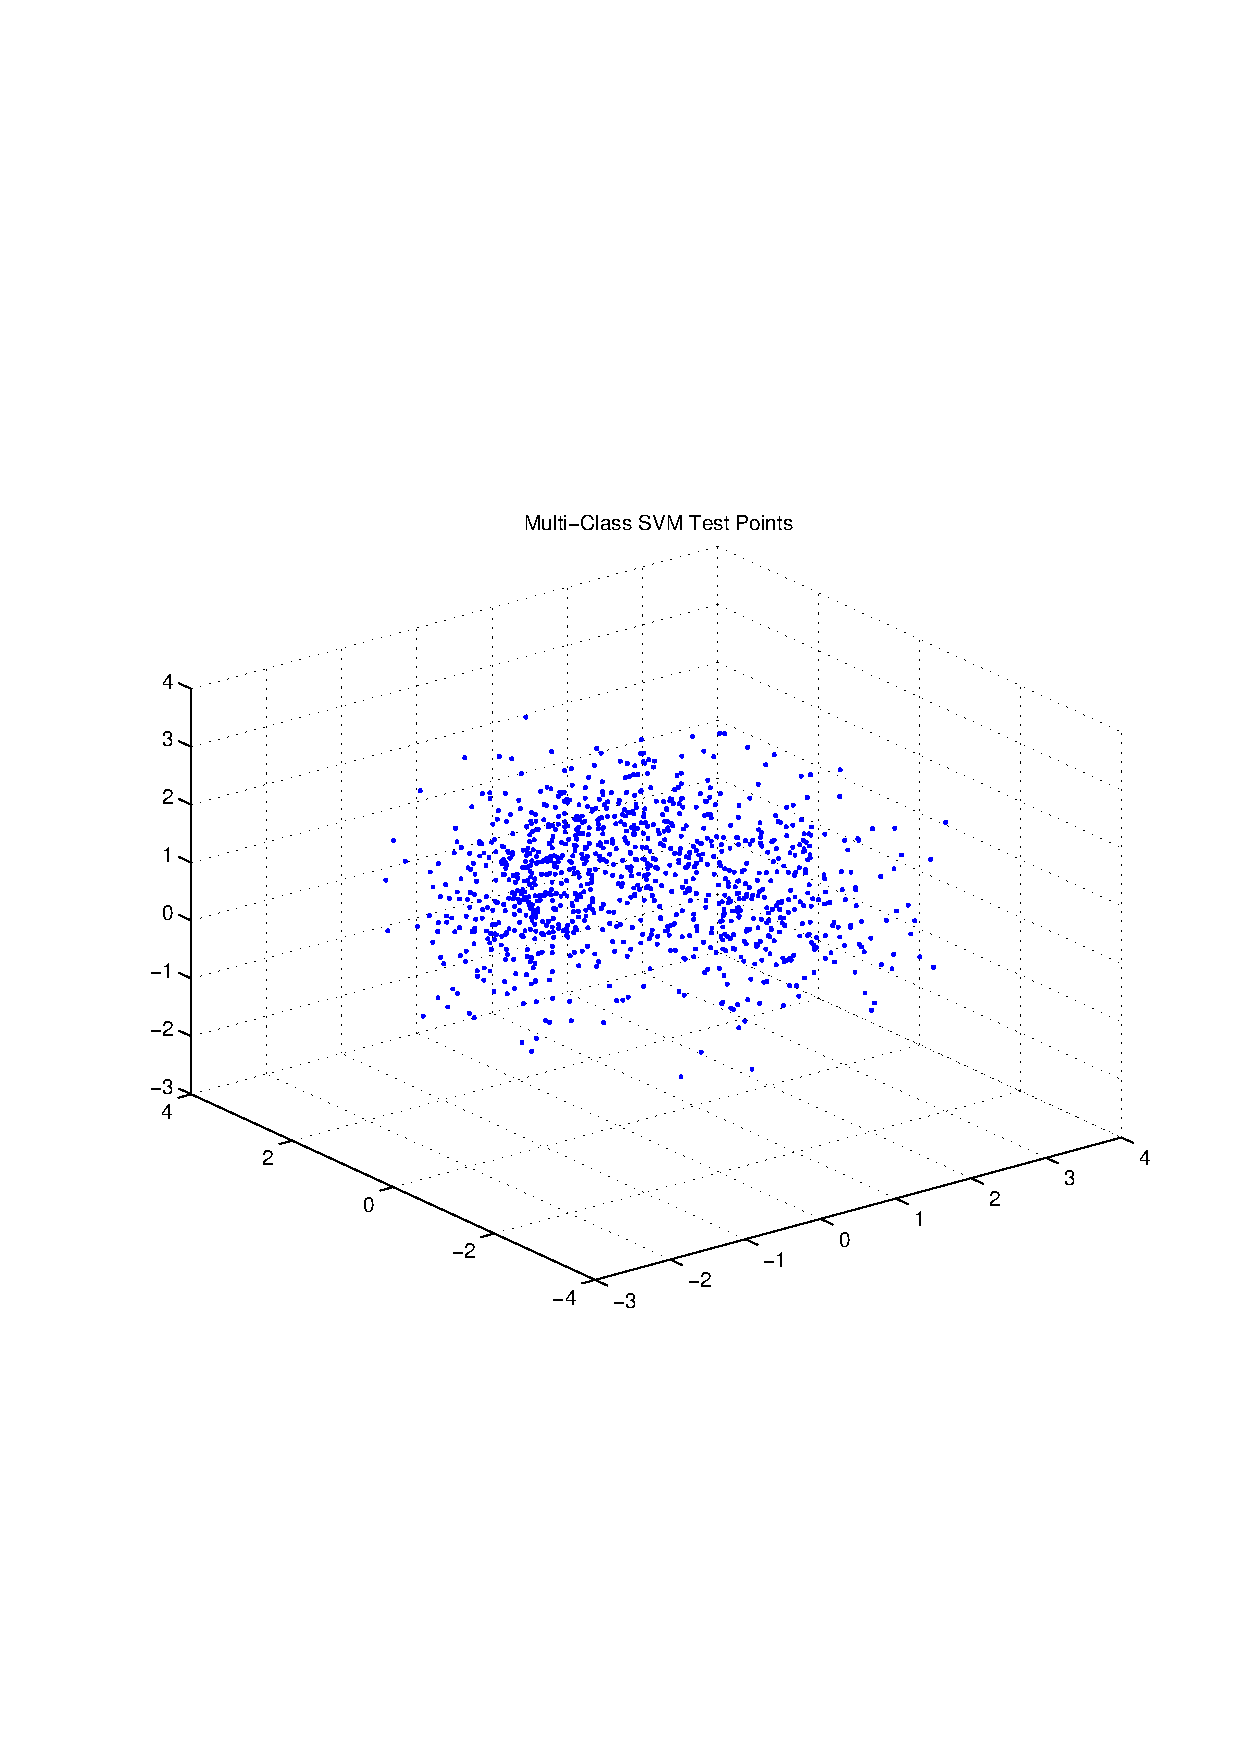
\includegraphics[width=10.0cm,height=10.0cm]{testPoints.pdf}

The marginal sample moments (mean var skew kurtosis) for training points.\newline
\begin{tabular}{ c |  c  c  c  c}
Feature & $\mu_1$ & $\mu_2$ & $\mu_3$ & $\mu_4$ \\
0 & +0.670 & +1.296 & +0.431& +2.469 \\
\hline
1 & +0.704 & +1.268 & +0.389& +2.408 \\
\hline
2 & +0.697 & +1.291 & +0.075& +2.268 \\
\hline
\end{tabular}
\newline
The marginal sample moments (mean var skew kurtosis) for test points.\newline
\begin{tabular}{ c | c  c  c  c}
Feature & $\mu_1$ & $\mu_2$ & $\mu_3$ & $\mu_4$ \\
0 & +0.678 & +1.216 & +0.587& +2.609\\
\hline
1 & +0.668 & +1.266 & +0.444& +2.436\\
\hline
2 & +0.721 & +1.245 & +0.044& +2.256\\
\hline
\end{tabular}\newline
\includegraphics[width=10.0cm,height=10.0cm]{classDiffs.pdf}

The error rate for this run is +0.071\newline
QueryPerformanceCounter  =  +4.962
\subsubsection{Semidefinite Programming SDPA}
QueryPerformanceCounter  =  +0.077
\subsubsection{Linear Regression 3x1}
\subsubsection{3 x 1 Linear Regression}
Sample size = 64

Number of features = 3

$\sigma = \left(
\begin{array}{
ccc}
+3.952 & -0.499 & -0.010 \\
-0.499 & +1.895 & +0.465 \\
-0.010 & +0.465 & +4.477 \\
\end{array}
\right)$ \newline 

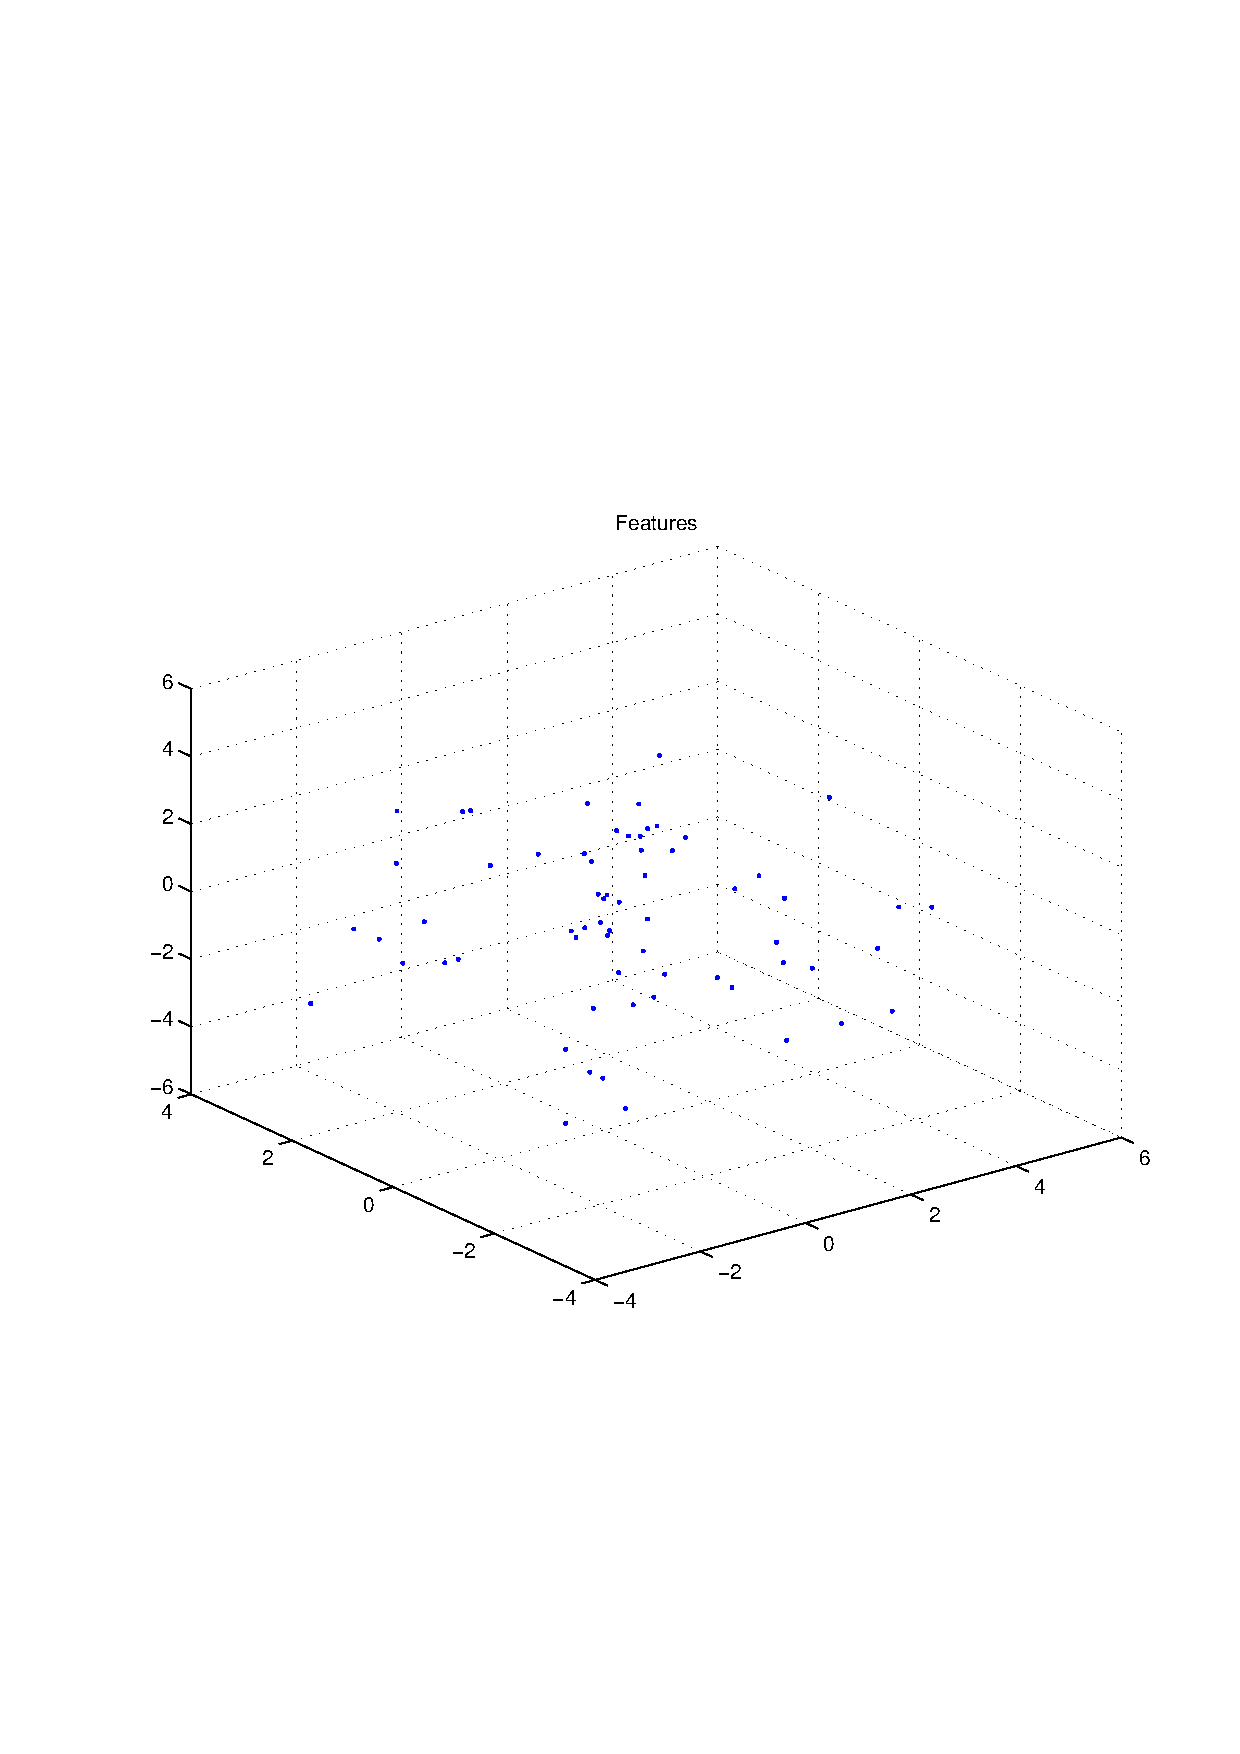
\includegraphics[width=10.0cm,height=10.0cm]{regression_features.pdf}

Beta
+0.817, +0.999, +0.510

Response
-0.381
+1.408
-1.713
+0.259
-1.306
+2.272
+1.266
+3.538
-0.637
+1.549
+0.578
+0.732
+1.308
+3.660
+2.464
+1.218
-1.373
+1.314
+0.704
+4.726
-0.599
+3.010
+0.758
+0.625
-3.797
+3.632
-0.636
-1.660
+1.251
+2.213
+4.689
+2.470
-2.245
+2.095
+2.124
+3.392
+3.957
+3.971
+2.550
+0.851
-5.725
-0.439
+3.625
+3.857
+4.110
-3.120
+2.110
+1.781
-1.776
-0.745
-3.564
+3.439
-3.030
-1.633
+0.022
-2.021
+4.097
-2.208
+0.514
-3.470
-0.888
-0.101
+0.895
+0.274
Estimate for Beta
-6277438562204192200000000000000000000000000000000000000000000000000.000
-6277438562204192200000000000000000000000000000000000000000000000000.000
-6277438562204192200000000000000000000000000000000000000000000000000.000
Error:
+0.000, +0.000, +0.000


QueryPerformanceCounter  =  +0.721
\subsubsection{Matrix Norms}
\subsubsection{Haar Distributed Random Orthogonal Matrix $A \in O(n)$}
 Testing Operator Norm
Number of Dimensions: +12

$A = \left(
\begin{array}{
cccccccccccc}
+0.036 & -0.263 & +0.538 & +0.353 & -0.100 & -0.152 & -0.256 & -0.313 & +0.128 & +0.052 & -0.185 & +0.516 \\
+0.116 & +0.111 & -0.028 & +0.205 & +0.323 & +0.460 & -0.187 & -0.037 & +0.530 & -0.216 & -0.437 & -0.246 \\
-0.547 & -0.032 & -0.027 & +0.383 & -0.062 & +0.144 & -0.217 & -0.150 & -0.306 & +0.440 & -0.127 & -0.394 \\
+0.219 & +0.062 & -0.297 & -0.273 & +0.166 & -0.209 & -0.469 & -0.257 & -0.461 & -0.124 & -0.443 & +0.063 \\
-0.269 & -0.556 & +0.105 & -0.138 & -0.166 & +0.018 & -0.018 & -0.167 & -0.066 & -0.653 & +0.056 & -0.314 \\
+0.018 & -0.335 & +0.079 & +0.203 & +0.525 & -0.329 & -0.230 & +0.623 & -0.061 & +0.005 & +0.069 & -0.086 \\
+0.055 & -0.111 & +0.062 & +0.184 & +0.402 & -0.073 & +0.741 & -0.224 & -0.273 & -0.020 & -0.324 & -0.010 \\
+0.292 & -0.460 & -0.224 & -0.160 & +0.005 & -0.266 & +0.015 & -0.327 & +0.386 & +0.454 & +0.057 & -0.301 \\
+0.417 & -0.027 & +0.549 & -0.204 & -0.301 & +0.154 & +0.026 & +0.270 & -0.228 & +0.172 & -0.273 & -0.371 \\
+0.447 & +0.035 & +0.081 & +0.289 & +0.230 & +0.285 & -0.150 & -0.309 & -0.289 & -0.084 & +0.589 & -0.138 \\
+0.005 & +0.498 & +0.203 & +0.202 & -0.057 & -0.638 & -0.010 & -0.159 & +0.157 & -0.219 & +0.036 & -0.400 \\
-0.321 & +0.139 & +0.448 & -0.571 & +0.493 & +0.061 & -0.079 & -0.213 & +0.073 & +0.154 & +0.154 & -0.016 \\
\end{array}
\right)$ \newline 

$Det(A) :   A \in O(n)$ = (-1.000,+0.000)

$L = \left(
\begin{array}{
cccccccccccc}
+1.000 & +0.000 & +0.000 & +0.000 & +0.000 & +0.000 & +0.000 & +0.000 & +0.000 & +0.000 & +0.000 & +0.000 \\
+0.491 & +1.000 & +0.000 & +0.000 & +0.000 & +0.000 & +0.000 & +0.000 & +0.000 & +0.000 & +0.000 & +0.000 \\
-0.764 & +0.095 & +1.000 & +0.000 & +0.000 & +0.000 & +0.000 & +0.000 & +0.000 & +0.000 & +0.000 & +0.000 \\
+0.588 & -0.292 & +0.964 & +1.000 & +0.000 & +0.000 & +0.000 & +0.000 & +0.000 & +0.000 & +0.000 & +0.000 \\
-0.033 & +0.622 & +0.009 & -0.415 & +1.000 & +0.000 & +0.000 & +0.000 & +0.000 & +0.000 & +0.000 & +0.000 \\
-0.010 & -0.922 & +0.603 & +0.167 & -0.123 & +1.000 & +0.000 & +0.000 & +0.000 & +0.000 & +0.000 & +0.000 \\
-0.100 & +0.212 & +0.066 & -0.282 & +0.714 & -0.176 & +1.000 & +0.000 & +0.000 & +0.000 & +0.000 & +0.000 \\
-0.818 & -0.017 & +0.117 & -0.579 & +0.726 & -0.589 & +0.023 & +1.000 & +0.000 & +0.000 & +0.000 & +0.000 \\
-0.400 & -0.091 & -0.573 & +0.080 & -0.135 & +0.041 & -0.730 & +0.584 & +1.000 & +0.000 & +0.000 & +0.000 \\
-0.535 & +0.883 & -0.663 & -0.410 & +0.213 & -0.003 & -0.155 & +0.503 & -0.046 & +1.000 & +0.000 & +0.000 \\
-0.213 & -0.192 & -0.021 & -0.225 & +0.485 & -0.733 & -0.001 & +0.511 & -0.797 & -0.097 & +1.000 & +0.000 \\
-0.066 & +0.492 & +0.923 & -0.426 & +0.653 & +0.257 & +0.024 & +0.735 & -0.529 & +0.538 & +0.478 & +1.000 \\
\end{array}
\right)$ \newline 

$U = \left(
\begin{array}{
cccccccccccc}
-0.547 & -0.032 & -0.027 & +0.383 & -0.062 & +0.144 & -0.217 & -0.150 & -0.306 & +0.440 & -0.127 & -0.394 \\
+0.000 & -0.540 & +0.119 & -0.327 & -0.136 & -0.052 & +0.089 & -0.093 & +0.085 & -0.870 & +0.118 & -0.120 \\
+0.000 & +0.000 & +0.517 & +0.120 & -0.335 & +0.269 & -0.148 & +0.165 & -0.469 & +0.590 & -0.381 & -0.660 \\
+0.000 & +0.000 & +0.000 & -1.007 & +0.812 & -0.298 & +0.217 & -0.310 & +0.730 & -0.927 & +0.630 & +0.817 \\
+0.000 & +0.000 & +0.000 & +0.000 & +0.947 & -0.418 & -0.201 & +0.545 & +0.183 & +0.170 & +0.256 & +0.321 \\
+0.000 & +0.000 & +0.000 & +0.000 & +0.000 & -0.849 & +0.098 & -0.227 & +0.416 & -1.197 & +0.300 & -0.213 \\
+0.000 & +0.000 & +0.000 & +0.000 & +0.000 & +0.000 & +0.933 & -0.747 & -0.143 & -0.423 & -0.289 & -0.017 \\
+0.000 & +0.000 & +0.000 & +0.000 & +0.000 & +0.000 & +0.000 & -1.145 & +0.055 & -1.164 & +0.894 & -0.271 \\
+0.000 & +0.000 & +0.000 & +0.000 & +0.000 & +0.000 & +0.000 & +0.000 & -1.032 & +0.827 & -1.463 & -0.352 \\
+0.000 & +0.000 & +0.000 & +0.000 & +0.000 & +0.000 & +0.000 & +0.000 & +0.000 & +1.988 & -0.726 & -0.460 \\
+0.000 & +0.000 & +0.000 & +0.000 & +0.000 & +0.000 & +0.000 & +0.000 & +0.000 & +0.000 & -1.905 & -0.683 \\
+0.000 & +0.000 & +0.000 & +0.000 & +0.000 & +0.000 & +0.000 & +0.000 & +0.000 & +0.000 & +0.000 & +1.938 \\
\end{array}
\right)$ \newline 

$L * U  = \left(
\begin{array}{
cccccccccccc}
-0.547 & -0.032 & -0.027 & +0.383 & -0.062 & +0.144 & -0.217 & -0.150 & -0.306 & +0.440 & -0.127 & -0.394 \\
-0.269 & -0.556 & +0.105 & -0.138 & -0.166 & +0.018 & -0.018 & -0.167 & -0.066 & -0.653 & +0.056 & -0.314 \\
+0.417 & -0.027 & +0.549 & -0.204 & -0.301 & +0.154 & +0.026 & +0.270 & -0.228 & +0.172 & -0.273 & -0.371 \\
-0.321 & +0.139 & +0.448 & -0.571 & +0.493 & +0.061 & -0.079 & -0.213 & +0.073 & +0.154 & +0.154 & -0.016 \\
+0.018 & -0.335 & +0.079 & +0.203 & +0.525 & -0.329 & -0.230 & +0.623 & -0.061 & +0.005 & +0.069 & -0.086 \\
+0.005 & +0.498 & +0.203 & +0.202 & -0.057 & -0.638 & -0.010 & -0.159 & +0.157 & -0.219 & +0.036 & -0.400 \\
+0.055 & -0.111 & +0.062 & +0.184 & +0.402 & -0.073 & +0.741 & -0.224 & -0.273 & -0.020 & -0.324 & -0.010 \\
+0.447 & +0.035 & +0.081 & +0.289 & +0.230 & +0.285 & -0.150 & -0.309 & -0.289 & -0.084 & +0.589 & -0.138 \\
+0.219 & +0.062 & -0.297 & -0.273 & +0.166 & -0.209 & -0.469 & -0.257 & -0.461 & -0.124 & -0.443 & +0.063 \\
+0.292 & -0.460 & -0.224 & -0.160 & +0.005 & -0.266 & +0.015 & -0.327 & +0.386 & +0.454 & +0.057 & -0.301 \\
+0.116 & +0.111 & -0.028 & +0.205 & +0.323 & +0.460 & -0.187 & -0.037 & +0.530 & -0.216 & -0.437 & -0.246 \\
+0.036 & -0.263 & +0.538 & +0.353 & -0.100 & -0.152 & -0.256 & -0.313 & +0.128 & +0.052 & -0.185 & +0.516 \\
\end{array}
\right)$ \newline 

$Det(L) :    = (+1.000,+0.000)     Det(U) :    = (-1.000,+0.000)     Det(LU) :    = (-1.000,-0.000)$

$||A||_{L_1}$  = +3.166

$||A||_{L_{\infty}}$ = +3.043

$||A^{-1}||_{L_1}$  = +3.043

$||A^{-1}||_{L_{\infty}}$ = +3.166

$||A||_{L_{\infty}} * ||A^{-1}||_{L_{\infty}} = +9.634$

$||A||_{L_1} * ||A^{-1}||_{L_1} = +9.634$

Frobenious Norm  $||A||_{\textit{F}}$ via $\sum\limits_{i,j =0}^{n} \|A_{i,j}|$   of  $A \in O(n)$  +3.464

$L_1$ condition number of Haar Distributed Random Orthogonal Matrix $A \in O(n)$ +9.634

$A = \left(
\begin{array}{
cccccccccccc}
+0.036 & -0.263 & +0.538 & +0.353 & -0.100 & -0.152 & -0.256 & -0.313 & +0.128 & +0.052 & -0.185 & +0.516 \\
+0.116 & +0.111 & -0.028 & +0.205 & +0.323 & +0.460 & -0.187 & -0.037 & +0.530 & -0.216 & -0.437 & -0.246 \\
-0.547 & -0.032 & -0.027 & +0.383 & -0.062 & +0.144 & -0.217 & -0.150 & -0.306 & +0.440 & -0.127 & -0.394 \\
+0.219 & +0.062 & -0.297 & -0.273 & +0.166 & -0.209 & -0.469 & -0.257 & -0.461 & -0.124 & -0.443 & +0.063 \\
-0.269 & -0.556 & +0.105 & -0.138 & -0.166 & +0.018 & -0.018 & -0.167 & -0.066 & -0.653 & +0.056 & -0.314 \\
+0.018 & -0.335 & +0.079 & +0.203 & +0.525 & -0.329 & -0.230 & +0.623 & -0.061 & +0.005 & +0.069 & -0.086 \\
+0.055 & -0.111 & +0.062 & +0.184 & +0.402 & -0.073 & +0.741 & -0.224 & -0.273 & -0.020 & -0.324 & -0.010 \\
+0.292 & -0.460 & -0.224 & -0.160 & +0.005 & -0.266 & +0.015 & -0.327 & +0.386 & +0.454 & +0.057 & -0.301 \\
+0.417 & -0.027 & +0.549 & -0.204 & -0.301 & +0.154 & +0.026 & +0.270 & -0.228 & +0.172 & -0.273 & -0.371 \\
+0.447 & +0.035 & +0.081 & +0.289 & +0.230 & +0.285 & -0.150 & -0.309 & -0.289 & -0.084 & +0.589 & -0.138 \\
+0.005 & +0.498 & +0.203 & +0.202 & -0.057 & -0.638 & -0.010 & -0.159 & +0.157 & -0.219 & +0.036 & -0.400 \\
-0.321 & +0.139 & +0.448 & -0.571 & +0.493 & +0.061 & -0.079 & -0.213 & +0.073 & +0.154 & +0.154 & -0.016 \\
\end{array}
\right)$ \newline 

$L_{\infty}$ condition number of Haar Distributed Random Orthogonal Matrix $A \in O(n)$ +8.035

Eigenvalues of $A \in O(n)$

(-1.000,+0.000), (-0.835,+0.550), (-0.835,-0.550), (-0.269,+0.963), (-0.269,-0.963), (+0.410,+0.912), (+0.410,-0.912), (+0.136,+0.991), (+0.136,-0.991), (+0.295,+0.956), (+0.295,-0.956), (+1.000,+0.000)

 $|\lambda | : \lambda \in \sigma(A) , A \in O(n)$

+1.000, +1.000, +1.000, +1.000, +1.000, +1.000, +1.000, +1.000, +1.000, +1.000, +1.000, +1.000


Calculating $A^{\dag} A,$  we expect $A^{\dag} A \approx I$

$A^{\dag} A = \left(
\begin{array}{
cccccccccccc}
+1.000 & +0.000 & -0.000 & +0.000 & +0.000 & -0.000 & -0.000 & +0.000 & +0.000 & +0.000 & -0.000 & +0.000 \\
+0.000 & +1.000 & -0.000 & +0.000 & +0.000 & +0.000 & +0.000 & +0.000 & +0.000 & -0.000 & -0.000 & +0.000 \\
-0.000 & -0.000 & +1.000 & +0.000 & -0.000 & +0.000 & +0.000 & +0.000 & -0.000 & +0.000 & -0.000 & +0.000 \\
+0.000 & +0.000 & +0.000 & +1.000 & +0.000 & -0.000 & -0.000 & -0.000 & -0.000 & +0.000 & -0.000 & -0.000 \\
+0.000 & +0.000 & -0.000 & +0.000 & +1.000 & -0.000 & +0.000 & +0.000 & +0.000 & +0.000 & +0.000 & +0.000 \\
-0.000 & +0.000 & +0.000 & -0.000 & -0.000 & +1.000 & -0.000 & +0.000 & -0.000 & -0.000 & -0.000 & -0.000 \\
-0.000 & +0.000 & +0.000 & -0.000 & +0.000 & -0.000 & +1.000 & -0.000 & -0.000 & -0.000 & -0.000 & -0.000 \\
+0.000 & +0.000 & +0.000 & -0.000 & +0.000 & +0.000 & -0.000 & +1.000 & -0.000 & +0.000 & -0.000 & -0.000 \\
+0.000 & +0.000 & -0.000 & -0.000 & +0.000 & -0.000 & -0.000 & -0.000 & +1.000 & +0.000 & +0.000 & +0.000 \\
+0.000 & -0.000 & +0.000 & +0.000 & +0.000 & -0.000 & -0.000 & +0.000 & +0.000 & +1.000 & +0.000 & +0.000 \\
-0.000 & -0.000 & -0.000 & -0.000 & +0.000 & -0.000 & -0.000 & -0.000 & +0.000 & +0.000 & +1.000 & -0.000 \\
+0.000 & +0.000 & +0.000 & -0.000 & +0.000 & -0.000 & -0.000 & -0.000 & +0.000 & +0.000 & -0.000 & +1.000 \\
\end{array}
\right)$ \newline 

Calculating $A^{-1} ,  A \in O(n)$.

$A^{-1} = \left(
\begin{array}{
cccccccccccc}
+0.036 & +0.116 & -0.547 & +0.219 & -0.269 & +0.018 & +0.055 & +0.292 & +0.417 & +0.447 & +0.005 & -0.321 \\
-0.263 & +0.111 & -0.032 & +0.062 & -0.556 & -0.335 & -0.111 & -0.460 & -0.027 & +0.035 & +0.498 & +0.139 \\
+0.538 & -0.028 & -0.027 & -0.297 & +0.105 & +0.079 & +0.062 & -0.224 & +0.549 & +0.081 & +0.203 & +0.448 \\
+0.353 & +0.205 & +0.383 & -0.273 & -0.138 & +0.203 & +0.184 & -0.160 & -0.204 & +0.289 & +0.202 & -0.571 \\
-0.100 & +0.323 & -0.062 & +0.166 & -0.166 & +0.525 & +0.402 & +0.005 & -0.301 & +0.230 & -0.057 & +0.493 \\
-0.152 & +0.460 & +0.144 & -0.209 & +0.018 & -0.329 & -0.073 & -0.266 & +0.154 & +0.285 & -0.638 & +0.061 \\
-0.256 & -0.187 & -0.217 & -0.469 & -0.018 & -0.230 & +0.741 & +0.015 & +0.026 & -0.150 & -0.010 & -0.079 \\
-0.313 & -0.037 & -0.150 & -0.257 & -0.167 & +0.623 & -0.224 & -0.327 & +0.270 & -0.309 & -0.159 & -0.213 \\
+0.128 & +0.530 & -0.306 & -0.461 & -0.066 & -0.061 & -0.273 & +0.386 & -0.228 & -0.289 & +0.157 & +0.073 \\
+0.052 & -0.216 & +0.440 & -0.124 & -0.653 & +0.005 & -0.020 & +0.454 & +0.172 & -0.084 & -0.219 & +0.154 \\
-0.185 & -0.437 & -0.127 & -0.443 & +0.056 & +0.069 & -0.324 & +0.057 & -0.273 & +0.589 & +0.036 & +0.154 \\
+0.516 & -0.246 & -0.394 & +0.063 & -0.314 & -0.086 & -0.010 & -0.301 & -0.371 & -0.138 & -0.400 & -0.016 \\
\end{array}
\right)$ \newline 

Calculating $A^{-1} *A  ,  A \in O(n)$.   We expect $A^{-1} *A  \approx I$. 

$A^{-1} *A = \left(
\begin{array}{
cccccccccccc}
+1.000 & -0.000 & +0.000 & -0.000 & +0.000 & -0.000 & +0.000 & -0.000 & +0.000 & -0.000 & -0.000 & +0.000 \\
-0.000 & +1.000 & -0.000 & +0.000 & -0.000 & -0.000 & -0.000 & +0.000 & -0.000 & +0.000 & -0.000 & +0.000 \\
-0.000 & +0.000 & +1.000 & +0.000 & +0.000 & -0.000 & +0.000 & -0.000 & +0.000 & -0.000 & +0.000 & +0.000 \\
+0.000 & +0.000 & +0.000 & +1.000 & +0.000 & -0.000 & -0.000 & -0.000 & +0.000 & -0.000 & +0.000 & +0.000 \\
+0.000 & +0.000 & -0.000 & +0.000 & +1.000 & +0.000 & +0.000 & -0.000 & +0.000 & -0.000 & +0.000 & -0.000 \\
-0.000 & +0.000 & +0.000 & +0.000 & +0.000 & +1.000 & +0.000 & -0.000 & -0.000 & +0.000 & -0.000 & +0.000 \\
+0.000 & +0.000 & +0.000 & +0.000 & +0.000 & -0.000 & +1.000 & +0.000 & -0.000 & -0.000 & +0.000 & -0.000 \\
+0.000 & -0.000 & +0.000 & -0.000 & +0.000 & -0.000 & -0.000 & +1.000 & -0.000 & +0.000 & +0.000 & -0.000 \\
-0.000 & -0.000 & +0.000 & +0.000 & -0.000 & -0.000 & +0.000 & -0.000 & +1.000 & -0.000 & -0.000 & +0.000 \\
-0.000 & +0.000 & +0.000 & -0.000 & +0.000 & +0.000 & -0.000 & +0.000 & +0.000 & +1.000 & +0.000 & -0.000 \\
+0.000 & -0.000 & +0.000 & +0.000 & +0.000 & -0.000 & +0.000 & -0.000 & +0.000 & -0.000 & +1.000 & -0.000 \\
-0.000 & +0.000 & -0.000 & -0.000 & +0.000 & +0.000 & +0.000 & +0.000 & +0.000 & -0.000 & +0.000 & +1.000 \\
\end{array}
\right)$ \newline 

Calculating SVD of  $A \in O(n)$

$U = \left(
\begin{array}{
cccccccccccc}
+0.074 & -0.201 & -0.009 & -0.215 & -0.308 & +0.518 & -0.173 & -0.152 & -0.534 & +0.254 & +0.326 & +0.188 \\
-0.315 & -0.278 & +0.385 & -0.559 & +0.184 & +0.128 & +0.266 & +0.005 & +0.097 & -0.456 & +0.098 & +0.126 \\
-0.135 & +0.242 & +0.065 & +0.164 & +0.381 & +0.599 & +0.071 & -0.140 & +0.479 & +0.317 & +0.172 & +0.064 \\
-0.295 & +0.269 & +0.251 & -0.252 & +0.452 & -0.146 & -0.287 & +0.004 & -0.410 & +0.357 & -0.324 & -0.076 \\
-0.346 & -0.131 & -0.297 & -0.122 & -0.347 & +0.319 & -0.094 & -0.014 & +0.182 & +0.007 & -0.703 & +0.025 \\
-0.495 & -0.314 & -0.347 & +0.149 & +0.174 & -0.163 & -0.432 & -0.332 & +0.044 & -0.140 & +0.331 & -0.174 \\
+0.044 & -0.329 & -0.178 & +0.095 & +0.229 & -0.094 & +0.641 & -0.486 & -0.216 & +0.239 & -0.187 & -0.048 \\
-0.031 & -0.060 & -0.444 & +0.030 & +0.335 & -0.056 & +0.029 & +0.369 & -0.101 & -0.031 & +0.006 & +0.731 \\
-0.036 & +0.263 & -0.538 & -0.353 & +0.100 & +0.152 & +0.256 & +0.313 & -0.128 & -0.052 & +0.185 & -0.516 \\
+0.632 & -0.276 & -0.103 & -0.174 & +0.411 & +0.201 & -0.367 & -0.112 & +0.076 & -0.210 & -0.234 & -0.151 \\
+0.150 & +0.191 & -0.192 & -0.585 & -0.162 & -0.341 & -0.075 & -0.358 & +0.368 & +0.293 & +0.121 & +0.224 \\
+0.011 & +0.585 & -0.105 & +0.085 & -0.002 & +0.121 & +0.017 & -0.487 & -0.241 & -0.538 & -0.083 & +0.181 \\
\end{array}
\right)$ \newline 

$S = \left(
\begin{array}{
cccccccccccc}
+1.000 & +0.000 & +0.000 & +0.000 & +0.000 & +0.000 & +0.000 & +0.000 & +0.000 & +0.000 & +0.000 & +0.000 \\
+0.000 & +1.000 & +0.000 & +0.000 & +0.000 & +0.000 & +0.000 & +0.000 & +0.000 & +0.000 & +0.000 & +0.000 \\
+0.000 & +0.000 & +1.000 & +0.000 & +0.000 & +0.000 & +0.000 & +0.000 & +0.000 & +0.000 & +0.000 & +0.000 \\
+0.000 & +0.000 & +0.000 & +1.000 & +0.000 & +0.000 & +0.000 & +0.000 & +0.000 & +0.000 & +0.000 & +0.000 \\
+0.000 & +0.000 & +0.000 & +0.000 & +1.000 & +0.000 & +0.000 & +0.000 & +0.000 & +0.000 & +0.000 & +0.000 \\
+0.000 & +0.000 & +0.000 & +0.000 & +0.000 & +1.000 & +0.000 & +0.000 & +0.000 & +0.000 & +0.000 & +0.000 \\
+0.000 & +0.000 & +0.000 & +0.000 & +0.000 & +0.000 & +1.000 & +0.000 & +0.000 & +0.000 & +0.000 & +0.000 \\
+0.000 & +0.000 & +0.000 & +0.000 & +0.000 & +0.000 & +0.000 & +1.000 & +0.000 & +0.000 & +0.000 & +0.000 \\
+0.000 & +0.000 & +0.000 & +0.000 & +0.000 & +0.000 & +0.000 & +0.000 & +1.000 & +0.000 & +0.000 & +0.000 \\
+0.000 & +0.000 & +0.000 & +0.000 & +0.000 & +0.000 & +0.000 & +0.000 & +0.000 & +1.000 & +0.000 & +0.000 \\
+0.000 & +0.000 & +0.000 & +0.000 & +0.000 & +0.000 & +0.000 & +0.000 & +0.000 & +0.000 & +1.000 & +0.000 \\
+0.000 & +0.000 & +0.000 & +0.000 & +0.000 & +0.000 & +0.000 & +0.000 & +0.000 & +0.000 & +0.000 & +1.000 \\
\end{array}
\right)$ \newline 

$V = \left(
\begin{array}{
cccccccccccc}
+0.000 & +0.000 & +0.000 & -0.000 & -0.000 & -0.000 & -0.000 & +0.000 & -1.000 & +0.000 & +0.000 & -0.000 \\
-0.407 & -0.048 & +0.528 & -0.065 & +0.377 & -0.025 & -0.150 & -0.158 & -0.000 & +0.533 & -0.235 & +0.137 \\
+0.197 & -0.387 & +0.141 & +0.416 & +0.271 & +0.408 & +0.148 & -0.320 & -0.000 & -0.327 & -0.364 & -0.126 \\
+0.108 & -0.193 & -0.470 & +0.469 & +0.189 & +0.125 & +0.048 & +0.166 & +0.000 & +0.511 & +0.186 & +0.364 \\
+0.037 & +0.580 & -0.393 & -0.283 & +0.155 & +0.443 & +0.031 & -0.330 & +0.000 & +0.124 & -0.283 & +0.039 \\
-0.322 & -0.012 & -0.167 & +0.239 & -0.347 & +0.171 & -0.177 & +0.351 & +0.000 & +0.216 & -0.406 & -0.544 \\
-0.236 & +0.145 & +0.000 & +0.113 & -0.096 & -0.265 & +0.844 & +0.080 & +0.000 & -0.008 & -0.296 & +0.158 \\
-0.071 & -0.193 & +0.017 & -0.182 & -0.013 & +0.224 & +0.413 & -0.264 & +0.000 & +0.308 & +0.513 & -0.525 \\
+0.209 & +0.000 & -0.244 & +0.165 & +0.011 & -0.658 & -0.129 & -0.525 & +0.000 & +0.183 & -0.181 & -0.279 \\
+0.412 & -0.193 & +0.219 & -0.162 & -0.660 & +0.161 & +0.040 & -0.166 & +0.000 & +0.334 & -0.214 & +0.265 \\
-0.635 & -0.203 & -0.230 & +0.078 & -0.341 & +0.071 & -0.137 & -0.458 & +0.000 & -0.211 & +0.132 & +0.292 \\
+0.040 & +0.580 & +0.370 & +0.600 & -0.206 & +0.091 & -0.041 & -0.156 & +0.000 & +0.019 & +0.294 & -0.026 \\
\end{array}
\right)$ \newline 

$U S V = \left(
\begin{array}{
cccccccccccc}
-0.277 & -0.132 & +0.207 & +0.136 & -0.651 & +0.371 & -0.265 & +0.368 & -0.074 & -0.264 & +0.002 & -0.039 \\
-0.193 & +0.257 & -0.023 & +0.097 & +0.095 & +0.009 & +0.232 & -0.207 & +0.315 & -0.663 & -0.229 & -0.436 \\
-0.130 & +0.124 & -0.256 & +0.237 & -0.289 & +0.016 & -0.186 & -0.297 & +0.135 & +0.484 & -0.606 & -0.143 \\
+0.308 & +0.113 & +0.367 & -0.424 & +0.156 & +0.614 & -0.101 & -0.073 & +0.295 & +0.072 & -0.251 & +0.079 \\
+0.378 & +0.084 & +0.157 & -0.017 & -0.076 & -0.376 & -0.110 & +0.540 & +0.346 & +0.172 & -0.015 & -0.474 \\
-0.005 & +0.085 & -0.513 & -0.179 & -0.039 & -0.069 & -0.514 & -0.001 & +0.495 & -0.202 & +0.217 & +0.308 \\
+0.201 & +0.351 & -0.196 & -0.053 & -0.228 & -0.083 & +0.456 & +0.362 & -0.044 & -0.136 & -0.357 & +0.498 \\
-0.070 & +0.726 & +0.062 & +0.089 & -0.207 & +0.167 & +0.123 & -0.128 & +0.031 & +0.255 & +0.530 & -0.084 \\
-0.565 & -0.031 & -0.043 & -0.734 & -0.103 & -0.156 & +0.195 & +0.101 & +0.036 & +0.185 & -0.030 & -0.138 \\
+0.190 & +0.292 & -0.342 & -0.258 & +0.116 & +0.118 & -0.341 & +0.108 & -0.632 & -0.149 & -0.121 & -0.323 \\
+0.098 & +0.195 & +0.493 & -0.188 & -0.262 & -0.512 & -0.302 & -0.376 & -0.150 & -0.193 & -0.108 & +0.197 \\
-0.470 & +0.315 & +0.254 & +0.228 & +0.514 & -0.058 & -0.294 & +0.354 & -0.011 & +0.062 & -0.186 & +0.212 \\
\end{array}
\right)$ \newline 

\subsubsection{Wishart Matrix $A \in W(n)$}
$L_1$ condition number of Wishart Matrix +56267.800
$L_infty$ condition number of Wishart Matrix +56267.800
\subsubsection{Gaussian Orthogonal Ensemble $A \in GOE(n)$}
$L_1$ condition number of GOE Matrix +470.231
$L_\infty$ condition number of GOE Matrix +470.231
\subsubsection{The Identity Matrix $I \in M(n)$}
$L_1$ condition number of $I$ = +1.000
$L_\infty$ condition number of $I$ = +1.000
QueryPerformanceCounter  =  +1.436
\subsubsection{Principal Components Matlab }
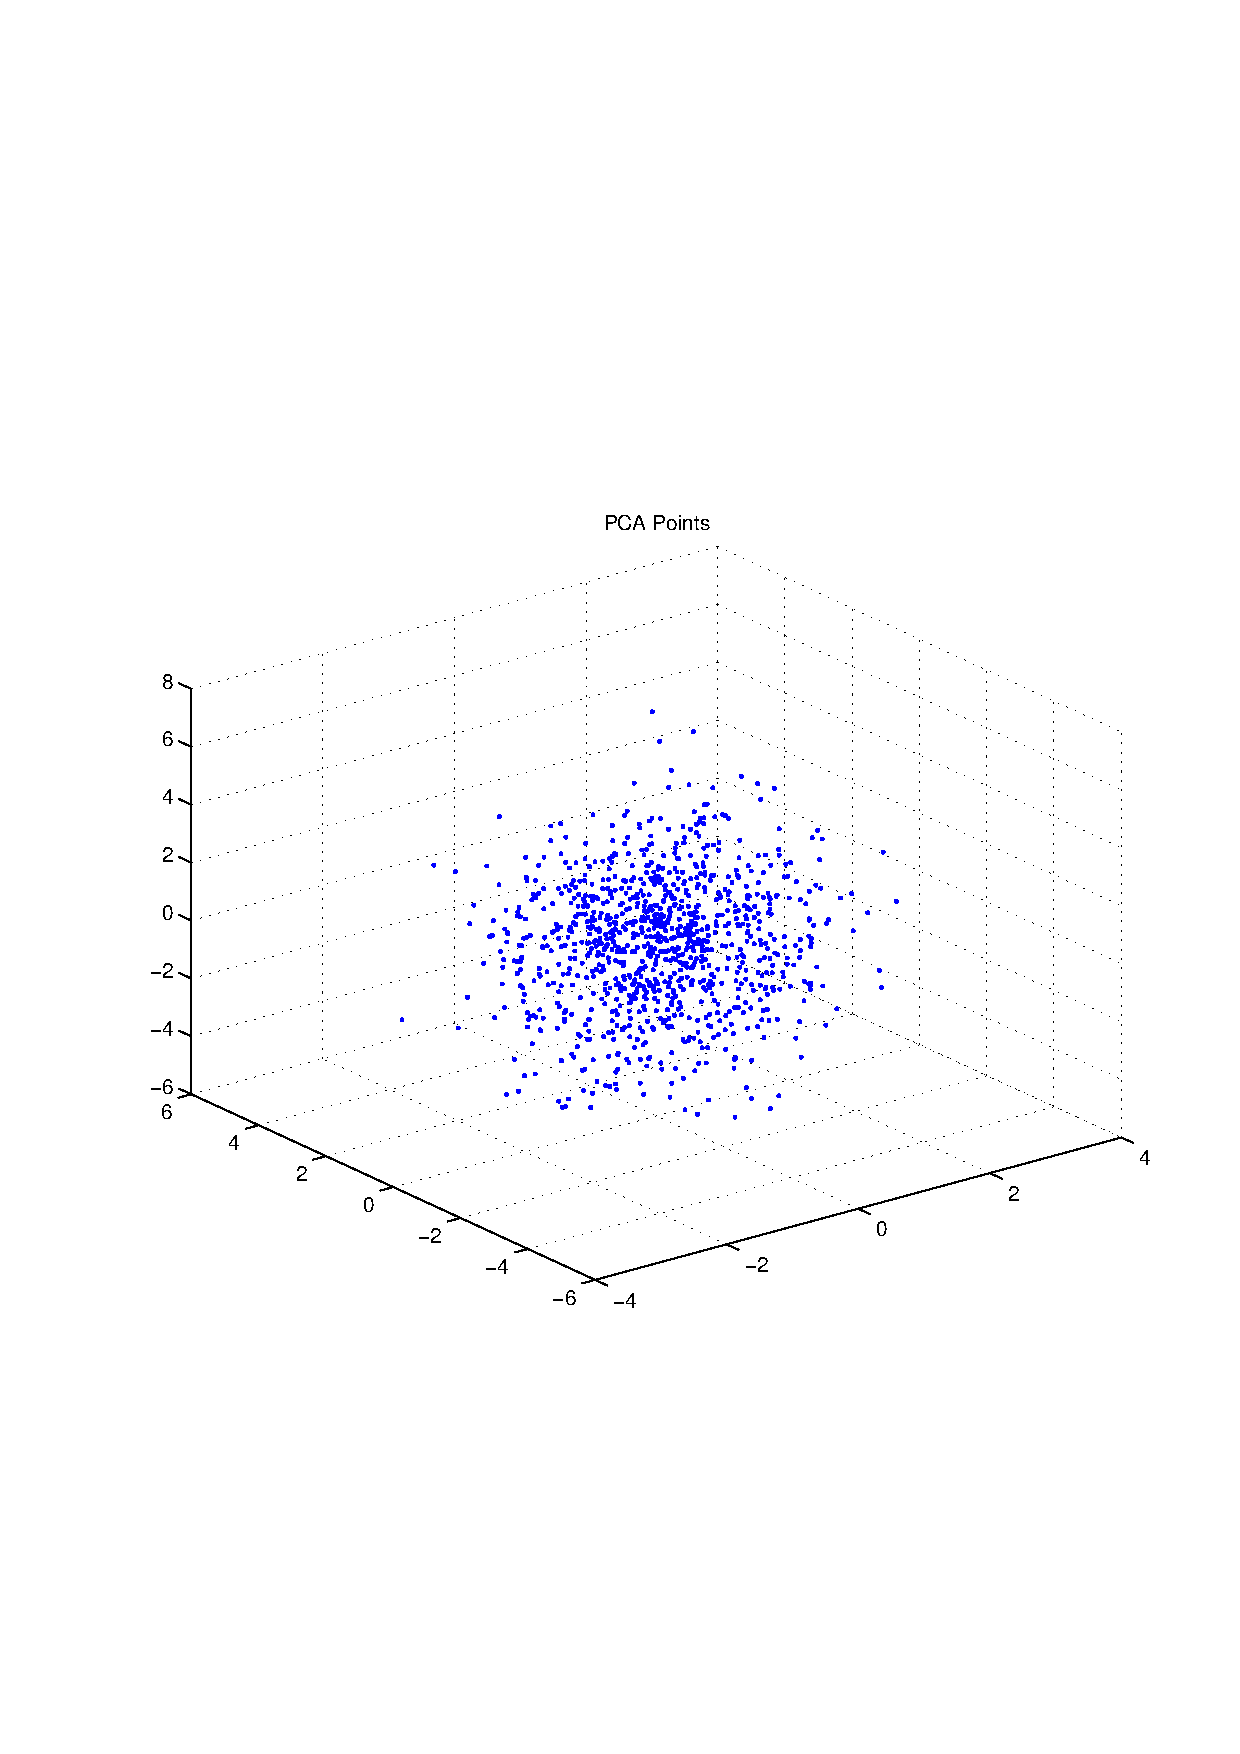
\includegraphics[width=10.0cm,height=10.0cm]{PCAPoints.pdf}

The eigenvectors:
+0.067, +0.331, +0.941
+0.132, +0.932, -0.338
-0.989, +0.147, +0.019

All of the eigenvalues of the covariance matrix:
(+0.958,+0.000), (+2.025,+0.000), (+3.017,+0.000)

QueryPerformanceCounter  =  +0.743
\subsubsection{Multi Variate Random Number Generator }
Sample from $N(\mu,\Sigma)$
mean= -0.002, variance=+1.004, skewness=+0.006, kurtosis=+3.003
mean= -0.001, variance=+1.017, skewness=-0.005, kurtosis=+2.988
mean= -0.002, variance=+1.006, skewness=-0.016, kurtosis=+3.014
Covariance Matrix 
+1.004, +0.009, +0.003
+0.009, +1.017, -0.003
+0.003, -0.003, +1.006

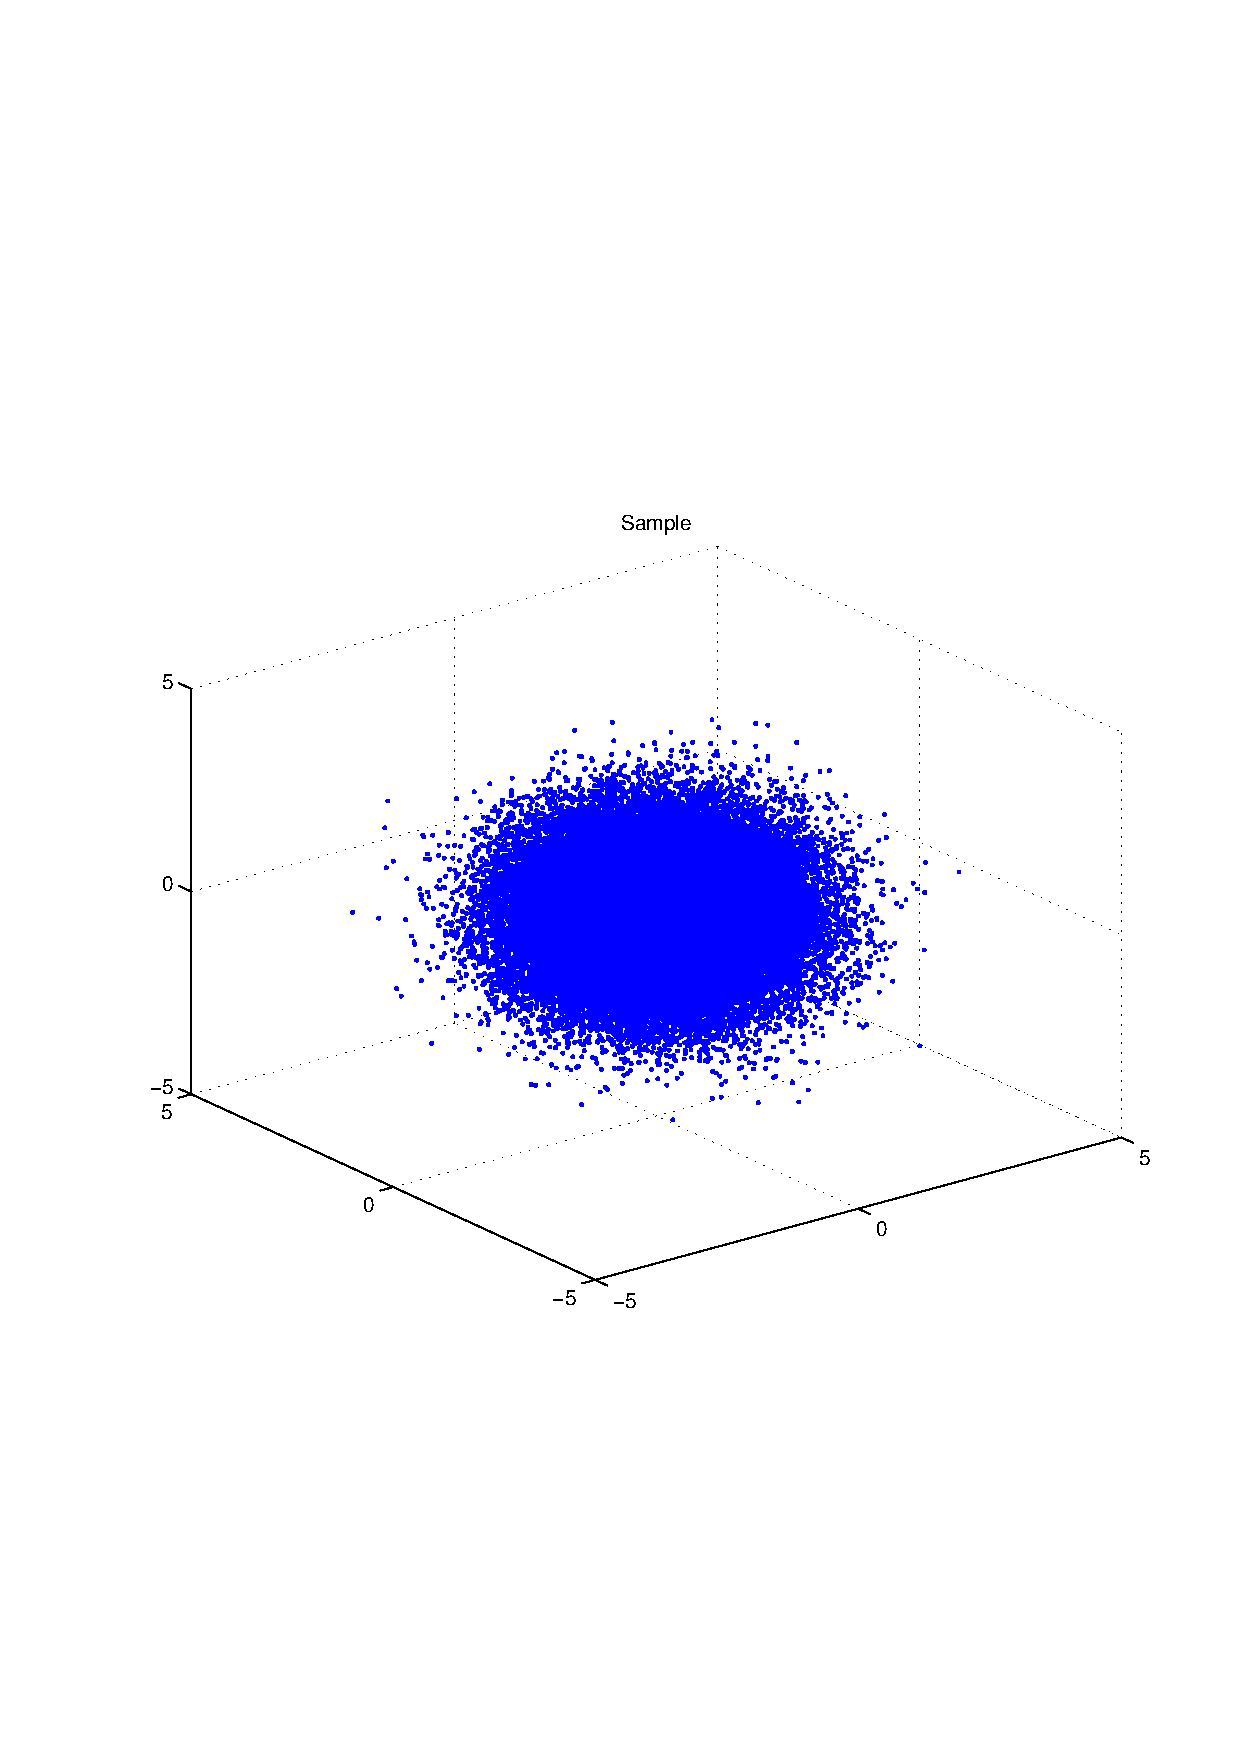
\includegraphics[width=10.0cm,height=10.0cm]{R_3_Normal.pdf}

Generate a sample from a unifom mixture of three Gaussians in $R^3$
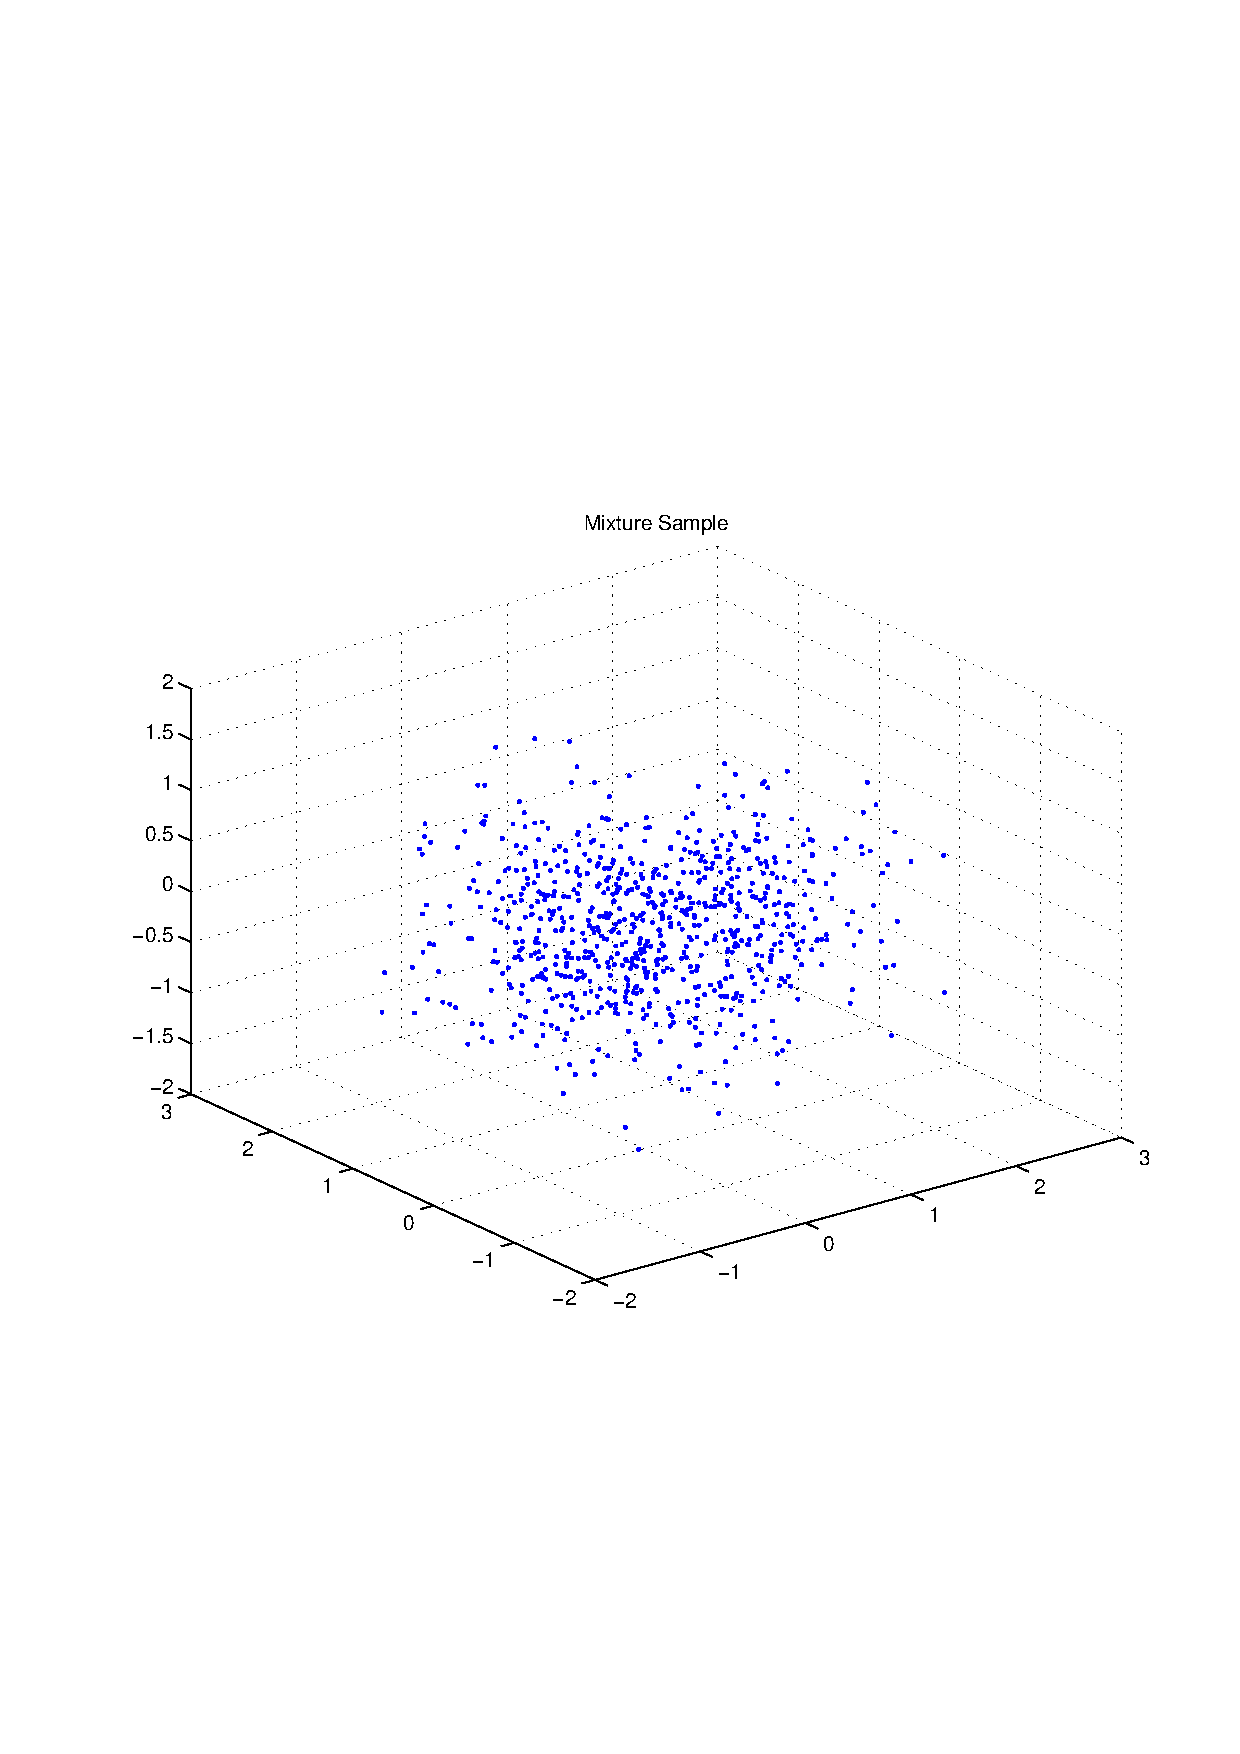
\includegraphics[width=10.0cm,height=10.0cm]{R_3_Normal_Mixture.pdf}

QueryPerformanceCounter  =  +15.113
\subsubsection{Matrix Multiply}
Comparing naive matrix multiply verus Intel MKL dgemm for matrix of size +2048.
This is for type double (hence the d in dgemm).
Naive type double matrix multiply tic toc  =  +2.165
dgemm plus row to column major transpose operation tic toc  =  +1.649
Comparing naive matrix multiply verus Intel MKL sgemm for matrix of size +2048.
This is for type float (hence the s in dgemm).
Naive type float matrix multiply tic toc  =  +1.805
sgemm plus row to column major transpose operation tic toc  =  +1.357
QueryPerformanceCounter  =  +7.835
\subsubsection{Descriptive Statistics}
Mean N(0,1): +0.003
Variance N(0,1): +1.006
Mean N(0,1) [recurrence relation method] :+0.003
Variance [recurrence relation method] :+1.006
Skewness : +0.007
Kurtosis : +2.997
QueryPerformanceCounter  =  +0.034
\subsubsection{Time Series }
+0.093
+0.726
+0.011
+2.178
QueryPerformanceCounter  =  +0.128
\end{document}
